% !TEX program = latexmk
% !TEX encoding = UTF-8 Unicode

\documentclass[11pt,a4paper]{article}

% --- Page / typography ---
\usepackage[a4paper,margin=2.5cm]{geometry}
\usepackage[T1]{fontenc}
\usepackage[utf8]{inputenc}
\usepackage{lmodern}
\usepackage{microtype}

% --- Math ---
\usepackage{amsmath,amssymb,amsthm}
\usepackage{mathtools}

% --- Figures / tables ---
\usepackage{graphicx}
\usepackage{booktabs}
\usepackage{float}
\usepackage{subcaption}

% --- Code listings ---
\usepackage{listings}
\usepackage{xcolor}

\lstset{
  basicstyle=\ttfamily\small,
  backgroundcolor=\color{gray!10},
  frame=single,
  breaklines=true,
  columns=fullflexible,
  keywordstyle=\color{blue},
  commentstyle=\color{gray},
  stringstyle=\color{orange}
}

% --- Links ---
\usepackage[hidelinks]{hyperref}
\usepackage{url}

% --- Graphics path ---
\graphicspath{{img/}}

% --- Algorithm environments ---
\usepackage{algorithm}
\usepackage{algpseudocode}

% --- Theorem environments ---
\theoremstyle{plain}
\newtheorem{theorem}{Theorem}[section]
\newtheorem{lemma}[theorem]{Lemma}

\theoremstyle{definition}
\newtheorem{definition}[theorem]{Definition}

\theoremstyle{remark}
\newtheorem*{remark}{Remark}

% --- Document metadata ---
\title{PCG Arena: A Web Platform for Blind A/B Testing of Procedural Content Generators}
\author{Antoni Czapski}
\date{January 2026}

\begin{document}
\maketitle

\begin{abstract}
Evaluating procedural content generators (PCGs) for video games poses significant methodological challenges, as player enjoyment is inherently subjective and difficult to quantify through automated metrics alone. This report presents \textbf{PCG Arena}, a web-based platform designed for blind A/B testing of Mario level generators through human preference data. The platform enables players to play two procedurally generated levels side-by-side in their browser, vote for their preferred level, and optionally tag gameplay characteristics. Votes are aggregated using the Glicko-2 rating system, which provides uncertainty-aware rankings with confidence intervals.

Key technical contributions include: (1) a browser-based Mario game engine faithfully ported from Java to TypeScript, (2) an adaptive matchmaking algorithm (AGIS) that optimizes for rapid rating convergence, (3) a builder profile system enabling researchers to submit and compete with their own generators, and (4) comprehensive research analytics including death heatmaps, player trajectories, and confusion matrices.

The platform is deployed at \url{https://pcg-arena.com}, featuring Google OAuth and email/password authentication, Twilio SendGrid integration for email verification, and Docker-based deployment on Google Cloud Platform. This work provides the research community with an accessible tool for empirically comparing procedural content generators through human evaluation.
\end{abstract}

\tableofcontents
\newpage

%==============================================================================
\section{Introduction}
\label{sec:introduction}
%==============================================================================

Procedural Content Generation (PCG) has become a cornerstone of modern game development, enabling the automatic creation of game levels, narratives, textures, and other assets~\cite{summerville2018}. However, evaluating the quality of procedurally generated content remains a fundamental challenge in the field. While automated metrics such as playability, diversity, and structural features provide valuable insights, they often fail to capture the subjective experience of human players---the ultimate consumers of generated content.

The Mario AI Championship's Level Generation Track~\cite{marioai} established a precedent for human evaluation of PCG by having players experience and compare levels from different generators. However, such competitions typically rely on controlled laboratory settings with limited participants, making it difficult to gather statistically significant preference data at scale.

This project addresses these limitations by developing \textbf{PCG Arena}, a fully operational web platform that enables:

\begin{enumerate}
    \item \textbf{Browser-Based Gameplay}: Players can experience Mario levels directly in their browser without downloading any software, removing the primary barrier to participation.
    
    \item \textbf{Blind A/B Testing}: Each battle presents two levels from different generators without revealing their source, eliminating bias from generator reputation.
    
    \item \textbf{Uncertainty-Aware Rankings}: The Glicko-2 rating system provides not only point estimates of generator quality but also confidence intervals that reflect the reliability of those estimates.
    
    \item \textbf{Adaptive Matchmaking}: The AGIS (Adaptive Glicko-Informed Selection) algorithm prioritizes matchups that maximize information gain, ensuring efficient convergence of ratings.
    
    \item \textbf{Research Analytics}: Comprehensive data collection enables analysis of player preferences, level difficulty, and engagement patterns.
\end{enumerate}

The platform is live at \url{https://pcg-arena.com} and serves as both a practical tool for PCG researchers and a demonstration of modern web technologies for game-based research.

This report is structured as follows: Section~\ref{sec:background} provides background on PCG and rating systems. Section~\ref{sec:architecture} describes the system architecture. Sections~\ref{sec:engine}--\ref{sec:admin} detail the core components. Section~\ref{sec:deployment} covers infrastructure, and Section~\ref{sec:results} presents preliminary results.

%==============================================================================
\section{Background and Related Work}
\label{sec:background}
%==============================================================================

\subsection{Procedural Content Generation}
\label{subsec:pcg}

Procedural Content Generation refers to the algorithmic creation of game content with limited or indirect human input~\cite{summerville2018}. PCG techniques range from simple rule-based systems to sophisticated machine learning approaches, including:

\begin{itemize}
    \item \textbf{Search-Based PCG}: Using evolutionary algorithms to optimize levels against fitness functions measuring playability, difficulty, and aesthetics.
    \item \textbf{Grammar-Based PCG}: Defining formal grammars that specify valid level structures and generating content through grammar expansion.
    \item \textbf{Machine Learning PCG (PCGML)}: Training neural networks on existing human-designed content to learn implicit design patterns~\cite{summerville2018}.
\end{itemize}

A fundamental challenge in PCG research is evaluation: how do we determine whether one generator produces ``better'' content than another? This question motivates the development of PCG Arena.

\subsection{Mario AI Framework}
\label{subsec:mario-ai}

The Mario AI Framework~\cite{marioai} provides a standardized environment for AI research in platformer games. Originally developed for the Mario AI Competition, it offers:

\begin{itemize}
    \item A faithful recreation of Super Mario Bros. physics and mechanics
    \item A standardized ASCII level format for representing tile-based levels
    \item APIs for both playing agents and level generators
    \item Tools for level analysis and visualization
\end{itemize}

PCG Arena builds upon this framework, using its level format and adapting its physics engine for browser-based gameplay. The ASCII tilemap format represents levels as grids of characters, where each character denotes a specific tile type (ground, brick, enemy spawn, etc.).

\subsection{Human Evaluation in PCG}
\label{subsec:human-eval}

Human evaluation remains the gold standard for assessing game content quality~\cite{marioai}. Common approaches include:

\begin{itemize}
    \item \textbf{Absolute Rating}: Players rate individual levels on a numerical scale (e.g., 1--5 stars).
    \item \textbf{Pairwise Comparison}: Players compare two items and choose their preference.
    \item \textbf{Ranking}: Players order multiple items from best to worst.
\end{itemize}

Pairwise comparison, the method used by PCG Arena, offers several advantages: it reduces cognitive load compared to absolute rating, produces more consistent results across participants, and maps naturally to ranking algorithms like Elo and Glicko-2.

\subsection{Rating Systems for Pairwise Comparisons}
\label{subsec:rating-systems}

Rating systems for pairwise comparisons originated in chess and have been widely adopted for competitive games and recommendation systems. The Elo rating system, developed by Arpad Elo, models the probability of player A defeating player B based on their rating difference:

\begin{equation}
P(A \text{ wins}) = \frac{1}{1 + 10^{(R_B - R_A)/400}}
\end{equation}

The Glicko-2 system~\cite{glickman2012} extends Elo by adding two additional parameters:

\begin{itemize}
    \item \textbf{Rating Deviation (RD)}: Measures uncertainty in the rating estimate. New or inactive players have high RD; active players converge to low RD.
    \item \textbf{Volatility ($\sigma$)}: Captures the expected fluctuation in performance over time.
\end{itemize}

PCG Arena uses Glicko-2 because its uncertainty quantification directly addresses a key research need: knowing not just which generator is best, but how confident we can be in that ranking.

%==============================================================================
\section{System Architecture}
\label{sec:architecture}
%==============================================================================

\subsection{High-Level Overview}
\label{subsec:arch-overview}

PCG Arena follows a classic three-tier web architecture with clear separation of concerns:

\begin{enumerate}
    \item \textbf{Presentation Layer}: React/TypeScript frontend running in the user's browser
    \item \textbf{Application Layer}: Python/FastAPI backend handling business logic and API endpoints
    \item \textbf{Data Layer}: SQLite database persisting all platform state
\end{enumerate}

Figure~\ref{fig:architecture} illustrates the high-level system architecture. Users interact with the platform through a browser-based frontend that communicates with the backend via a RESTful API following the \texttt{arena/v0} protocol specification.

\begin{figure}[H]
    \centering
    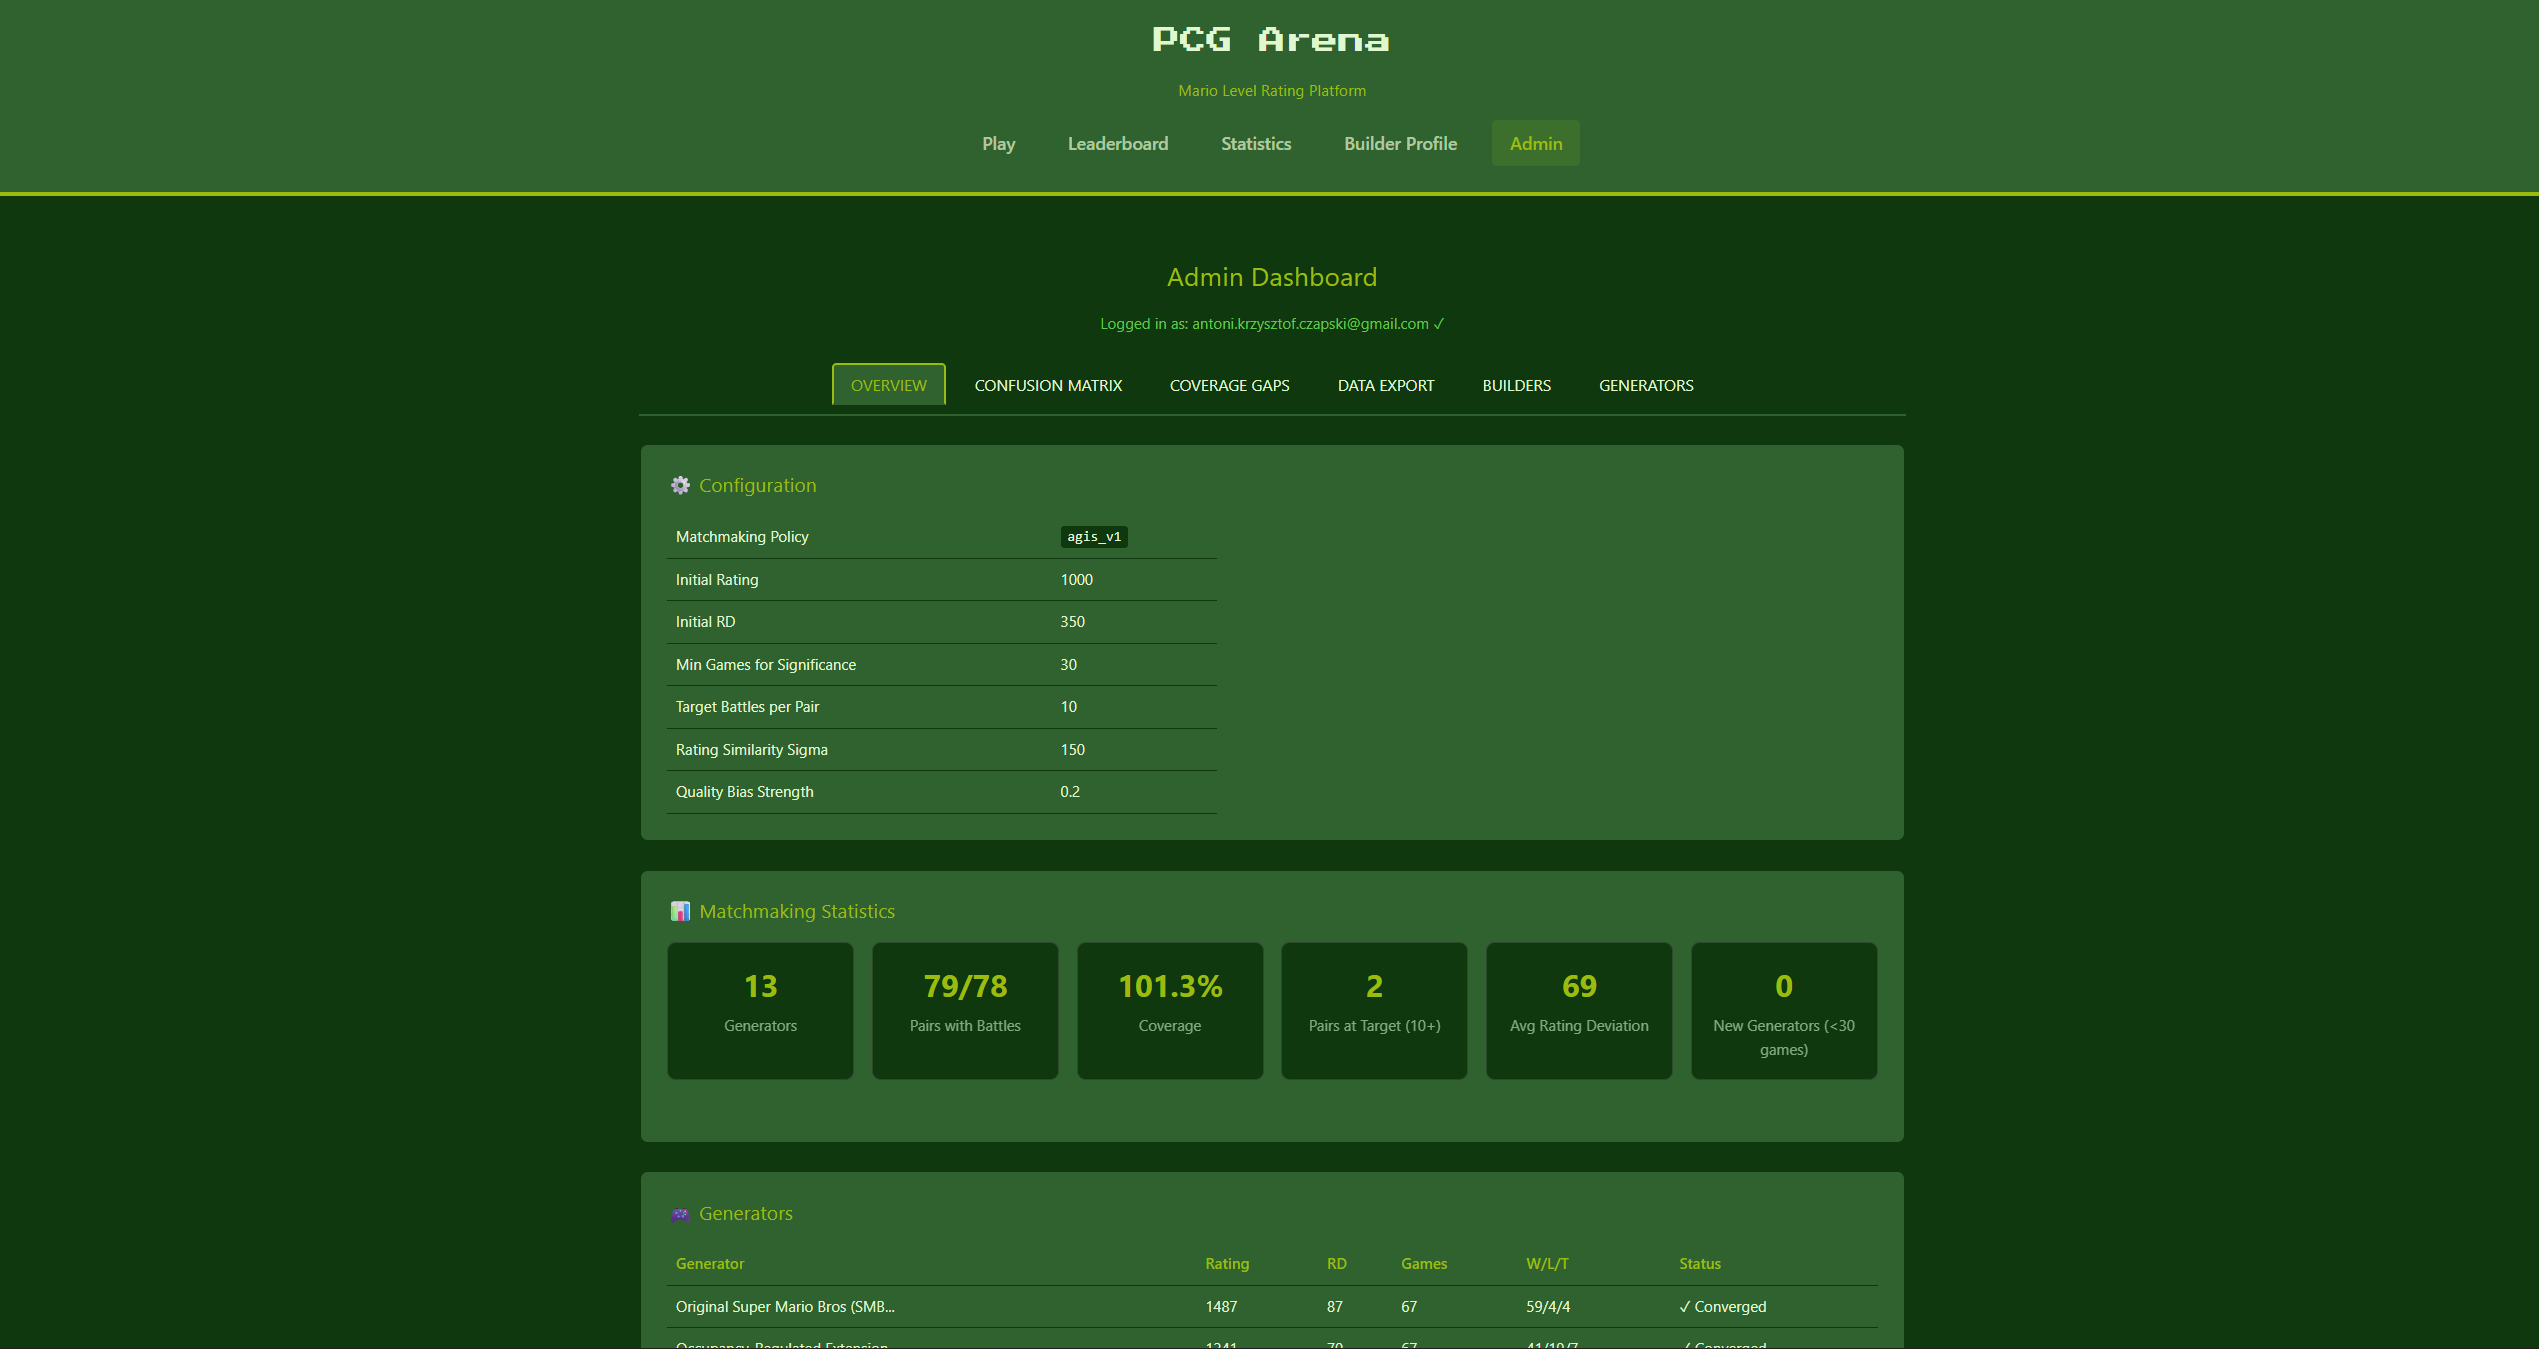
\includegraphics[width=0.9\textwidth]{admin_overview.png}
    \caption{Admin overview showing system architecture and platform statistics.}
    \label{fig:architecture}
\end{figure}

\subsection{Backend Architecture}
\label{subsec:backend}

The backend is implemented in Python using the FastAPI framework, chosen for its:

\begin{itemize}
    \item Automatic OpenAPI documentation generation
    \item Native async/await support for concurrent request handling
    \item Built-in request validation via Pydantic models
    \item High performance comparable to Node.js and Go
\end{itemize}

Key backend modules include:

\begin{itemize}
    \item \texttt{main.py}: FastAPI application with route definitions
    \item \texttt{auth.py}: Authentication logic (Google OAuth, email/password)
    \item \texttt{glicko2.py}: Glicko-2 rating system implementation
    \item \texttt{matchmaking.py}: AGIS matchmaking algorithm
    \item \texttt{builders.py}: Generator submission and management
    \item \texttt{stats.py}: Research analytics and data export
\end{itemize}

The backend runs in a Docker container, ensuring consistent deployment across environments.

\subsection{Frontend Architecture}
\label{subsec:frontend}

The frontend is built with React 18 and TypeScript 5.6, using Vite as the build tool. Key architectural decisions include:

\begin{itemize}
    \item \textbf{Component-Based Design}: UI elements are reusable React components
    \item \textbf{Canvas-Based Rendering}: Game graphics use HTML5 Canvas for direct pixel manipulation
    \item \textbf{Type Safety}: TypeScript catches errors at compile time
    \item \textbf{Fast Development}: Vite provides sub-second hot module replacement
\end{itemize}

The frontend directory structure separates concerns:

\begin{lstlisting}
frontend/src/
  api/           # Backend communication
  engine/        # Game engine (ported from Java)
  components/    # React UI components
  pages/         # Full page components
  contexts/      # React state management
\end{lstlisting}

\subsection{Database Design}
\label{subsec:database}

PCG Arena uses SQLite for data persistence, chosen for:

\begin{itemize}
    \item Single-file storage simplifying backups and deployment
    \item ACID transactions ensuring data consistency
    \item Zero configuration and no separate database service
    \item Sufficient performance for the expected load
\end{itemize}

The database schema comprises 17 tables across 17 migrations:

\begin{table}[H]
\centering
\begin{tabular}{ll}
\toprule
\textbf{Table} & \textbf{Purpose} \\
\midrule
\texttt{generators} & PCG algorithm metadata with owner reference \\
\texttt{levels} & ASCII tilemap levels with content hash \\
\texttt{battles} & Comparison instances pairing two levels \\
\texttt{votes} & User outcomes with telemetry data \\
\texttt{ratings} & Glicko-2 ratings per generator \\
\texttt{rating\_events} & Audit log of rating changes \\
\texttt{users} & Authenticated user accounts \\
\texttt{user\_sessions} & Active login sessions \\
\texttt{play\_trajectories} & Player position and death data \\
\bottomrule
\end{tabular}
\caption{Key database tables in PCG Arena.}
\label{tab:db-tables}
\end{table}

%==============================================================================
\section{Game Engine Implementation}
\label{sec:engine}
%==============================================================================

\subsection{TypeScript Port from Java}
\label{subsec:ts-port}

A critical component of PCG Arena is the browser-based Mario game engine, which was ported from the Java-based Mario AI Framework to TypeScript. This port required careful attention to maintain gameplay fidelity while adapting to browser constraints.

The porting process involved:

\begin{enumerate}
    \item \textbf{Class Structure Translation}: Java classes were converted to TypeScript classes, preserving inheritance hierarchies and encapsulation.
    \item \textbf{Physics Constants Preservation}: All physics constants were kept identical to ensure matching gameplay feel.
    \item \textbf{Rendering System Adaptation}: Java's Swing/AWT rendering was replaced with HTML5 Canvas.
    \item \textbf{Input System Rewrite}: Keyboard input handling was reimplemented for browser events.
\end{enumerate}

Key engine modules include:

\begin{lstlisting}
engine/
  MarioGame.ts       # Game loop (requestAnimationFrame)
  MarioWorld.ts      # World state and game logic
  MarioLevel.ts      # Level parsing from ASCII
  MarioSprite.ts     # Base sprite class
  sprites/           # Mario, enemies, items
  graphics/          # Camera, rendering
  effects/           # Visual effects (particles)
\end{lstlisting}

\subsection{Physics and Gameplay}
\label{subsec:physics}

The game engine preserves exact physics constants from the Java version to ensure identical gameplay:

\begin{table}[H]
\centering
\begin{tabular}{lr}
\toprule
\textbf{Parameter} & \textbf{Value} \\
\midrule
Ground Inertia & 0.89 \\
Air Inertia & 0.89 \\
Gravity & 3.0 \\
Jump Velocity & $-1.9$ \\
Walk Speed & 0.6 \\
Run Speed & 1.2 \\
\bottomrule
\end{tabular}
\caption{Core physics constants in the Mario engine.}
\label{tab:physics}
\end{table}

The game loop runs at 30 ticks per second (matching the original), with rendering at 60 FPS using \texttt{requestAnimationFrame}. Physics updates are deterministic, ensuring consistent gameplay across sessions.

\subsection{Level Format and Parsing}
\label{subsec:level-format}

Levels are represented as ASCII tilemaps, where each character corresponds to a tile type:

\begin{lstlisting}
--------------          (empty space)
----------S---          (S = breakable brick)
---E---Q------          (E = enemy, Q = question block)
##############          (# = ground)
\end{lstlisting}

The level parser (\texttt{MarioLevel.ts}) processes these tilemaps, converting characters to internal tile representations and spawning sprite entities for enemies and items. Validation rules ensure levels are playable:

\begin{itemize}
    \item Minimum dimensions: $50 \times 16$ tiles
    \item Maximum dimensions: $500 \times 16$ tiles
    \item Required: Mario spawn point and exit flag
    \item Prohibited: Unreachable exits, instant-death spawns
\end{itemize}

%==============================================================================
\section{Battle and Voting System}
\label{sec:voting}
%==============================================================================

\subsection{Battle Flow}
\label{subsec:battle-flow}

The core user experience of PCG Arena is the ``battle''---a blind A/B test where players compare two levels from different generators. The battle flow proceeds as follows:

\begin{enumerate}
    \item \textbf{Battle Request}: The frontend requests a new battle from \texttt{POST /v1/battles:next}.
    \item \textbf{Matchmaking}: The AGIS algorithm selects two generators and one random level from each.
    \item \textbf{Gameplay}: The player plays both levels sequentially (left then right).
    \item \textbf{Voting}: After playing both, the player votes for their preference.
    \item \textbf{Rating Update}: The backend updates Glicko-2 ratings atomically.
\end{enumerate}

Figure~\ref{fig:gameplay} shows the main gameplay interface where players experience levels side-by-side.

\begin{figure}[H]
    \centering
    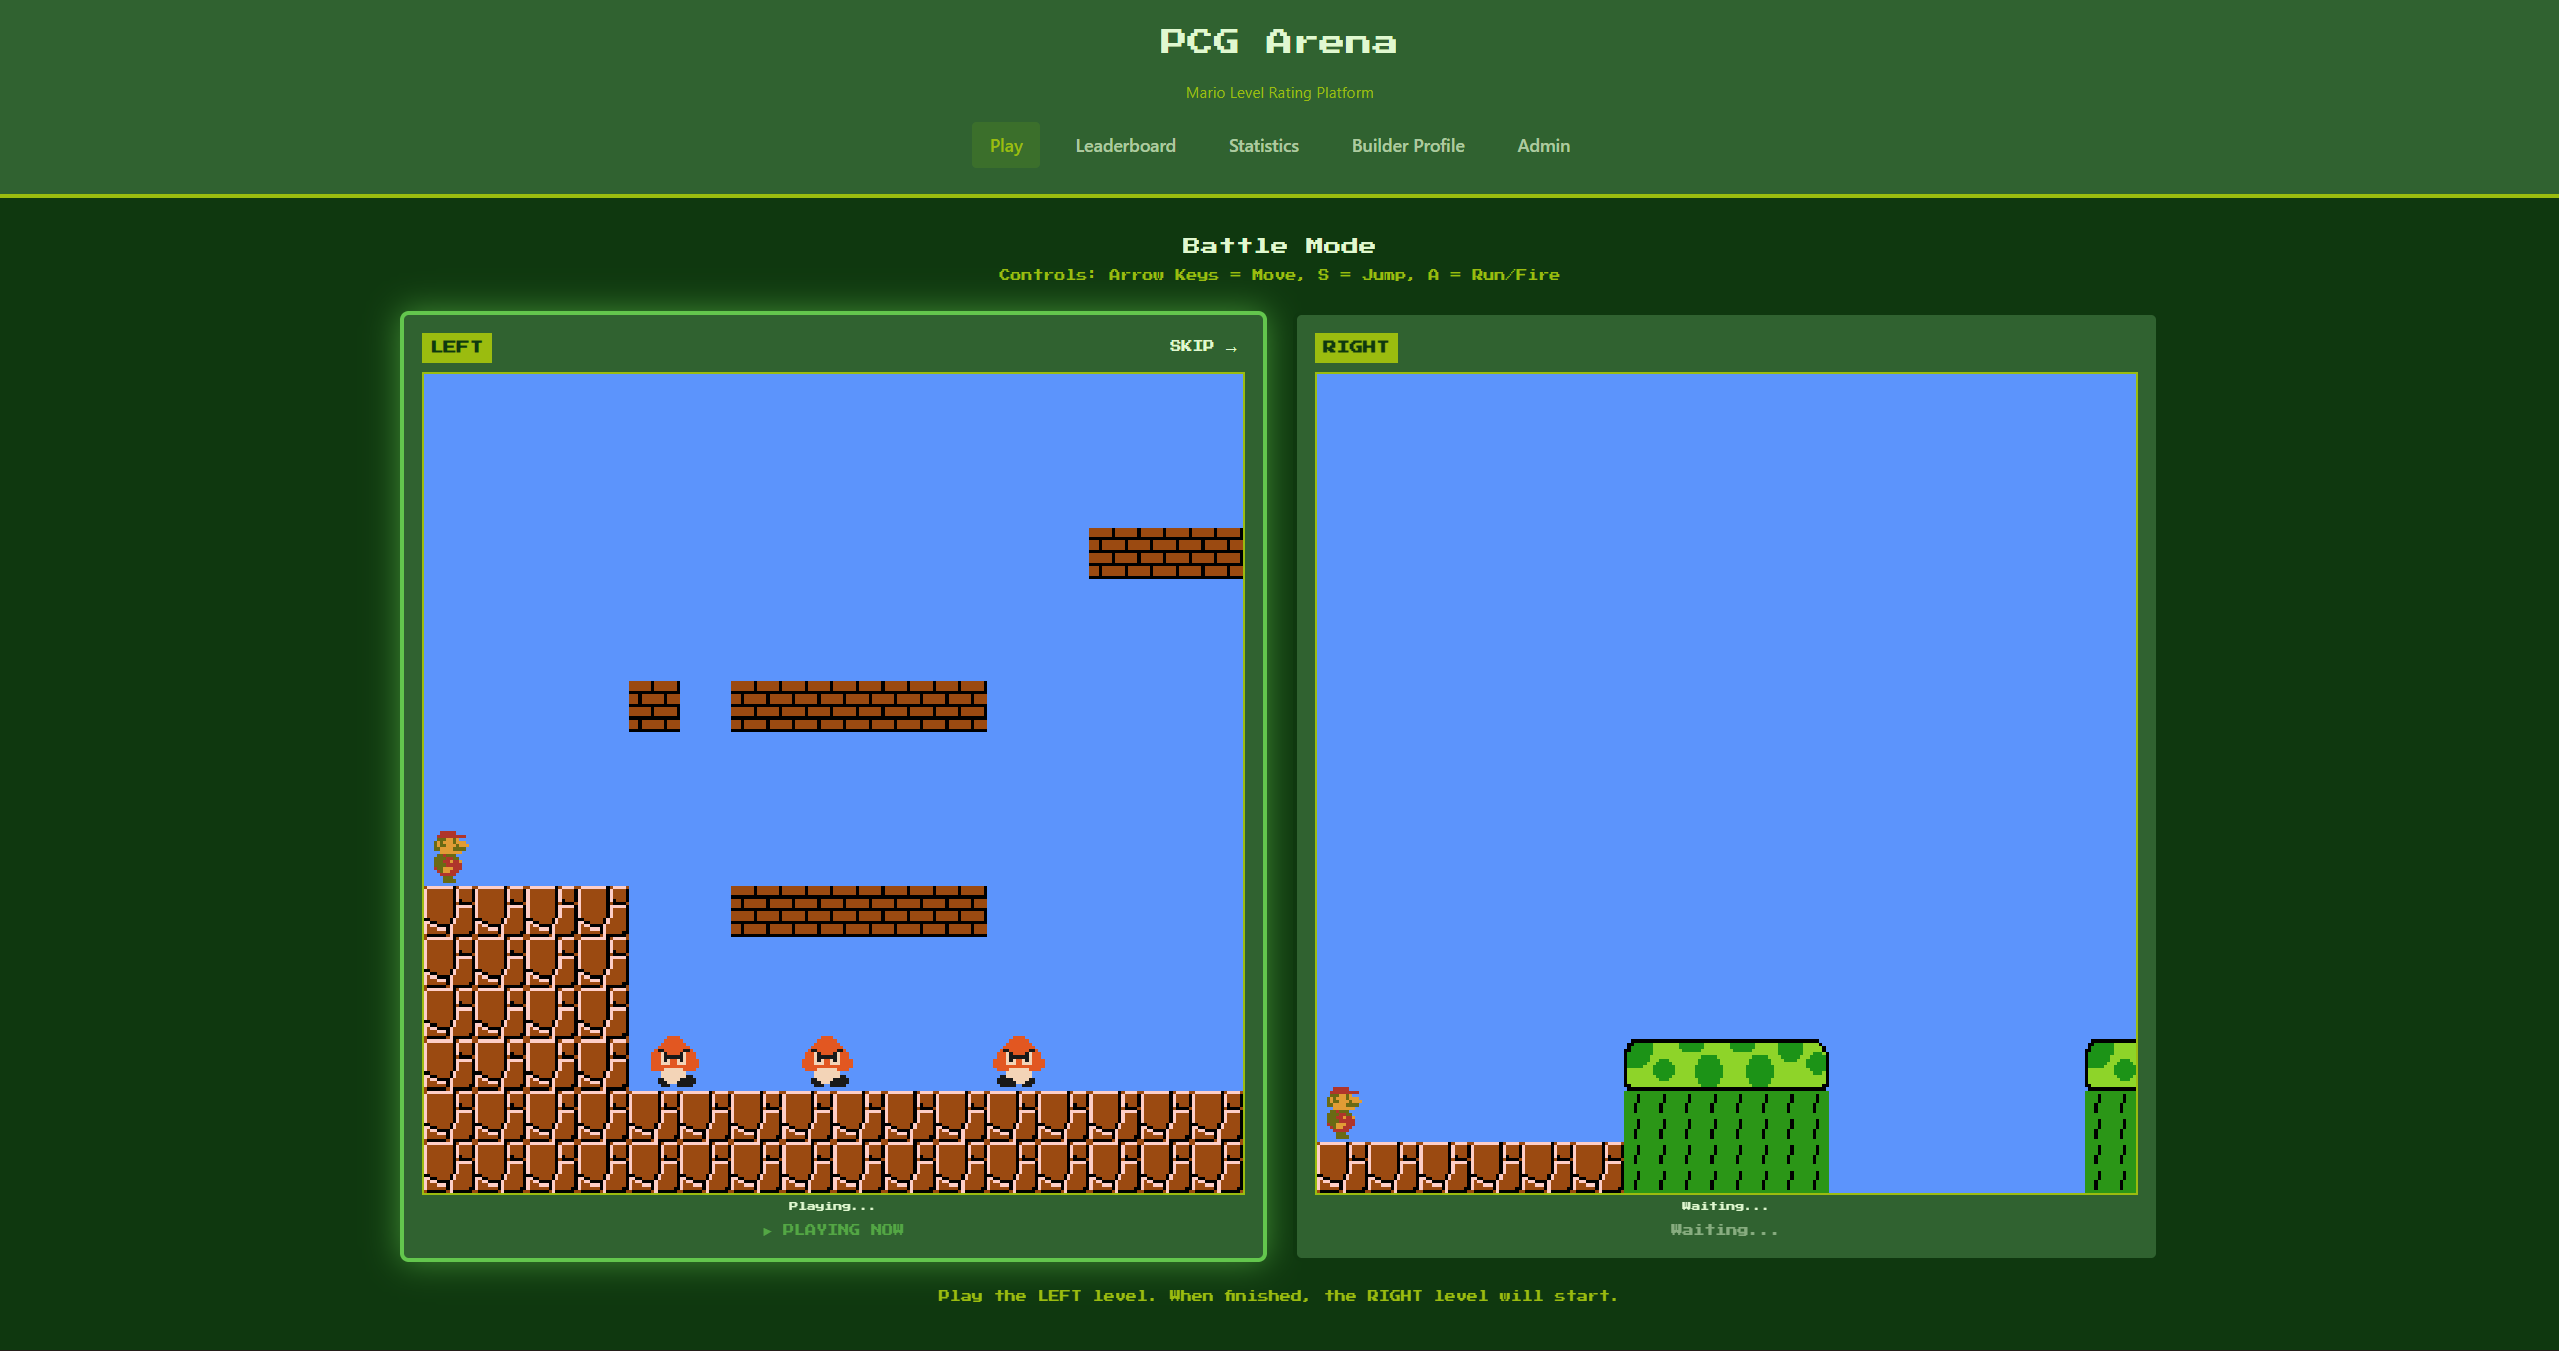
\includegraphics[width=0.95\textwidth]{main_gameplay.png}
    \caption{Main gameplay view showing the active level with game controls and timer.}
    \label{fig:gameplay}
\end{figure}

\subsection{Voting Interface}
\label{subsec:voting-interface}

After completing both levels, players are presented with the voting interface (Figure~\ref{fig:voting}). The interface displays:

\begin{itemize}
    \item Static visualizations of both complete levels for reference
    \item Vote buttons: ``Left is Better,'' ``Right is Better,'' ``Tie,'' ``Skip''
    \item Optional tagging interface for additional feedback
\end{itemize}

\begin{figure}[H]
    \centering
    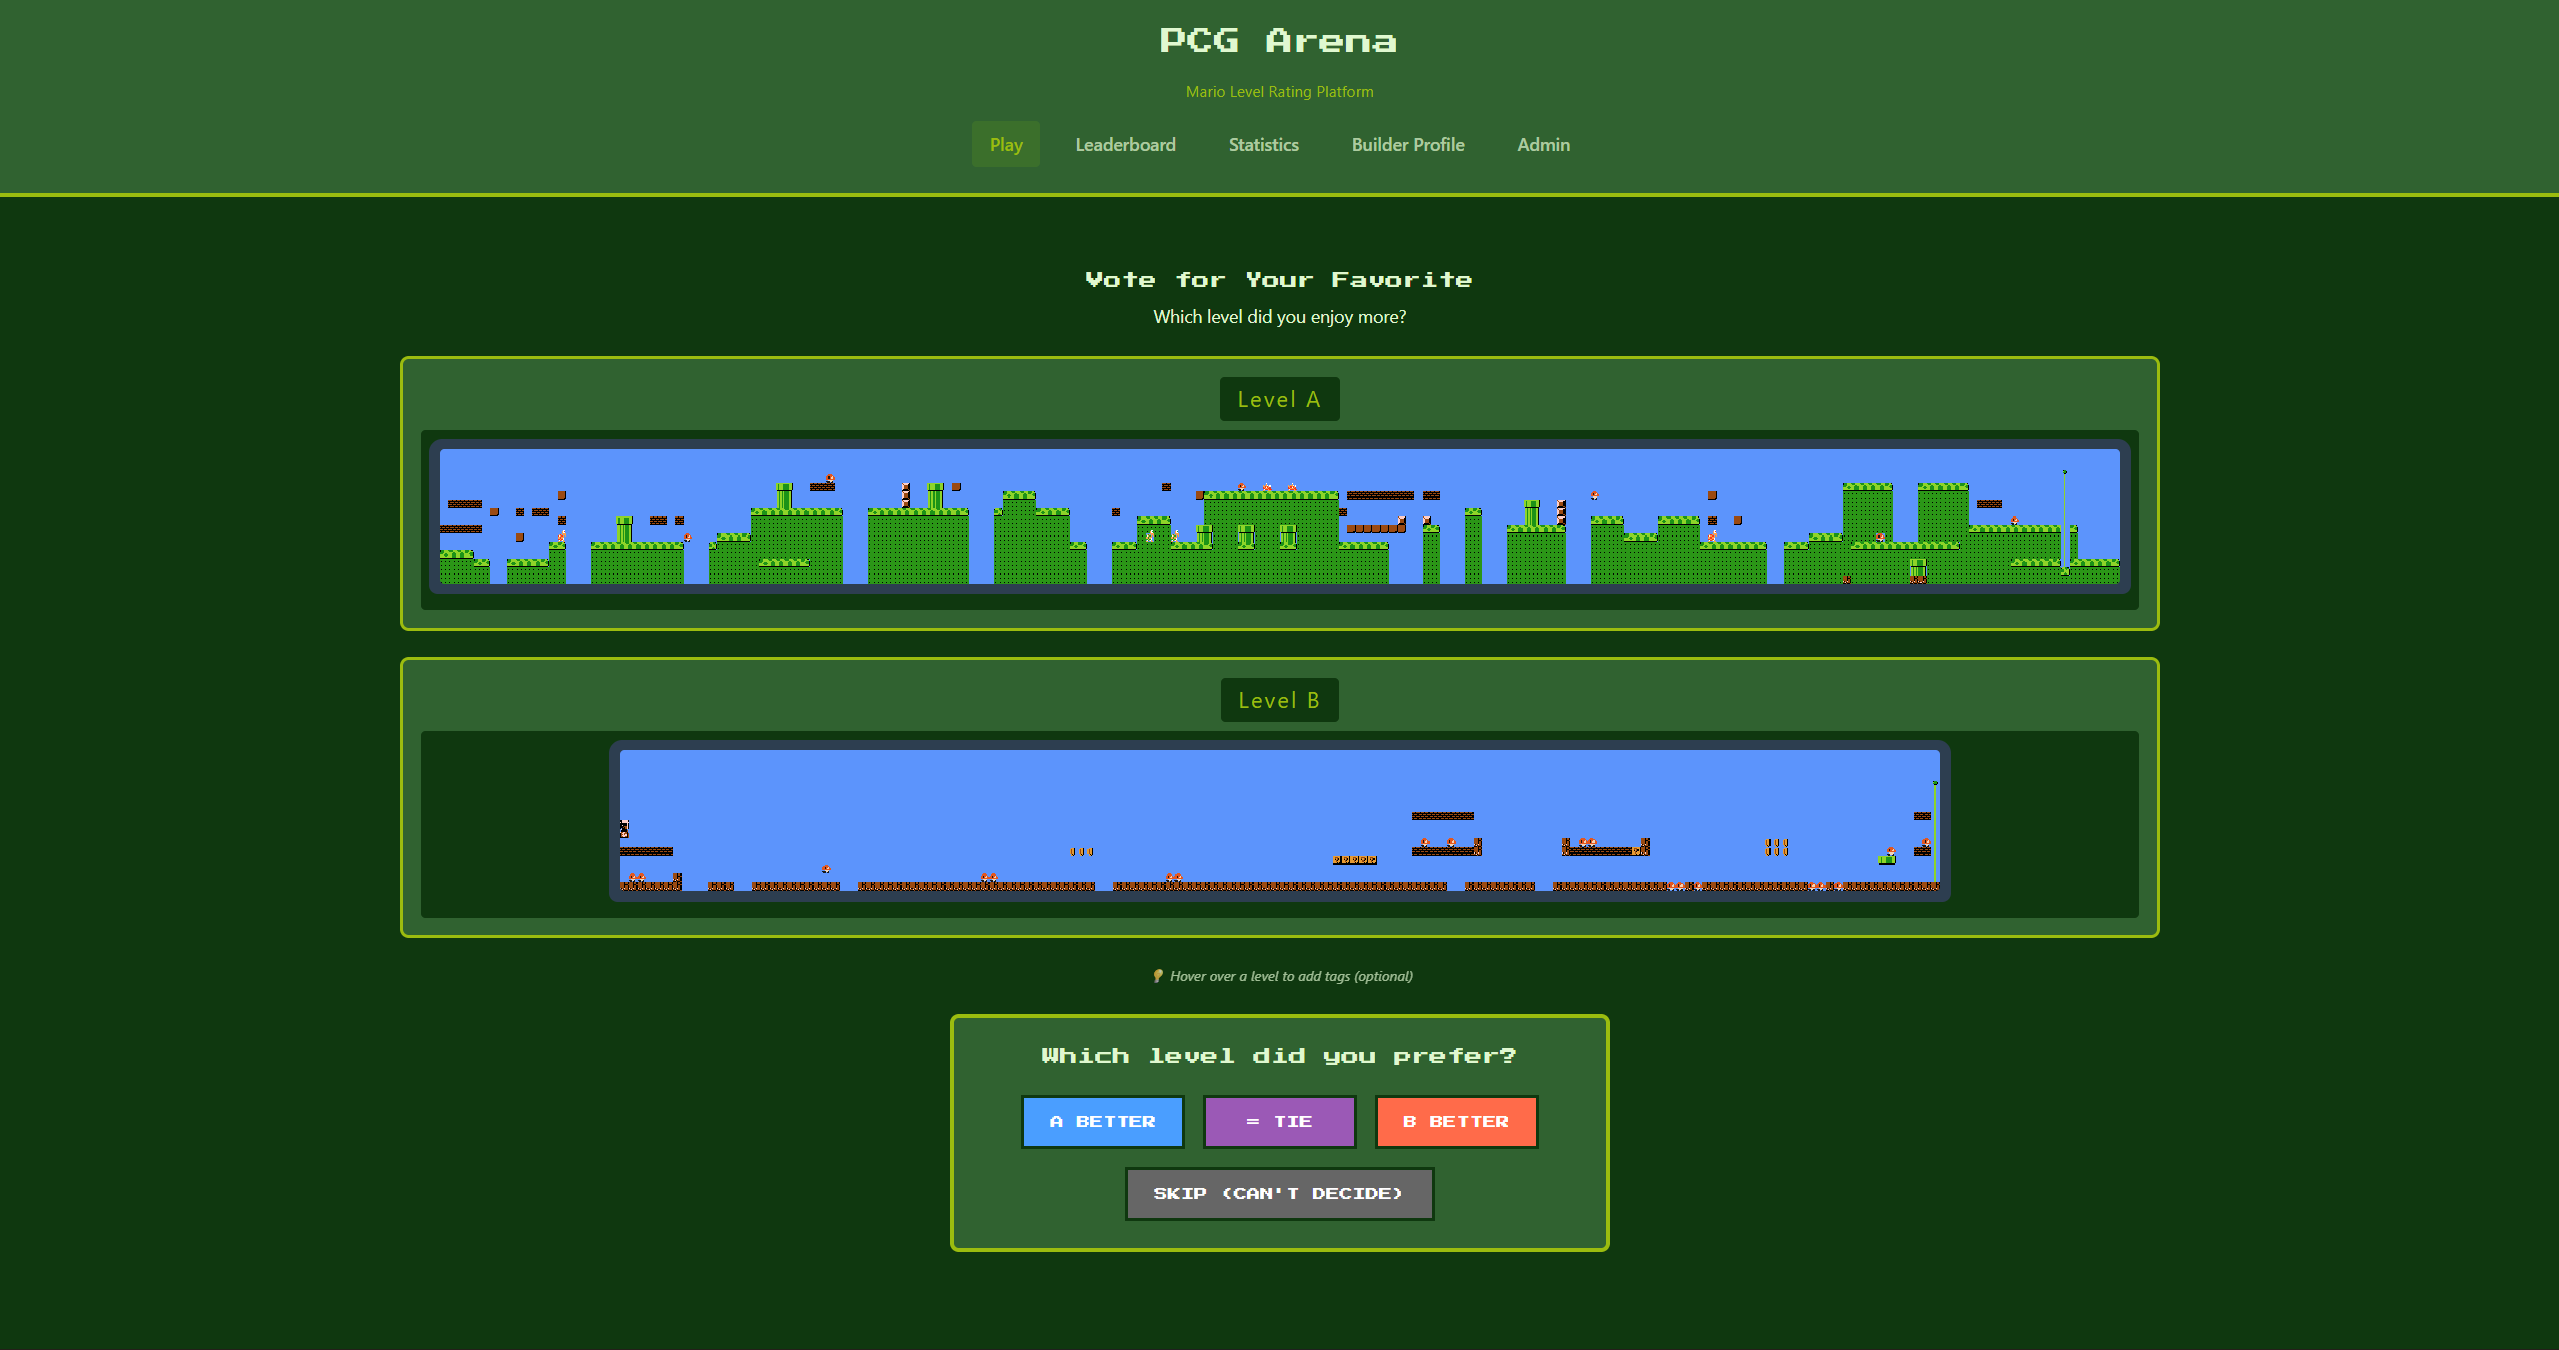
\includegraphics[width=0.9\textwidth]{voting_panel.png}
    \caption{Voting panel showing level previews and vote options after gameplay.}
    \label{fig:voting}
\end{figure}

The ``Skip'' option allows players to abstain from voting if they encountered technical issues or feel unable to judge. Skipped battles do not affect ratings.

\subsection{Tagging System}
\label{subsec:tagging}

In addition to the binary preference vote, players can optionally tag each level with descriptive labels. Tags capture qualitative aspects that the vote alone cannot express:

\begin{table}[H]
\centering
\begin{tabular}{ll}
\toprule
\textbf{Category} & \textbf{Tags} \\
\midrule
Difficulty & too-easy, just-right, too-hard \\
Design & creative, boring, frustrating, fun \\
Structure & linear, exploration, puzzle-like \\
Issues & broken, impossible, unplayable \\
\bottomrule
\end{tabular}
\caption{Available tags for level characterization.}
\label{tab:tags}
\end{table}

Tag data enables richer analysis, such as correlating perceived difficulty with win rates or identifying generators that produce consistently ``frustrating'' levels.

%==============================================================================
\section{Matchmaking Algorithm}
\label{sec:matchmaking}
%==============================================================================

\subsection{Problem Definition}
\label{subsec:matchmaking-problem}

The matchmaking problem in PCG Arena is: given $n$ generators with current ratings and uncertainties, select a pair for the next battle that maximizes information gain toward accurate final rankings.

Naive approaches fail:

\begin{itemize}
    \item \textbf{Uniform Random}: Wastes battles on already-converged pairs.
    \item \textbf{Most Uncertain First}: May neglect head-to-head comparisons between similar generators.
    \item \textbf{Round-Robin}: Ignores rating information; pairs dissimilar generators.
\end{itemize}

The ideal matchmaking algorithm should:

\begin{enumerate}
    \item Prioritize generators with high uncertainty (new or rarely played)
    \item Prefer matchups between generators of similar skill levels
    \item Ensure all pairs get sufficient battles for the confusion matrix
    \item Converge quickly to stable rankings
\end{enumerate}

\subsection{AGIS: Adaptive Glicko-Informed Selection}
\label{subsec:agis}

We developed \textbf{AGIS (Adaptive Glicko-Informed Selection)}, a matchmaking algorithm that uses Glicko-2 rating information to optimize battle selection. AGIS operates in two stages:

\textbf{Stage 1: First Generator Selection}

Each generator $i$ receives a selection weight $w_i$ based on:

\begin{equation}
w_i = (1 + \text{RD}_{\text{norm}, i})^2 \cdot \text{boost}(\text{games}_i) \cdot (1 + \alpha \cdot \text{quality}_i)
\end{equation}

where $\text{RD}_{\text{norm}}$ is the normalized rating deviation (high = uncertain), $\text{boost}$ amplifies weight for generators with few games, and $\text{quality}$ provides slight bias toward higher-rated generators after convergence.

\textbf{Stage 2: Second Generator Selection}

Given the first generator $g_1$, the second generator is selected with weight:

\begin{equation}
w_{1,j} = \alpha \cdot S(g_1, g_j) + \beta \cdot U(g_j) + \gamma \cdot C(g_1, g_j)
\end{equation}

where:
\begin{itemize}
    \item $S(g_1, g_j)$: Rating similarity (Gaussian decay from rating difference)
    \item $U(g_j)$: Uncertainty factor (based on $g_j$'s RD)
    \item $C(g_1, g_j)$: Coverage factor (inverse of pair's battle count)
\end{itemize}

\subsection{Generator Selection Weights}
\label{subsec:selection-weights}

The configurable parameters of AGIS (with defaults) are:

\begin{table}[H]
\centering
\begin{tabular}{llr}
\toprule
\textbf{Parameter} & \textbf{Description} & \textbf{Default} \\
\midrule
\texttt{AGIS\_MIN\_GAMES} & Games before ``converged'' & 30 \\
\texttt{AGIS\_TARGET\_BATTLES\_PER\_PAIR} & Minimum battles per pair & 10 \\
\texttt{AGIS\_RATING\_SIGMA} & Rating similarity std dev & 150.0 \\
\texttt{AGIS\_QUALITY\_BIAS} & Quality bias strength & 0.2 \\
\midrule
$\alpha$ & Rating similarity weight & 0.5 \\
$\beta$ & Uncertainty weight & 0.3 \\
$\gamma$ & Coverage weight & 0.2 \\
\bottomrule
\end{tabular}
\caption{AGIS algorithm parameters.}
\label{tab:agis-params}
\end{table}

%==============================================================================
\section{Rating System}
\label{sec:rating}
%==============================================================================

\subsection{Glicko-2 Algorithm}
\label{subsec:glicko2}

PCG Arena uses the Glicko-2 rating system~\cite{glickman2012}, which maintains three parameters for each generator:

\begin{itemize}
    \item \textbf{Rating ($\mu$)}: The skill estimate, displayed on a scale centered at 1000.
    \item \textbf{Rating Deviation (RD, $\phi$)}: The uncertainty in the rating. High RD means unreliable rating.
    \item \textbf{Volatility ($\sigma$)}: Expected fluctuation in performance over time.
\end{itemize}

The expected score when generator $A$ plays against generator $B$ is:

\begin{equation}
E(\mu_A, \mu_B, \phi_B) = \frac{1}{1 + \exp(-g(\phi_B)(\mu_A - \mu_B))}
\end{equation}

where $g(\phi) = \frac{1}{\sqrt{1 + 3\phi^2/\pi^2}}$ reduces the impact of uncertain opponents.

\subsection{Rating Updates}
\label{subsec:rating-updates}

After each battle, the winning generator receives a score of 1, the loser 0, and ties result in 0.5 for both. The rating update proceeds through several steps:

\begin{enumerate}
    \item Convert ratings to Glicko-2 scale (centered at 0, scaled by 173.7178)
    \item Compute variance $v$ based on opponent's RD
    \item Compute delta $\Delta$: actual minus expected score
    \item Update volatility $\sigma'$ using iterative algorithm
    \item Update RD: $\phi' = 1/\sqrt{1/\phi^2 + 1/v}$
    \item Update rating: $\mu' = \mu + \phi'^2 \cdot g(\phi_B) \cdot (s - E)$
    \item Convert back to display scale
\end{enumerate}

Rating updates are performed atomically within a database transaction to ensure consistency.

\subsection{Confidence Intervals}
\label{subsec:confidence}

A key advantage of Glicko-2 is that RD provides natural confidence intervals. The 95\% confidence interval for a generator's true rating is approximately:

\begin{equation}
\text{CI}_{95\%} = [\mu - 1.96 \cdot \text{RD}, \mu + 1.96 \cdot \text{RD}]
\end{equation}

This enables meaningful statements like ``Generator A is rated 1200 $\pm$ 50 with 95\% confidence,'' which is essential for research applications.

Rating bounds are enforced:
\begin{itemize}
    \item Minimum rating: 100 (prevents extreme negative outliers)
    \item Maximum rating: 3000 (theoretical maximum)
    \item Minimum RD: 30 (very confident)
    \item Maximum RD: 350 (new/inactive)
\end{itemize}

%==============================================================================
\section{Leaderboard and Analytics}
\label{sec:leaderboard}
%==============================================================================

\subsection{Leaderboard Display}
\label{subsec:leaderboard-display}

The public leaderboard (Figure~\ref{fig:leaderboard}) displays all active generators ranked by their Glicko-2 rating. For each generator, the display shows:

\begin{itemize}
    \item Rank position
    \item Generator name and version
    \item Current rating with $\pm$ RD uncertainty
    \item Number of battles played
    \item Win/loss/tie record
\end{itemize}

\begin{figure}[H]
    \centering
    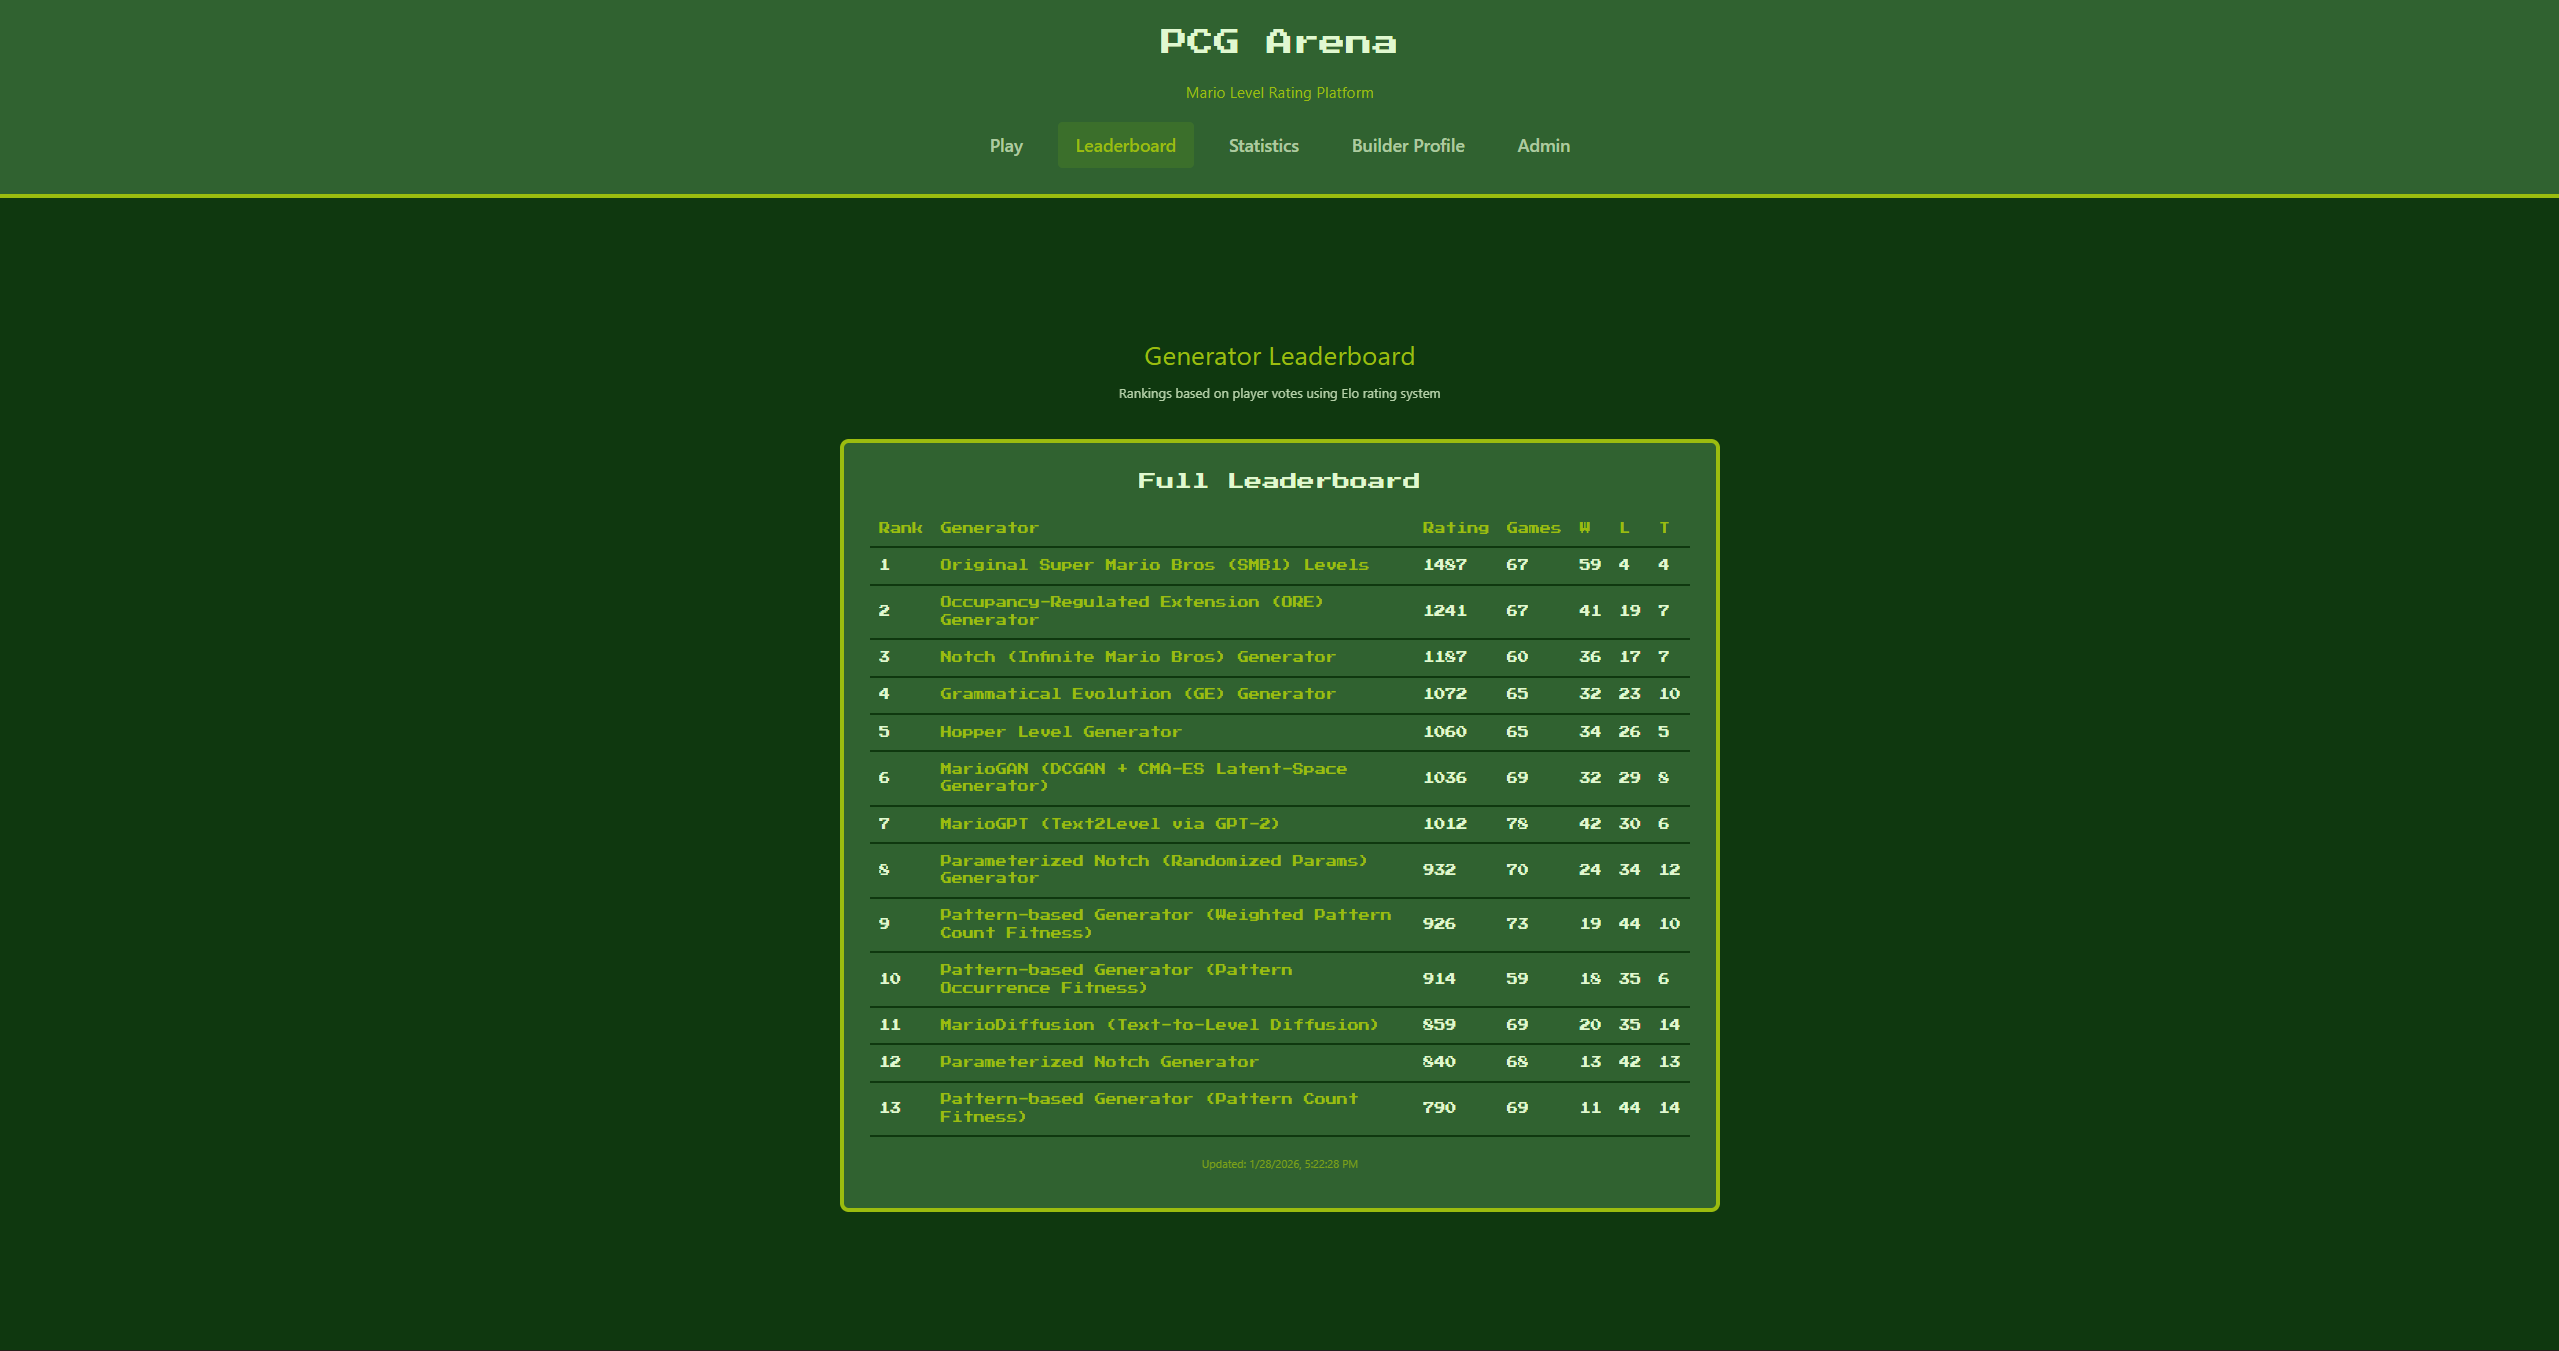
\includegraphics[width=0.95\textwidth]{leaderboard.png}
    \caption{Public leaderboard showing generator rankings with Glicko-2 ratings and uncertainty intervals.}
    \label{fig:leaderboard}
\end{figure}

The leaderboard updates in real-time as votes are submitted, allowing users to see the immediate impact of their participation.

\subsection{Generator Statistics}
\label{subsec:generator-stats}

Clicking on a generator in the leaderboard reveals detailed statistics (Figure~\ref{fig:generator-preview}):

\begin{itemize}
    \item Rating history over time
    \item Win rate against each opponent
    \item Level gallery with performance metrics per level
    \item Tag distribution (what players say about this generator's levels)
    \item Average play statistics (deaths, completion rate, time)
\end{itemize}

\begin{figure}[H]
    \centering
    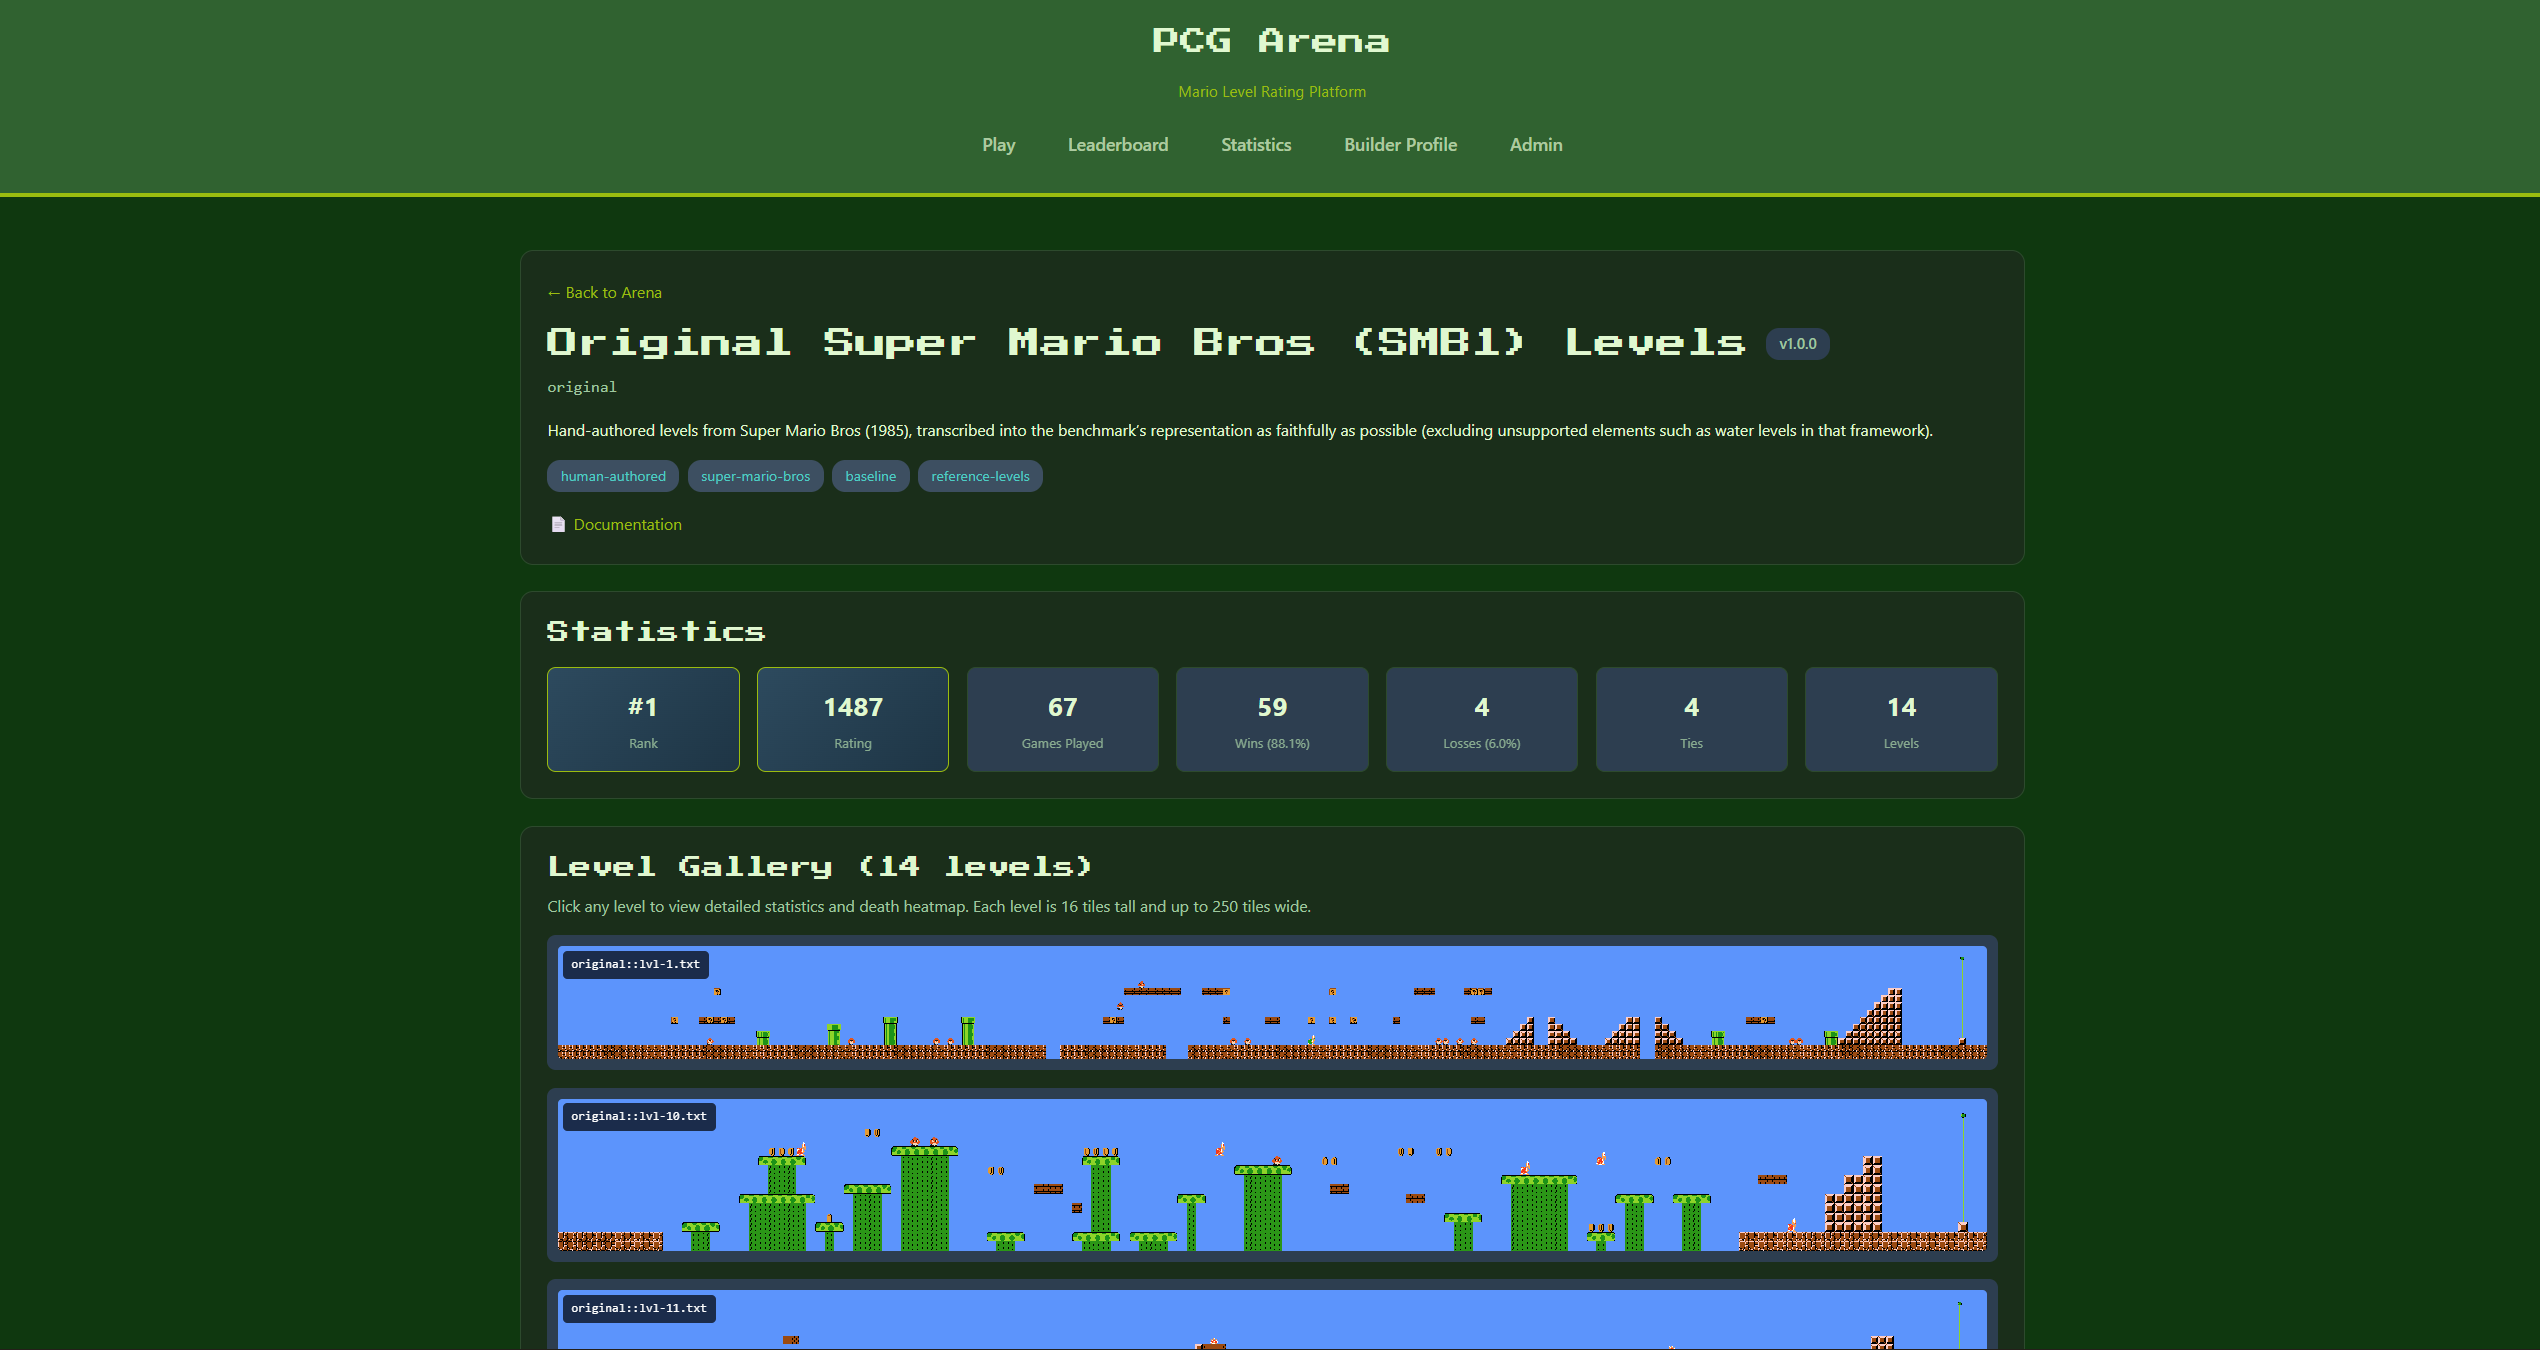
\includegraphics[width=0.95\textwidth]{generator_preview.png}
    \caption{Generator detail page showing level gallery and statistics.}
    \label{fig:generator-preview}
\end{figure}

\subsection{Confusion Matrix}
\label{subsec:confusion-matrix}

The confusion matrix (Figure~\ref{fig:confusion}) provides a comprehensive view of head-to-head performance between all generator pairs. Each cell shows the win rate when the row generator faces the column generator.

\begin{figure}[H]
    \centering
    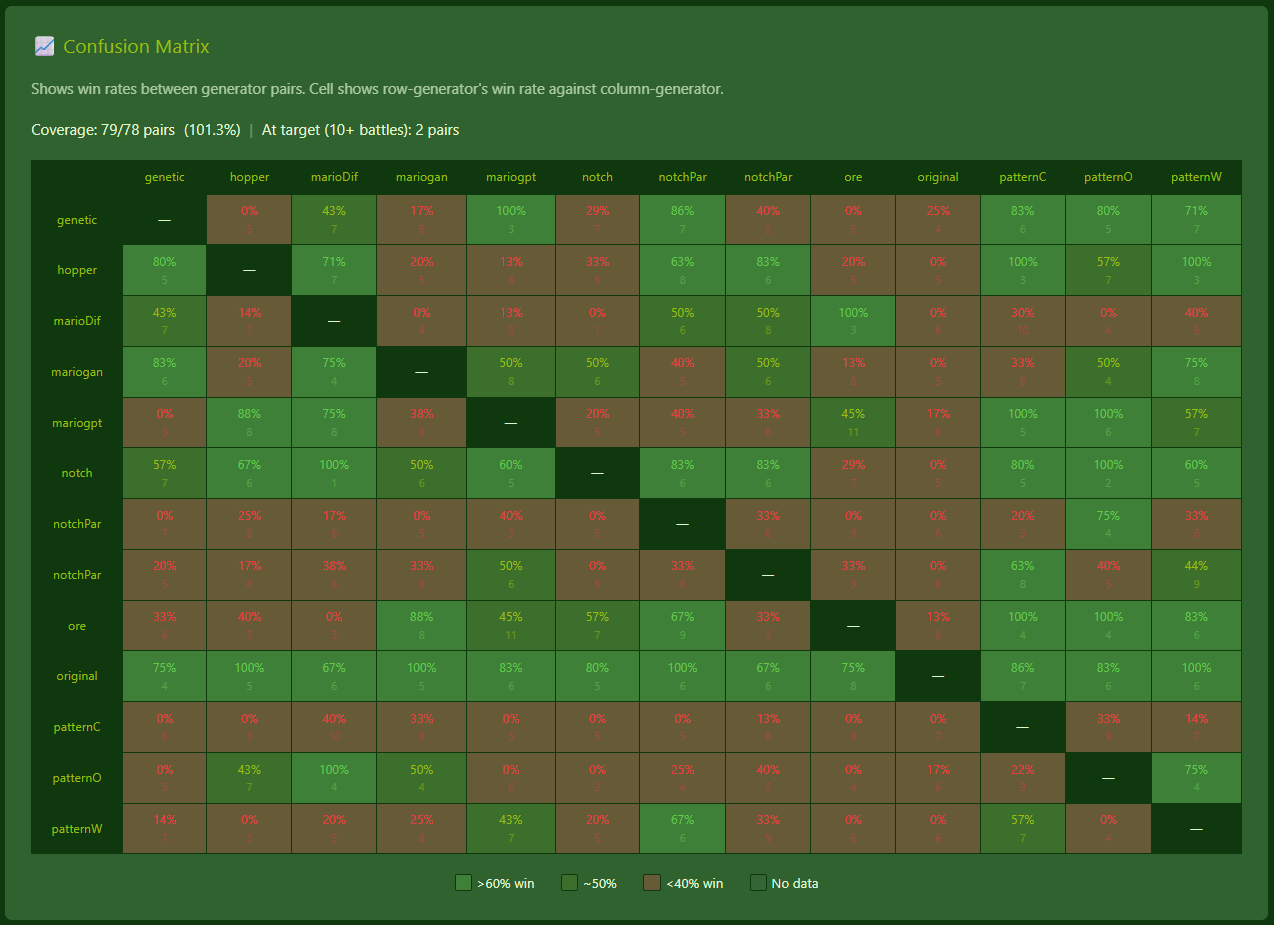
\includegraphics[width=0.8\textwidth]{confusion_matrix.png}
    \caption{Confusion matrix showing pairwise win rates between generators.}
    \label{fig:confusion}
\end{figure}

The matrix is particularly useful for:
\begin{itemize}
    \item Identifying rock-paper-scissors relationships (A beats B, B beats C, C beats A)
    \item Detecting generators with inconsistent performance
    \item Ensuring sufficient coverage---empty or low-count cells indicate gaps
\end{itemize}

Coverage gaps (Figure~\ref{fig:coverage}) are highlighted to guide future data collection.

\begin{figure}[H]
    \centering
    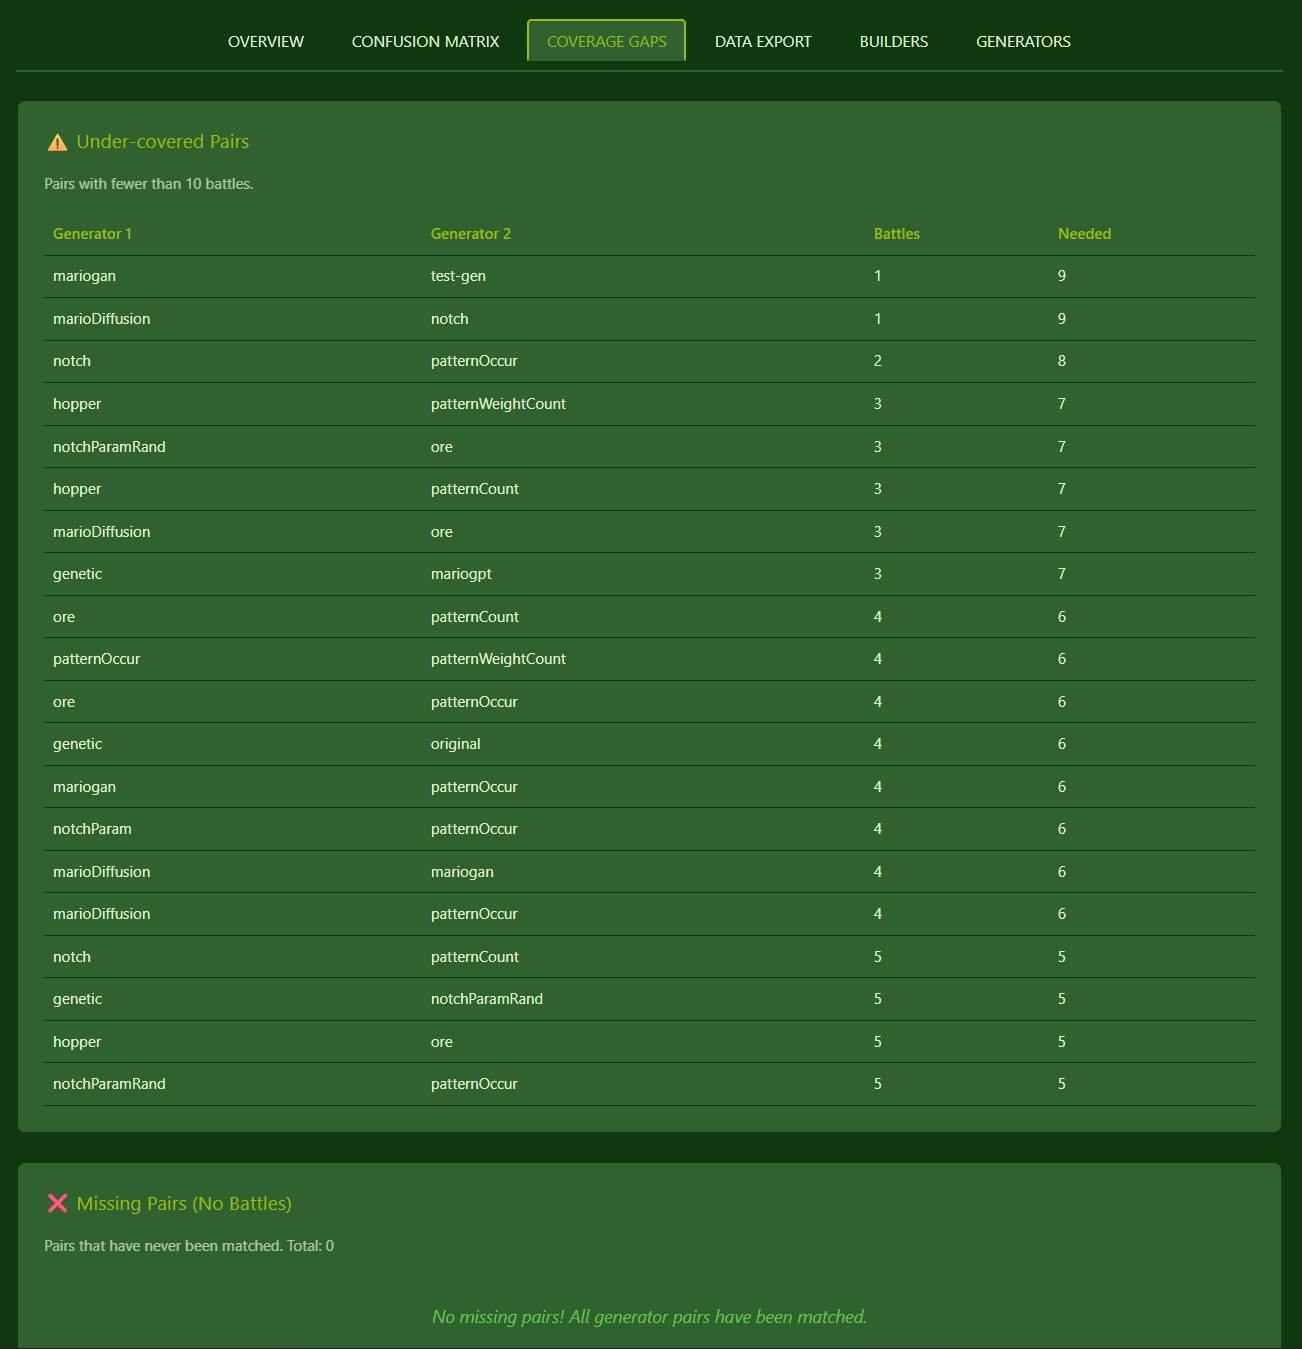
\includegraphics[width=0.8\textwidth]{coverage_gaps.png}
    \caption{Coverage analysis showing pairs with insufficient battle data.}
    \label{fig:coverage}
\end{figure}

%==============================================================================
\section{Authentication and User Management}
\label{sec:auth}
%==============================================================================

\subsection{Google OAuth Integration}
\label{subsec:google-oauth}

PCG Arena supports Google OAuth 2.0 for quick sign-in, leveraging Google's secure identity verification. The flow proceeds as:

\begin{enumerate}
    \item User clicks ``Sign In with Google''
    \item Browser opens Google OAuth popup
    \item User authenticates with Google credentials
    \item Google returns an ID token (JWT) to the frontend
    \item Frontend sends token to \texttt{POST /v1/auth/google}
    \item Backend verifies token with Google's servers
    \item Backend creates or retrieves user record
    \item Backend issues session cookie (\texttt{arena\_session})
    \item User is redirected to Builder Profile
\end{enumerate}

Google OAuth users are automatically marked as email-verified (Google handles this), enabling immediate access to submission features.

\subsection{Email/Password Authentication}
\label{subsec:email-auth}

For users who prefer not to use Google, PCG Arena supports traditional email/password authentication:

\textbf{Registration:}
\begin{enumerate}
    \item User provides email, password, and display name
    \item Backend validates email format and password strength
    \item Password is hashed using bcrypt (work factor 12)
    \item User record created with \texttt{is\_email\_verified = 0}
    \item Verification email sent (see Section~\ref{subsec:email-verification})
\end{enumerate}

\textbf{Login:}
\begin{enumerate}
    \item User provides email and password
    \item Backend retrieves user record by email
    \item Password verified against stored hash
    \item Session cookie issued on successful verification
\end{enumerate}

Security measures include:
\begin{itemize}
    \item Password minimum length: 8 characters
    \item Session tokens: 256-bit cryptographically random
    \item Session expiry: 7 days (configurable)
    \item HTTP-only cookies prevent XSS token theft
\end{itemize}

\subsection{Email Verification with Twilio SendGrid}
\label{subsec:email-verification}

Email verification ensures that users control the email addresses they register with. PCG Arena uses Twilio SendGrid for email delivery:

\begin{enumerate}
    \item On registration, generate a random verification token (64 hex characters)
    \item Store token in \texttt{email\_verifications} table with 24-hour expiry
    \item Send verification email via SendGrid API containing link: \\ \texttt{https://pcg-arena.com/verify-email?token=<token>}
    \item User clicks link, frontend calls \texttt{POST /v1/auth/verify-email}
    \item Backend verifies token validity and expiry
    \item User marked as verified; token deleted
\end{enumerate}

Password reset follows a similar flow, using separate tokens stored in \texttt{password\_resets}. Reset tokens expire after 1 hour for security.

%==============================================================================
\section{Builder Profile}
\label{sec:builder}
%==============================================================================

\subsection{Generator Submission}
\label{subsec:generator-submission}

The Builder Profile (Figure~\ref{fig:builder}) enables authenticated researchers to submit their own generators to compete on the leaderboard. The submission process:

\begin{enumerate}
    \item User navigates to Builder Profile (requires authentication)
    \item Fills out generator metadata: name, version, description, tags, URL
    \item Uploads a ZIP file containing level files (ASCII tilemaps)
    \item Backend validates all levels (see Section~\ref{subsec:level-validation})
    \item Generator and levels are inserted into the database
    \item Initial Glicko-2 rating assigned (1000 $\pm$ 350)
    \item Generator appears on leaderboard immediately
\end{enumerate}

\begin{figure}[H]
    \centering
    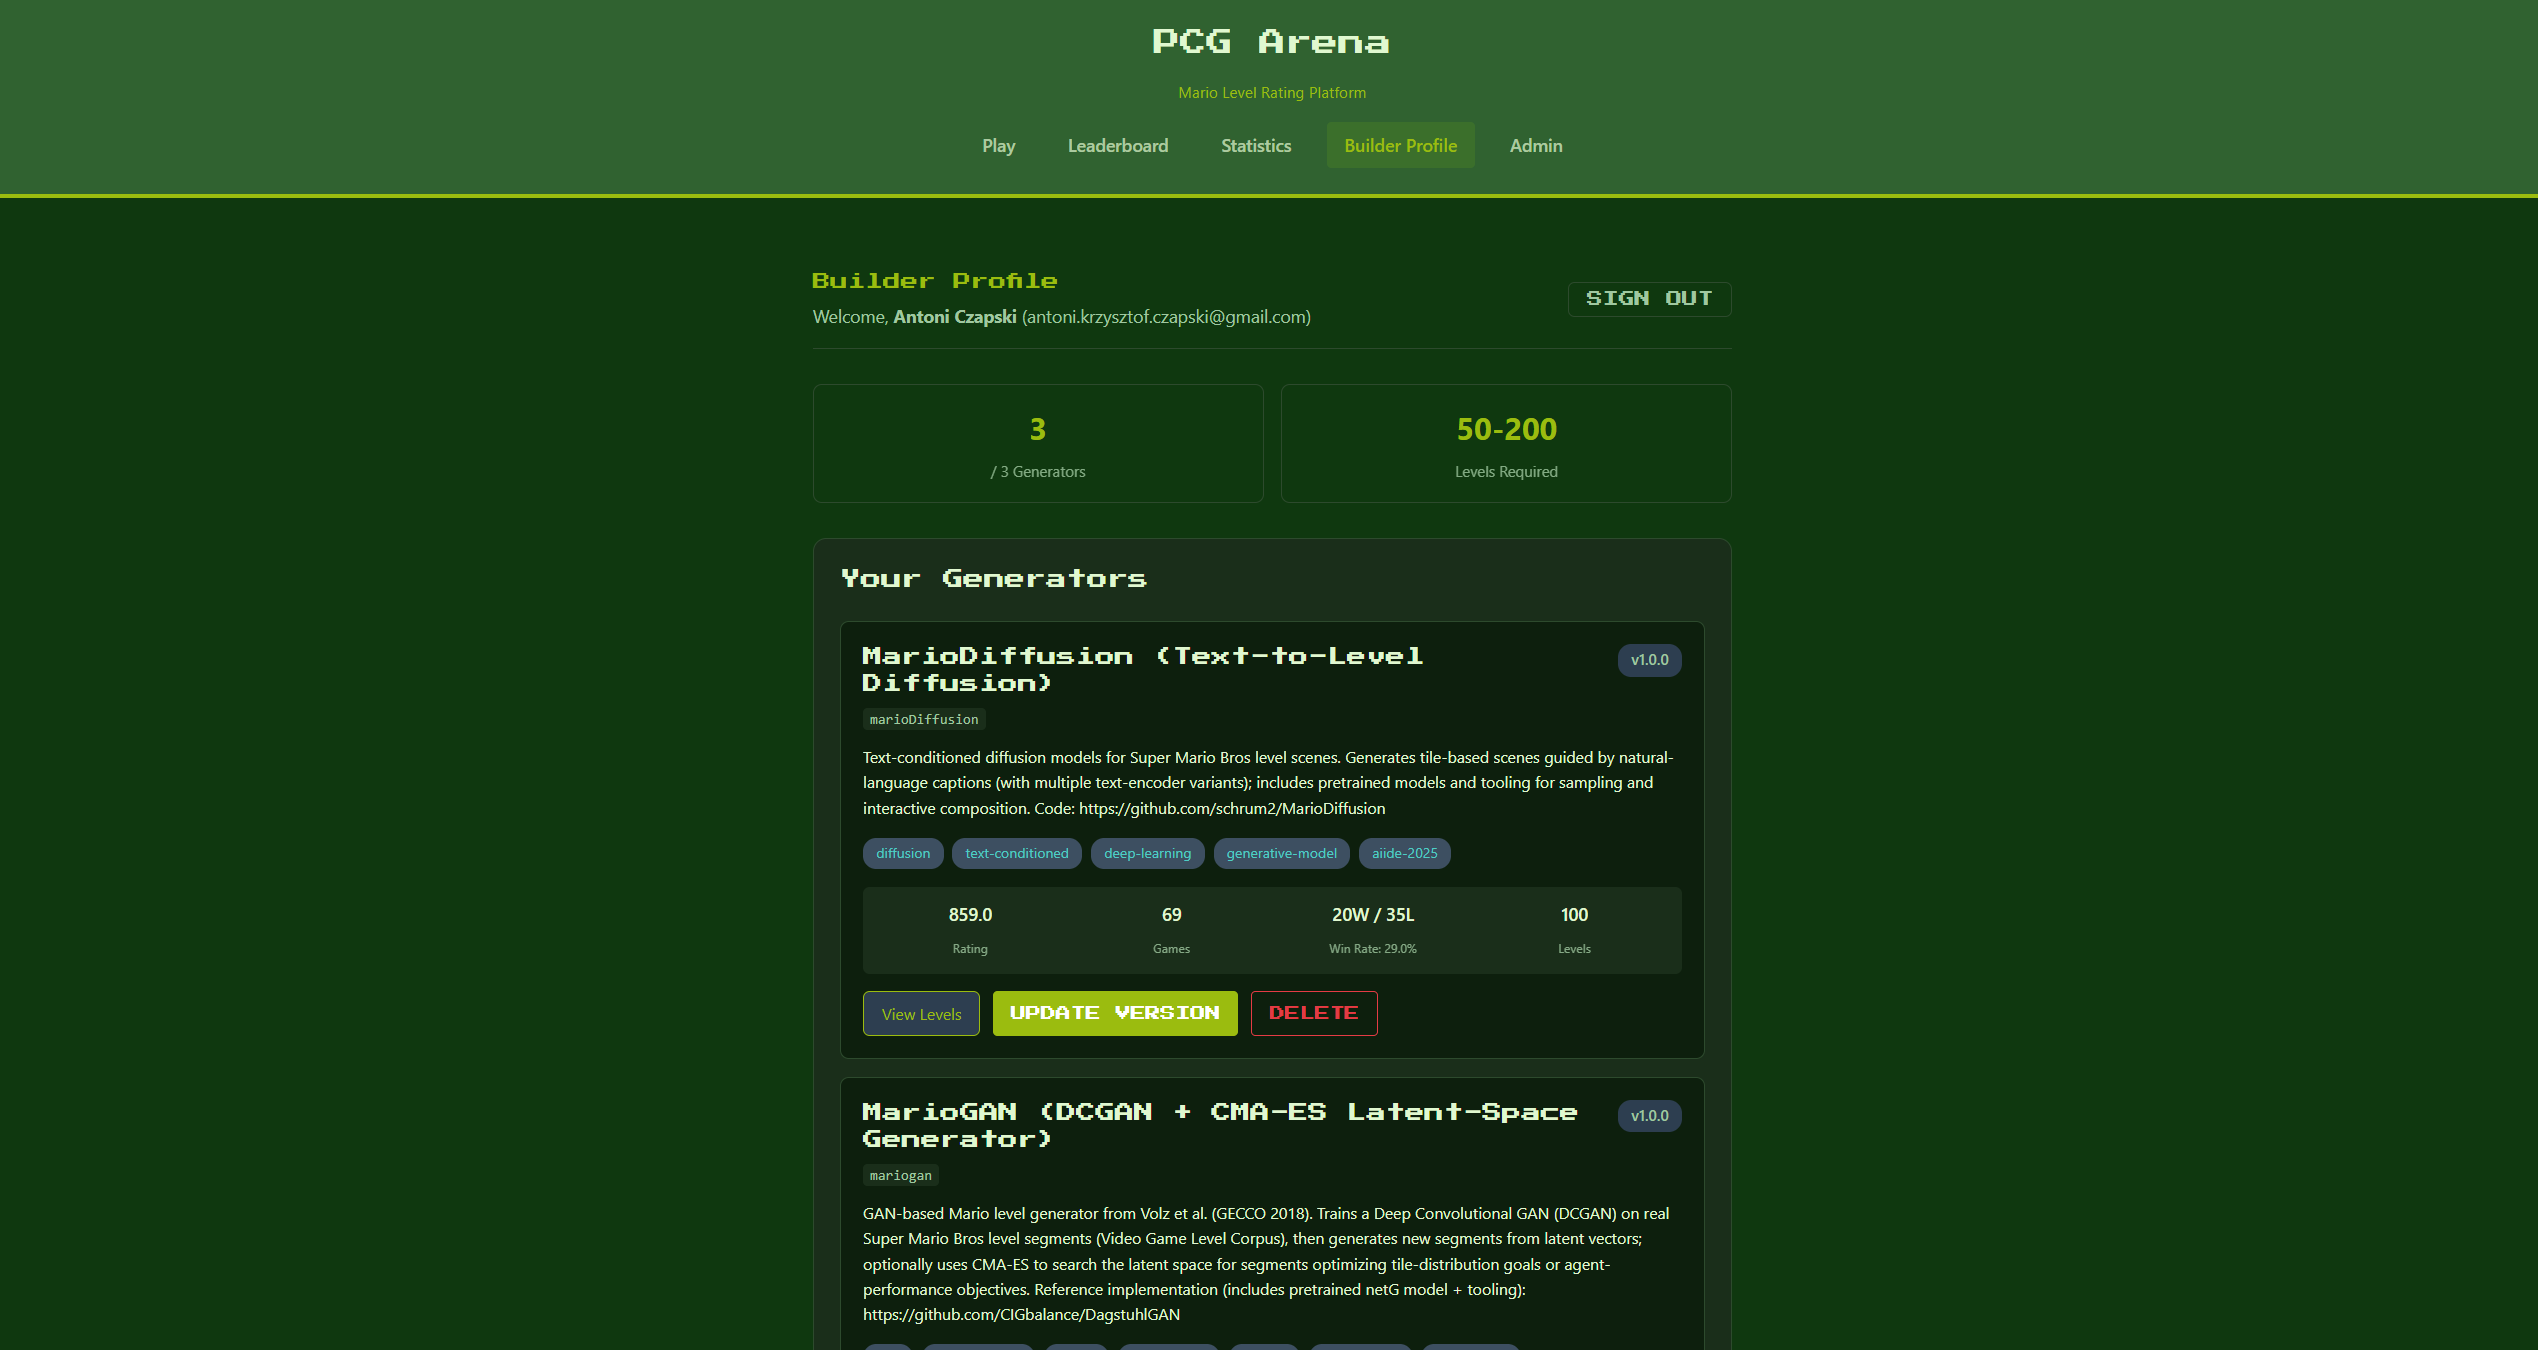
\includegraphics[width=0.95\textwidth]{builder_profile.png}
    \caption{Builder Profile page for managing submitted generators.}
    \label{fig:builder}
\end{figure}

Constraints on submissions:
\begin{itemize}
    \item Maximum 3 generators per user (prevents flooding)
    \item 50--200 levels per generator (ensures variety without overwhelming)
    \item Each level must pass validation checks
\end{itemize}

\subsection{Level Validation}
\label{subsec:level-validation}

Every submitted level undergoes validation to ensure playability:

\begin{enumerate}
    \item \textbf{Format Check}: File must be valid ASCII, correct dimensions
    \item \textbf{Character Validation}: Only recognized tile characters allowed
    \item \textbf{Spawn/Exit Check}: Level must have Mario spawn point and reachable exit
    \item \textbf{Deduplication}: Content hash computed; duplicates rejected
    \item \textbf{Playability Heuristics}: Basic reachability analysis
\end{enumerate}

Validation errors return detailed feedback indicating which levels failed and why, enabling researchers to fix issues before resubmitting.

\subsection{Generator Management}
\label{subsec:generator-management}

After submission, researchers can manage their generators:

\textbf{Update Version:}
\begin{itemize}
    \item Upload new level set while preserving rating
    \item Version number incremented
    \item Old levels replaced with new ones
    \item Rating history maintained for continuity
\end{itemize}

\textbf{Delete Generator:}
\begin{itemize}
    \item Generators with battles: soft delete (marked inactive, preserved for historical data)
    \item Generators without battles: hard delete (completely removed)
    \item Soft-deleted generators don't appear in matchmaking but remain in historical rankings
\end{itemize}

This design ensures data integrity---votes referencing deleted generators remain valid for research analysis.

%==============================================================================
\section{Admin Dashboard}
\label{sec:admin}
%==============================================================================

\subsection{Platform Overview}
\label{subsec:admin-overview}

The Admin Dashboard (Figure~\ref{fig:admin-dashboard}) provides platform administrators with comprehensive oversight and management capabilities. Access is restricted to users whose email addresses are listed in the \texttt{ARENA\_ADMIN\_EMAILS} configuration.

\begin{figure}[H]
    \centering
    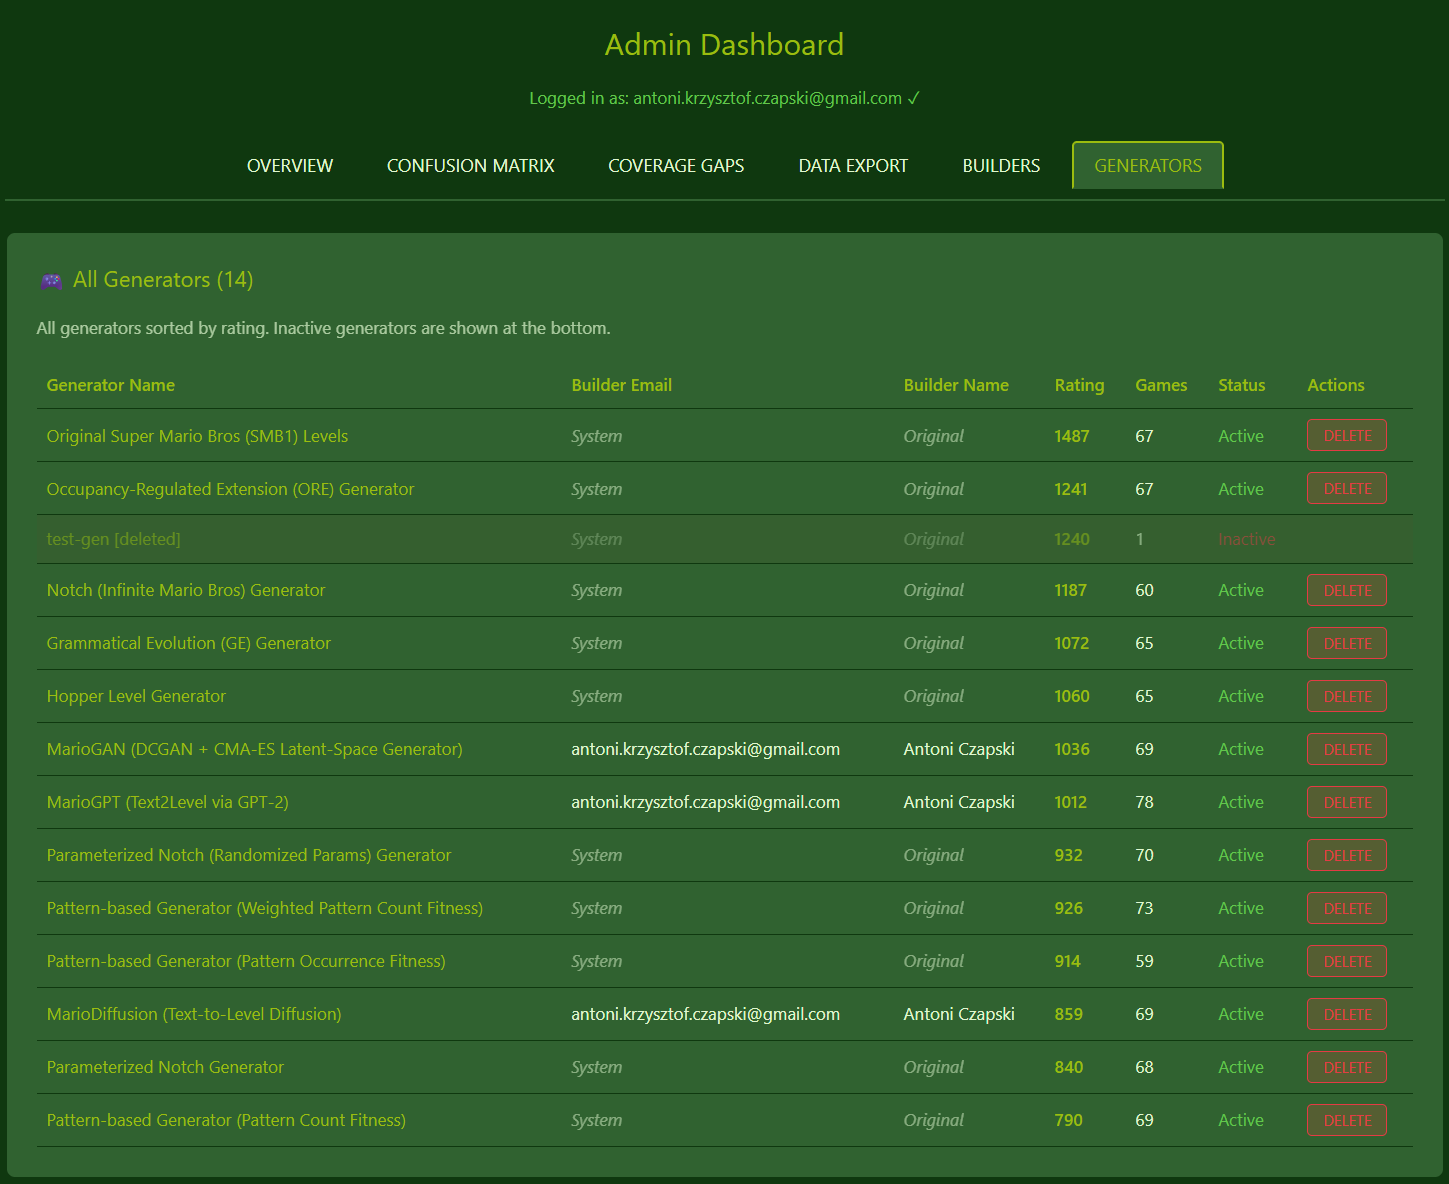
\includegraphics[width=0.95\textwidth]{admin_dashboard.png}
    \caption{Admin Dashboard showing platform statistics and management tools.}
    \label{fig:admin-dashboard}
\end{figure}

Key metrics displayed:
\begin{itemize}
    \item Total battles completed and pending
    \item Total votes and vote distribution (left/right/tie/skip)
    \item Active generators and users
    \item Recent activity timeline
    \item System health indicators
\end{itemize}

Administrative actions available:
\begin{itemize}
    \item View and ban builder accounts
    \item Delete inappropriate generators
    \item Monitor matchmaking statistics
    \item Trigger manual data exports
\end{itemize}

\subsection{Data Export}
\label{subsec:data-export}

PCG Arena provides comprehensive data export for research purposes (Figure~\ref{fig:data-export}). Export endpoints (admin-only) include:

\begin{table}[H]
\centering
\begin{tabular}{ll}
\toprule
\textbf{Endpoint} & \textbf{Data} \\
\midrule
\texttt{/v1/admin/export/votes} & All votes with telemetry and tags \\
\texttt{/v1/admin/export/trajectories} & Player position traces \\
\texttt{/v1/admin/export/level-stats} & Aggregate per-level metrics \\
\texttt{/v1/admin/export/player-profiles} & Anonymous player IDs and sessions \\
\bottomrule
\end{tabular}
\caption{Available data export endpoints.}
\label{tab:exports}
\end{table}

\begin{figure}[H]
    \centering
    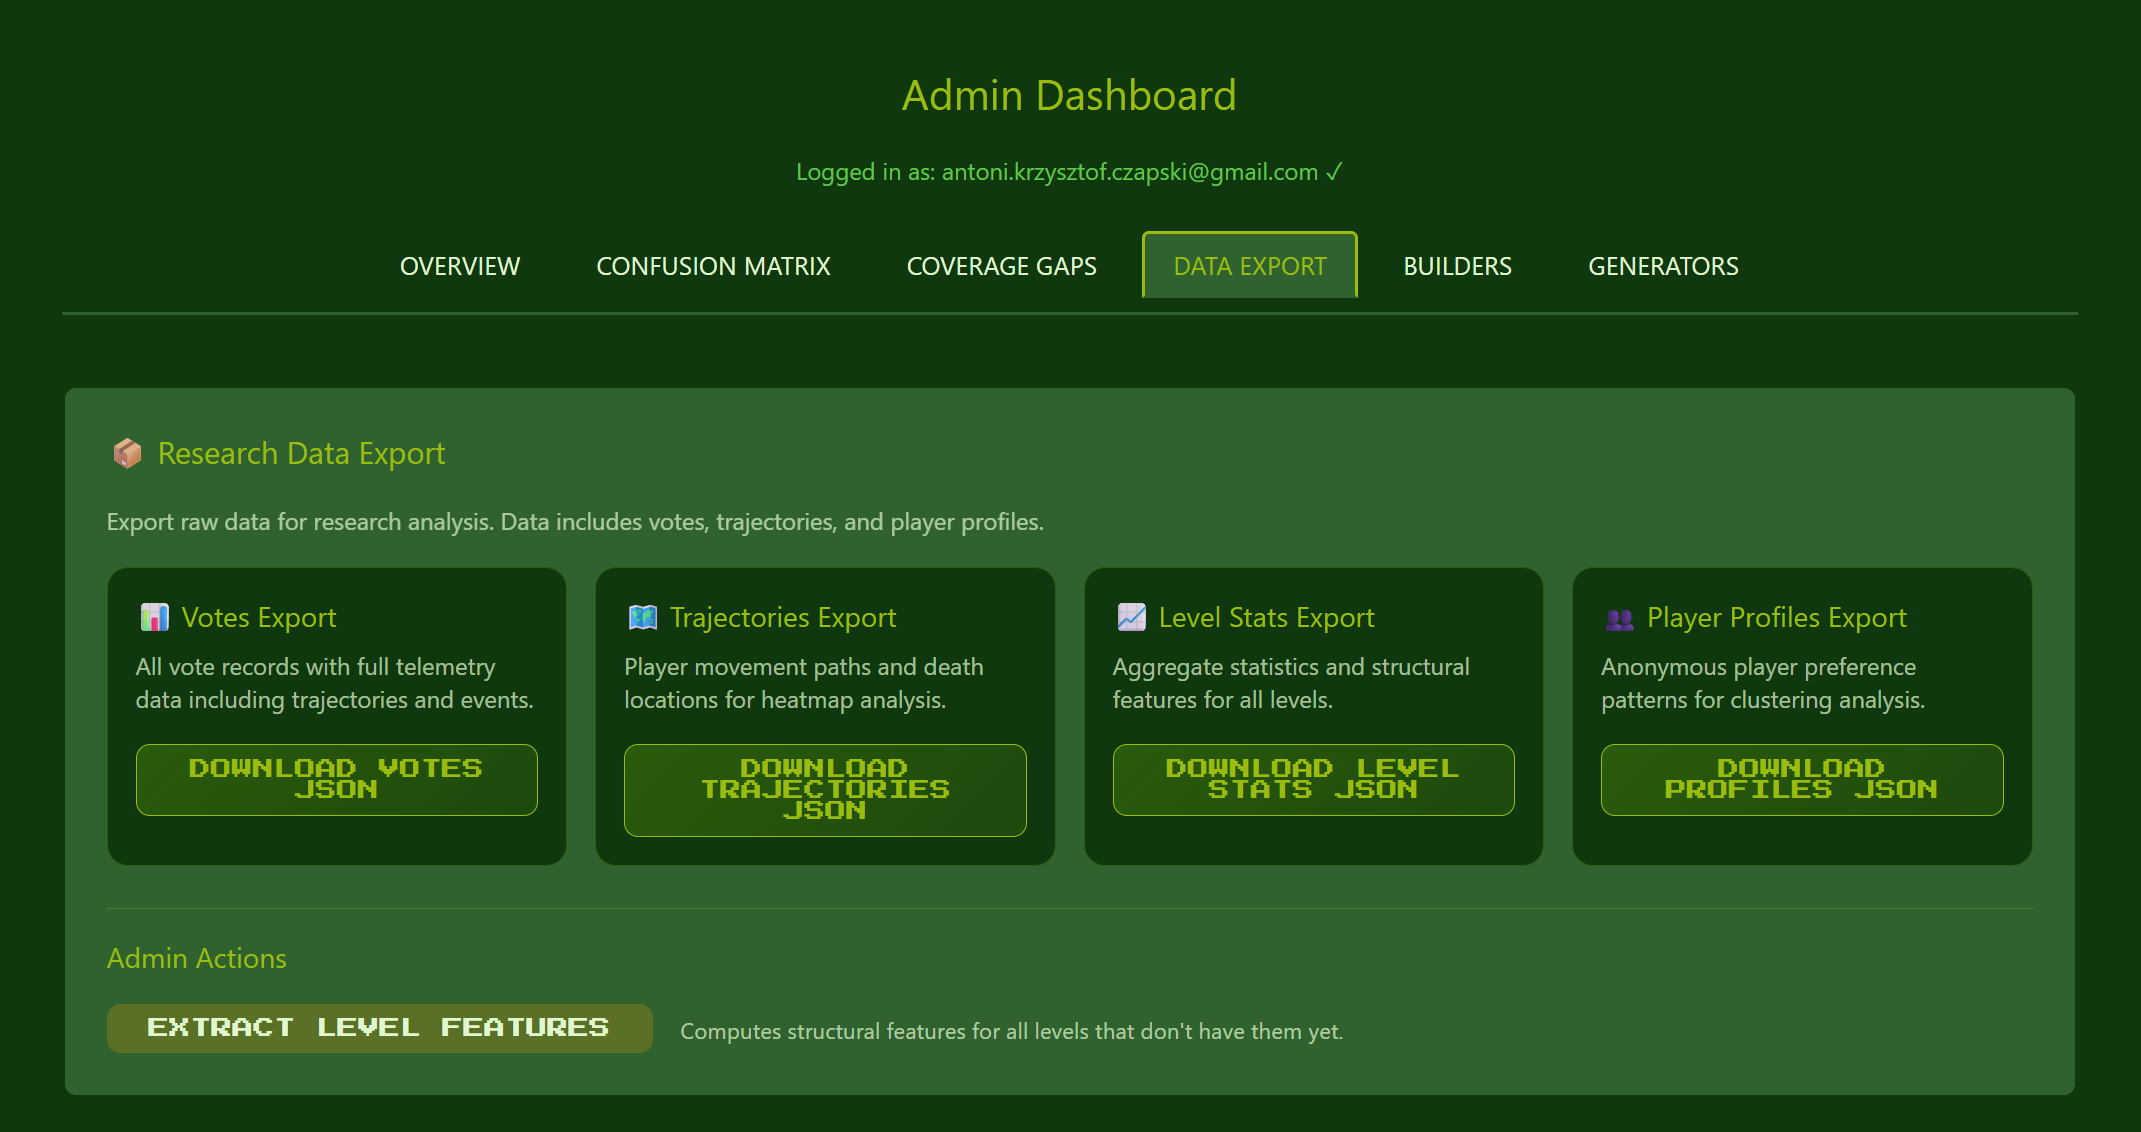
\includegraphics[width=0.9\textwidth]{data_export.png}
    \caption{Data export interface for downloading research datasets.}
    \label{fig:data-export}
\end{figure}

Data is exported in JSON and CSV formats suitable for analysis with standard tools (Python/pandas, R, etc.).

\subsection{Research Analytics}
\label{subsec:research-analytics}

The platform collects rich telemetry enabling advanced research analytics:

\textbf{Level Statistics} (Figure~\ref{fig:statistics}):
\begin{itemize}
    \item Completion rate: percentage of players who finish
    \item Death rate: average deaths per attempt
    \item Average play time
    \item Win rate when featured in battles
\end{itemize}

\begin{figure}[H]
    \centering
    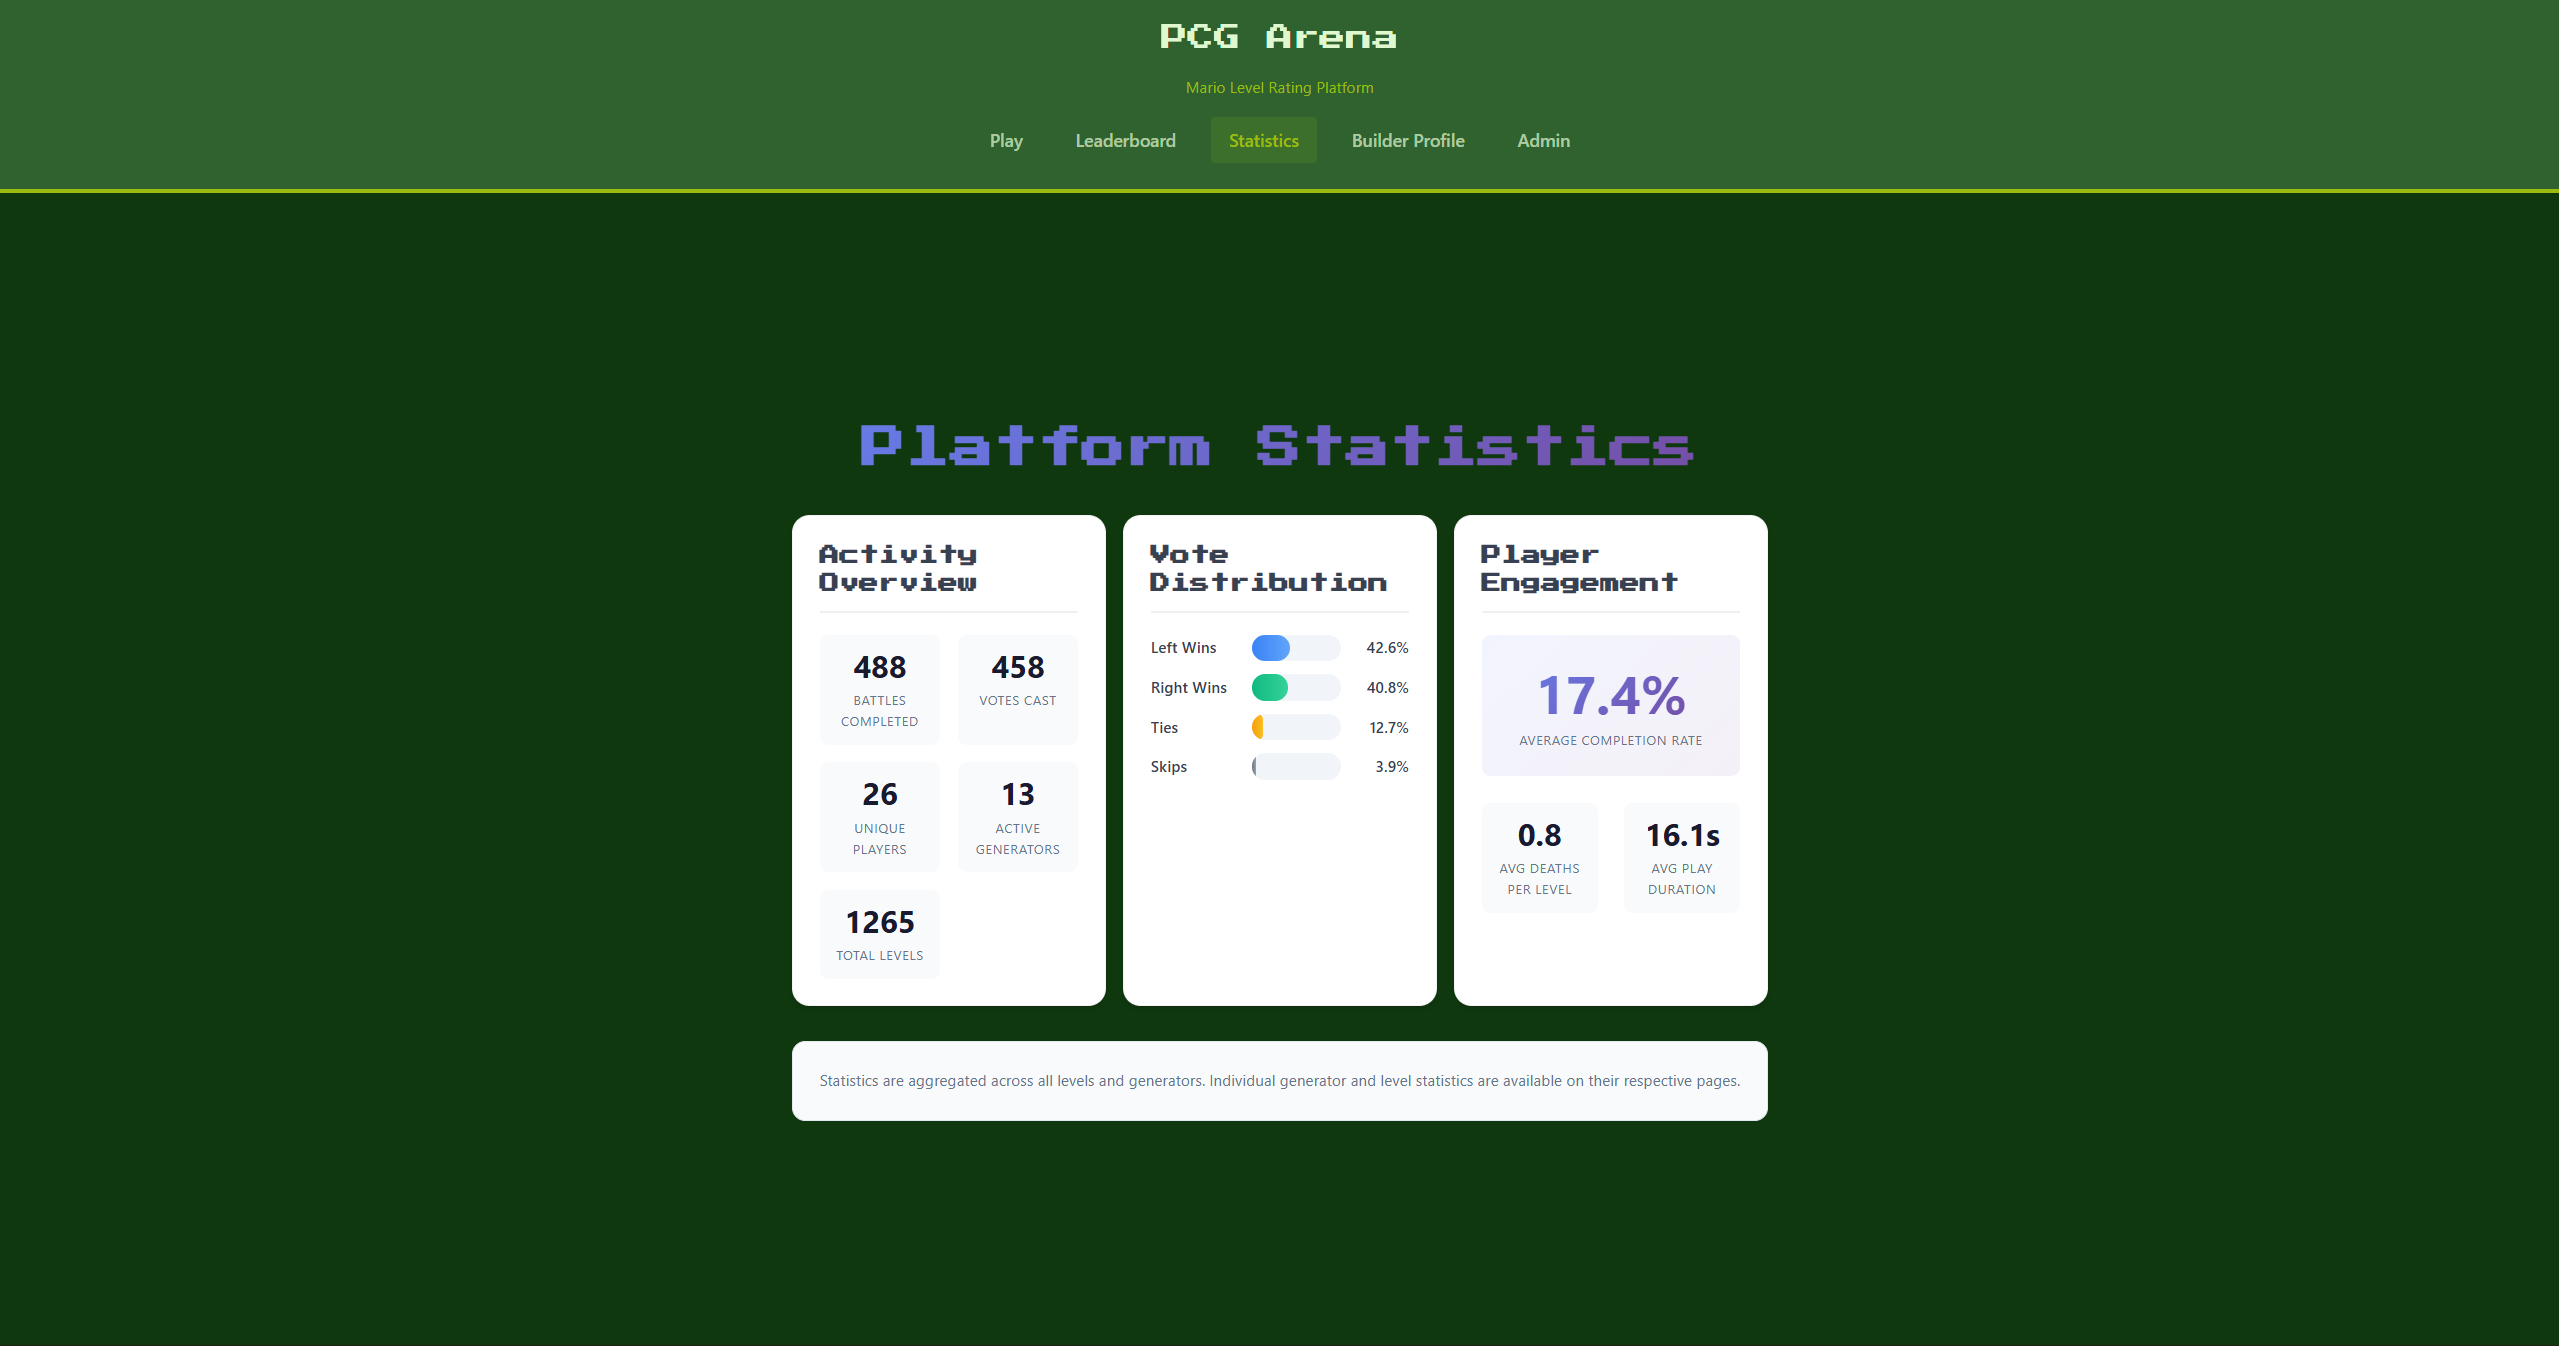
\includegraphics[width=0.95\textwidth]{statistics_page.png}
    \caption{Statistics page showing detailed level and generator analytics.}
    \label{fig:statistics}
\end{figure}

\textbf{Death Heatmaps}:
\begin{itemize}
    \item Aggregate death locations across all plays of a level
    \item Reveals difficulty spikes and design issues
    \item Exportable for external visualization
\end{itemize}

\textbf{Detailed Level View} (Figure~\ref{fig:detailed-level}):
\begin{itemize}
    \item Full level visualization with overlay options
    \item Play trajectory visualization
    \item Per-tile analysis
\end{itemize}

\begin{figure}[H]
    \centering
    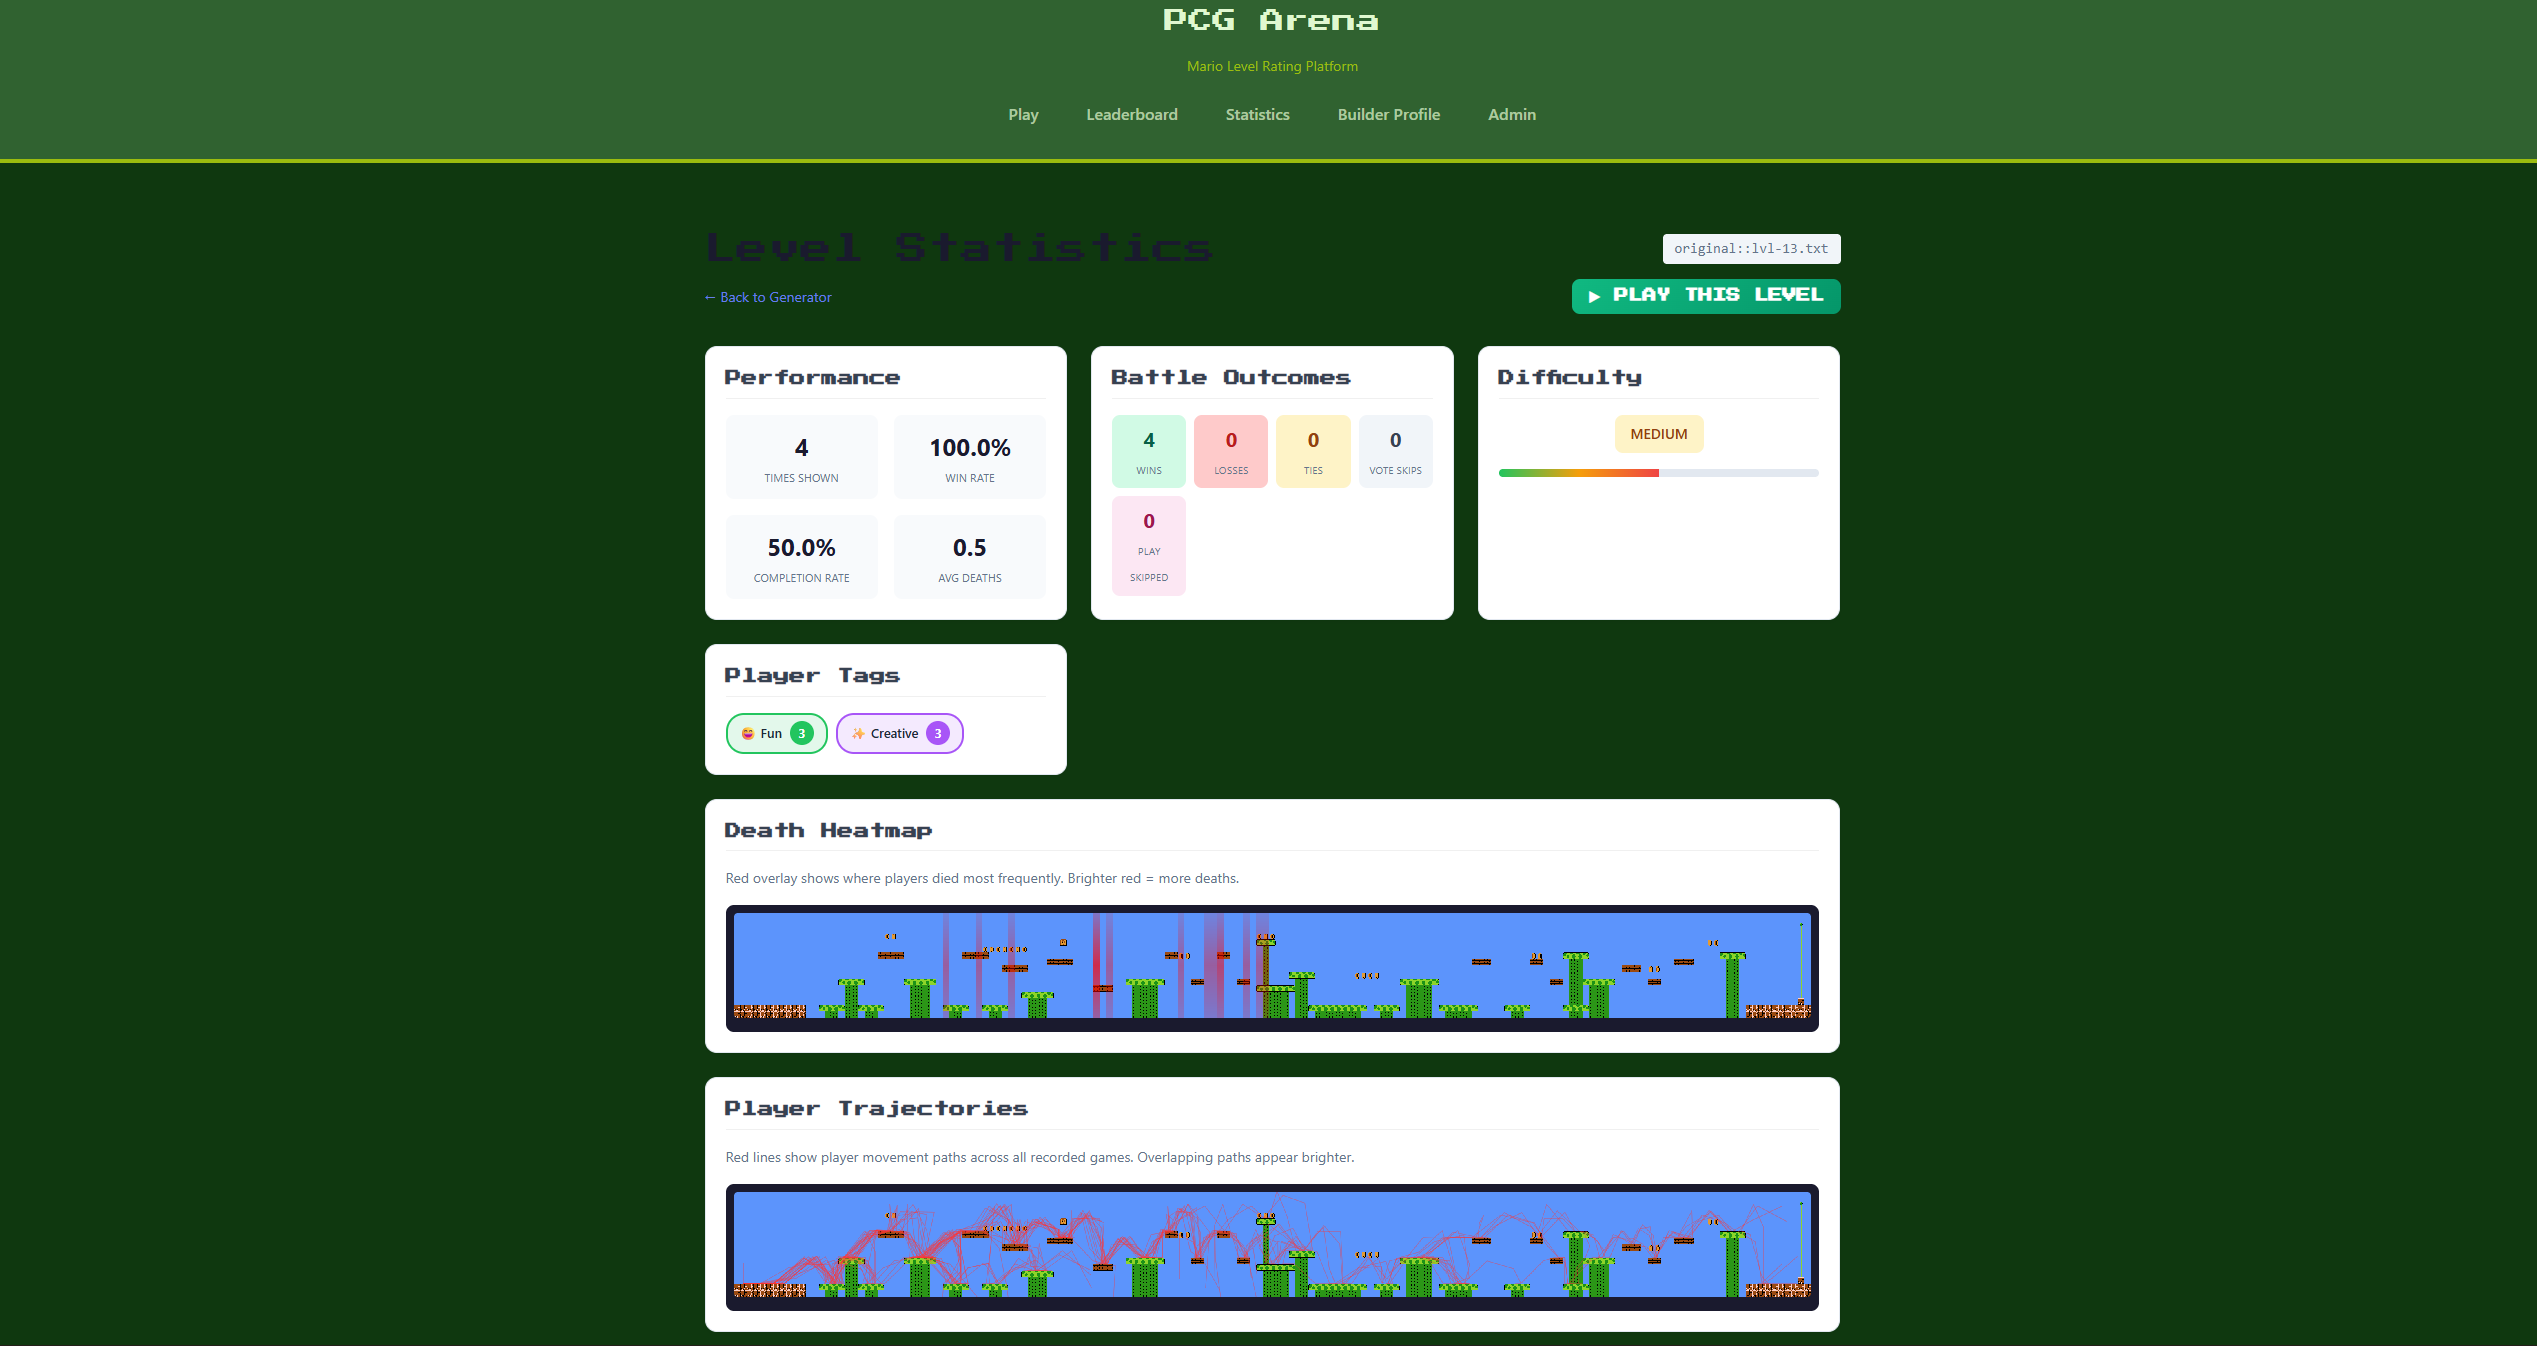
\includegraphics[width=0.95\textwidth]{detailed_level_view.png}
    \caption{Detailed level view with analytics overlays.}
    \label{fig:detailed-level}
\end{figure}

%==============================================================================
\section{Deployment and Infrastructure}
\label{sec:deployment}
%==============================================================================

\subsection{Google Cloud Platform Setup}
\label{subsec:gcp}

PCG Arena is deployed on Google Cloud Platform (GCP) using a single Compute Engine virtual machine. This setup balances cost-effectiveness with reliability for a research platform:

\textbf{VM Specifications:}
\begin{itemize}
    \item Machine type: \texttt{e2-micro} (free tier eligible)
    \item Region: \texttt{us-central1} (low latency for most users)
    \item Boot disk: Ubuntu 22.04 LTS, 10 GB standard persistent disk
    \item Static external IP: reserved for DNS stability
\end{itemize}

\textbf{Firewall Configuration:}
\begin{itemize}
    \item Port 80 (HTTP): Allowed for redirect to HTTPS
    \item Port 443 (HTTPS): Allowed for all traffic
    \item Port 8080 (backend): \textbf{NOT} public; backend binds to localhost
\end{itemize}

The architecture ensures that all public traffic goes through the Caddy reverse proxy, which handles TLS termination and routes requests appropriately.

\subsection{Docker Containerization}
\label{subsec:docker}

The backend runs in a Docker container, providing:

\begin{itemize}
    \item Consistent environment across development and production
    \item Easy deployment via \texttt{docker compose up -d --build}
    \item Isolated dependencies (Python packages)
    \item Simple rollback by switching image tags
\end{itemize}

The \texttt{docker-compose.yml} configuration:

\begin{lstlisting}[language=bash]
services:
  backend:
    build: ./backend
    ports:
      - "127.0.0.1:8080:8080"  # Localhost only
    volumes:
      - ./db/local:/data
      - ./db/migrations:/migrations
      - ./db/seed:/seed
    environment:
      - ARENA_DB_PATH=/data/arena.sqlite
\end{lstlisting}

Database files are bind-mounted from the host, ensuring persistence across container rebuilds.

\subsection{Domain and HTTPS Configuration}
\label{subsec:domain}

The platform is accessible at \url{https://pcg-arena.com}, configured as follows:

\textbf{Domain Registration:}
\begin{itemize}
    \item Domain: \texttt{pcg-arena.com} (registered via Namecheap)
    \item DNS A records: \texttt{@} and \texttt{www} point to VM's static IP
\end{itemize}

\textbf{HTTPS via Caddy:}
\begin{itemize}
    \item Automatic TLS certificate provisioning (Let's Encrypt)
    \item Automatic certificate renewal
    \item HTTP to HTTPS redirect
    \item Reverse proxy to backend (\texttt{localhost:8080})
    \item Static file serving for frontend build
\end{itemize}

Caddyfile configuration:

\begin{lstlisting}
pcg-arena.com, www.pcg-arena.com {
    root * /var/www/pcg-arena/frontend/dist
    file_server
    
    @api path /v1/* /health
    handle @api {
        reverse_proxy localhost:8080
    }
    
    try_files {path} /index.html
}
\end{lstlisting}

\subsection{Monitoring and Alerts}
\label{subsec:monitoring}

GCP provides built-in monitoring capabilities:

\begin{itemize}
    \item \textbf{Uptime Checks}: HTTP(S) probe to \texttt{/health} endpoint every 60 seconds
    \item \textbf{Alerting Policies}: Email notification when health check fails
    \item \textbf{VM Metrics}: CPU, memory, disk usage monitoring
    \item \textbf{Logging}: Application logs accessible via Cloud Console
\end{itemize}

Automated backups run daily via cron job:
\begin{lstlisting}[language=bash]
0 3 * * * /home/user/pcg-arena/backend/scripts/backup.sh
\end{lstlisting}

Backups are stored in \texttt{/backups/} with 7-day retention, enabling recovery from data corruption or accidental deletion.

%==============================================================================
\section{Results and Discussion}
\label{sec:results}
%==============================================================================

This section presents the results of exploratory data analysis conducted on the PCG Arena platform data. The analysis investigates three research questions: (1) what makes a good generator/level, (2) whether players are consistent in their preferences, and (3) what player-assigned tags actually mean in terms of measurable gameplay differences.

\subsection{Dataset Overview}
\label{subsec:dataset-overview}

The analysis encompasses data collected from the live platform:

\begin{table}[H]
\centering
\caption{Dataset Summary}
\label{tab:dataset-summary}
\begin{tabular}{lr}
\toprule
\textbf{Category} & \textbf{Count} \\
\midrule
Levels & 631 \\
Generators & 14 \\
Total Votes & 447 \\
Players & 26 \\
Telemetry Records & 894 \\
Trajectory Samples & 100 \\
\bottomrule
\end{tabular}
\end{table}

Key global statistics include: mean win rate of 0.47 (slightly below 50\%, indicating some generators are notably worse), mean death rate of 0.80 deaths per play, mean completion rate of only 18\%, and average play duration of 17.7 seconds.

\begin{figure}[H]
\centering
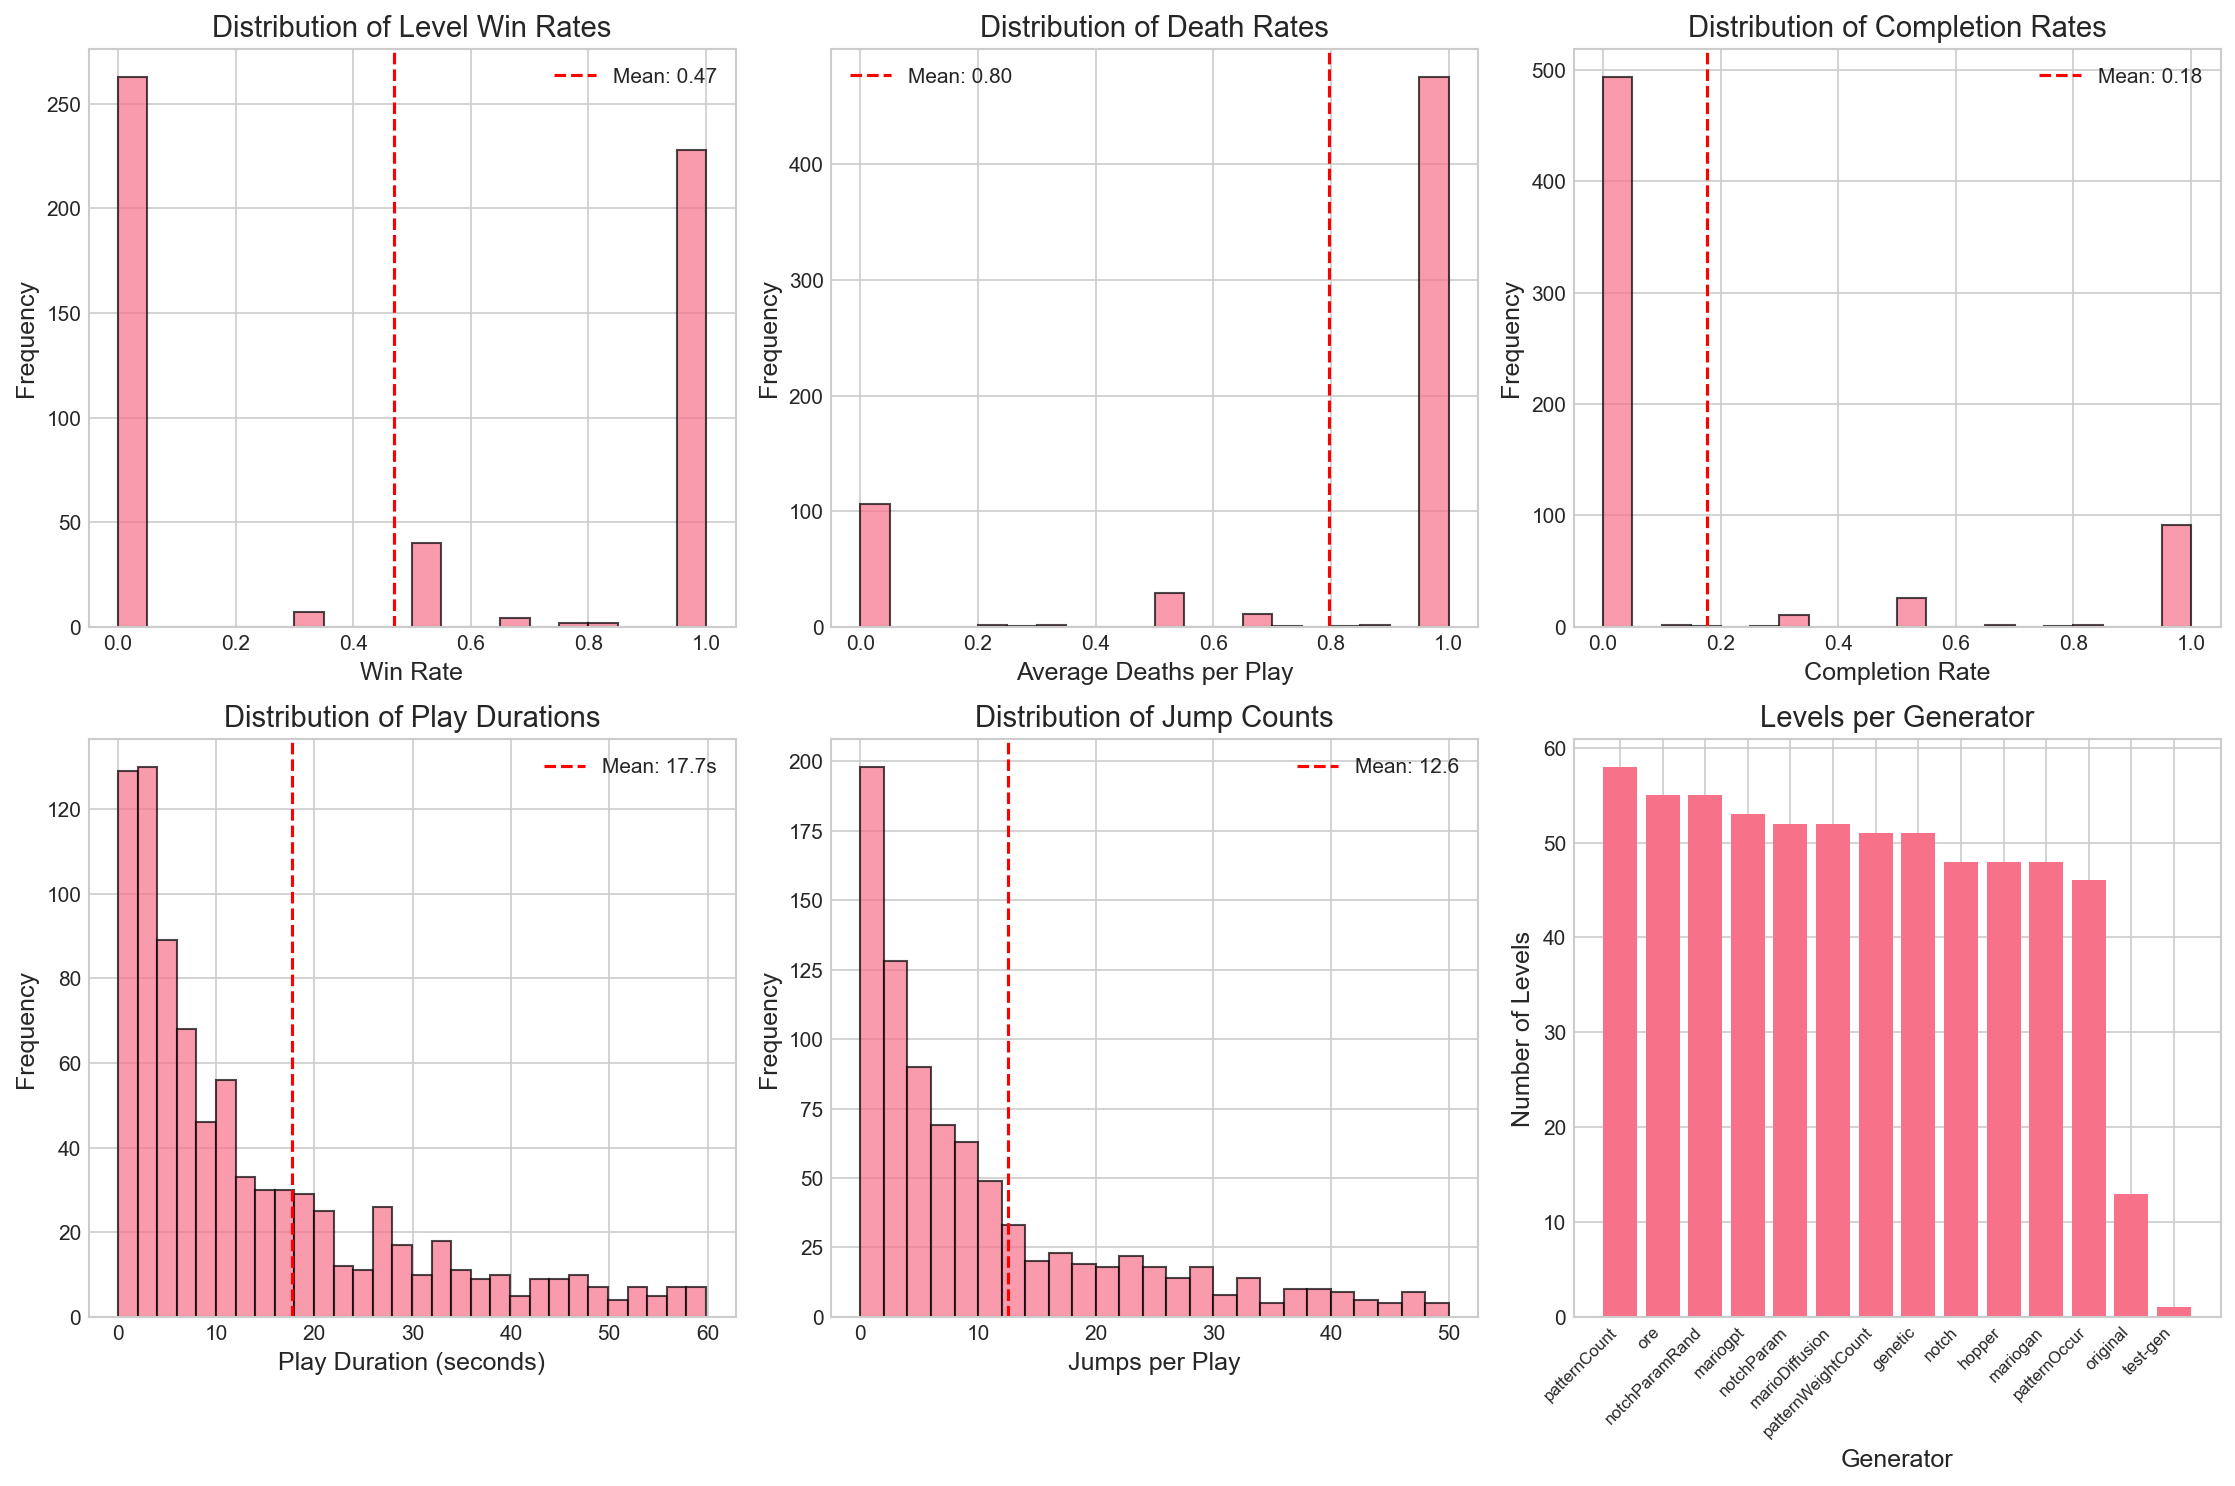
\includegraphics[width=\textwidth]{global_distributions.png}
\caption{Global distributions of key platform metrics: win rates, death rates, completion rates, play durations, jump counts, and levels per generator.}
\label{fig:global-distributions}
\end{figure}

\subsection{Generator Rankings and Performance}
\label{subsec:generator-rankings}

Analysis of generator performance reveals substantial quality differences across the 14 generators tested. Table~\ref{tab:generator-rankings} presents the top and bottom performers by win rate.

\begin{table}[H]
\centering
\caption{Generator Performance Rankings}
\label{tab:generator-rankings}
\begin{tabular}{llrrr}
\toprule
\textbf{Rank} & \textbf{Generator} & \textbf{Win Rate} & \textbf{Avg Deaths} & \textbf{Completion Rate} \\
\midrule
1 & original & 92.5\% & 0.73 & 27.5\% \\
2 & ore & 67.8\% & 0.85 & 14.2\% \\
3 & notch & 67.5\% & 0.69 & 31.3\% \\
4 & mariogpt & 62.4\% & 0.72 & 19.8\% \\
5 & hopper & 58.7\% & 0.76 & 24.0\% \\
\midrule
12 & patternWeightCount & 25.9\% & 0.90 & 6.2\% \\
13 & notchParam & 22.1\% & 0.83 & 17.0\% \\
14 & patternCount & 22.0\% & 0.93 & 2.3\% \\
\bottomrule
\end{tabular}
\end{table}

The hand-crafted ``original'' levels dominate with a 92.5\% win rate, serving as the benchmark. Among procedural generators, ``ore'' and ``notch'' perform best (67-68\%), while pattern-based generators consistently rank at the bottom ($<$26\%).

\begin{figure}[H]
\centering
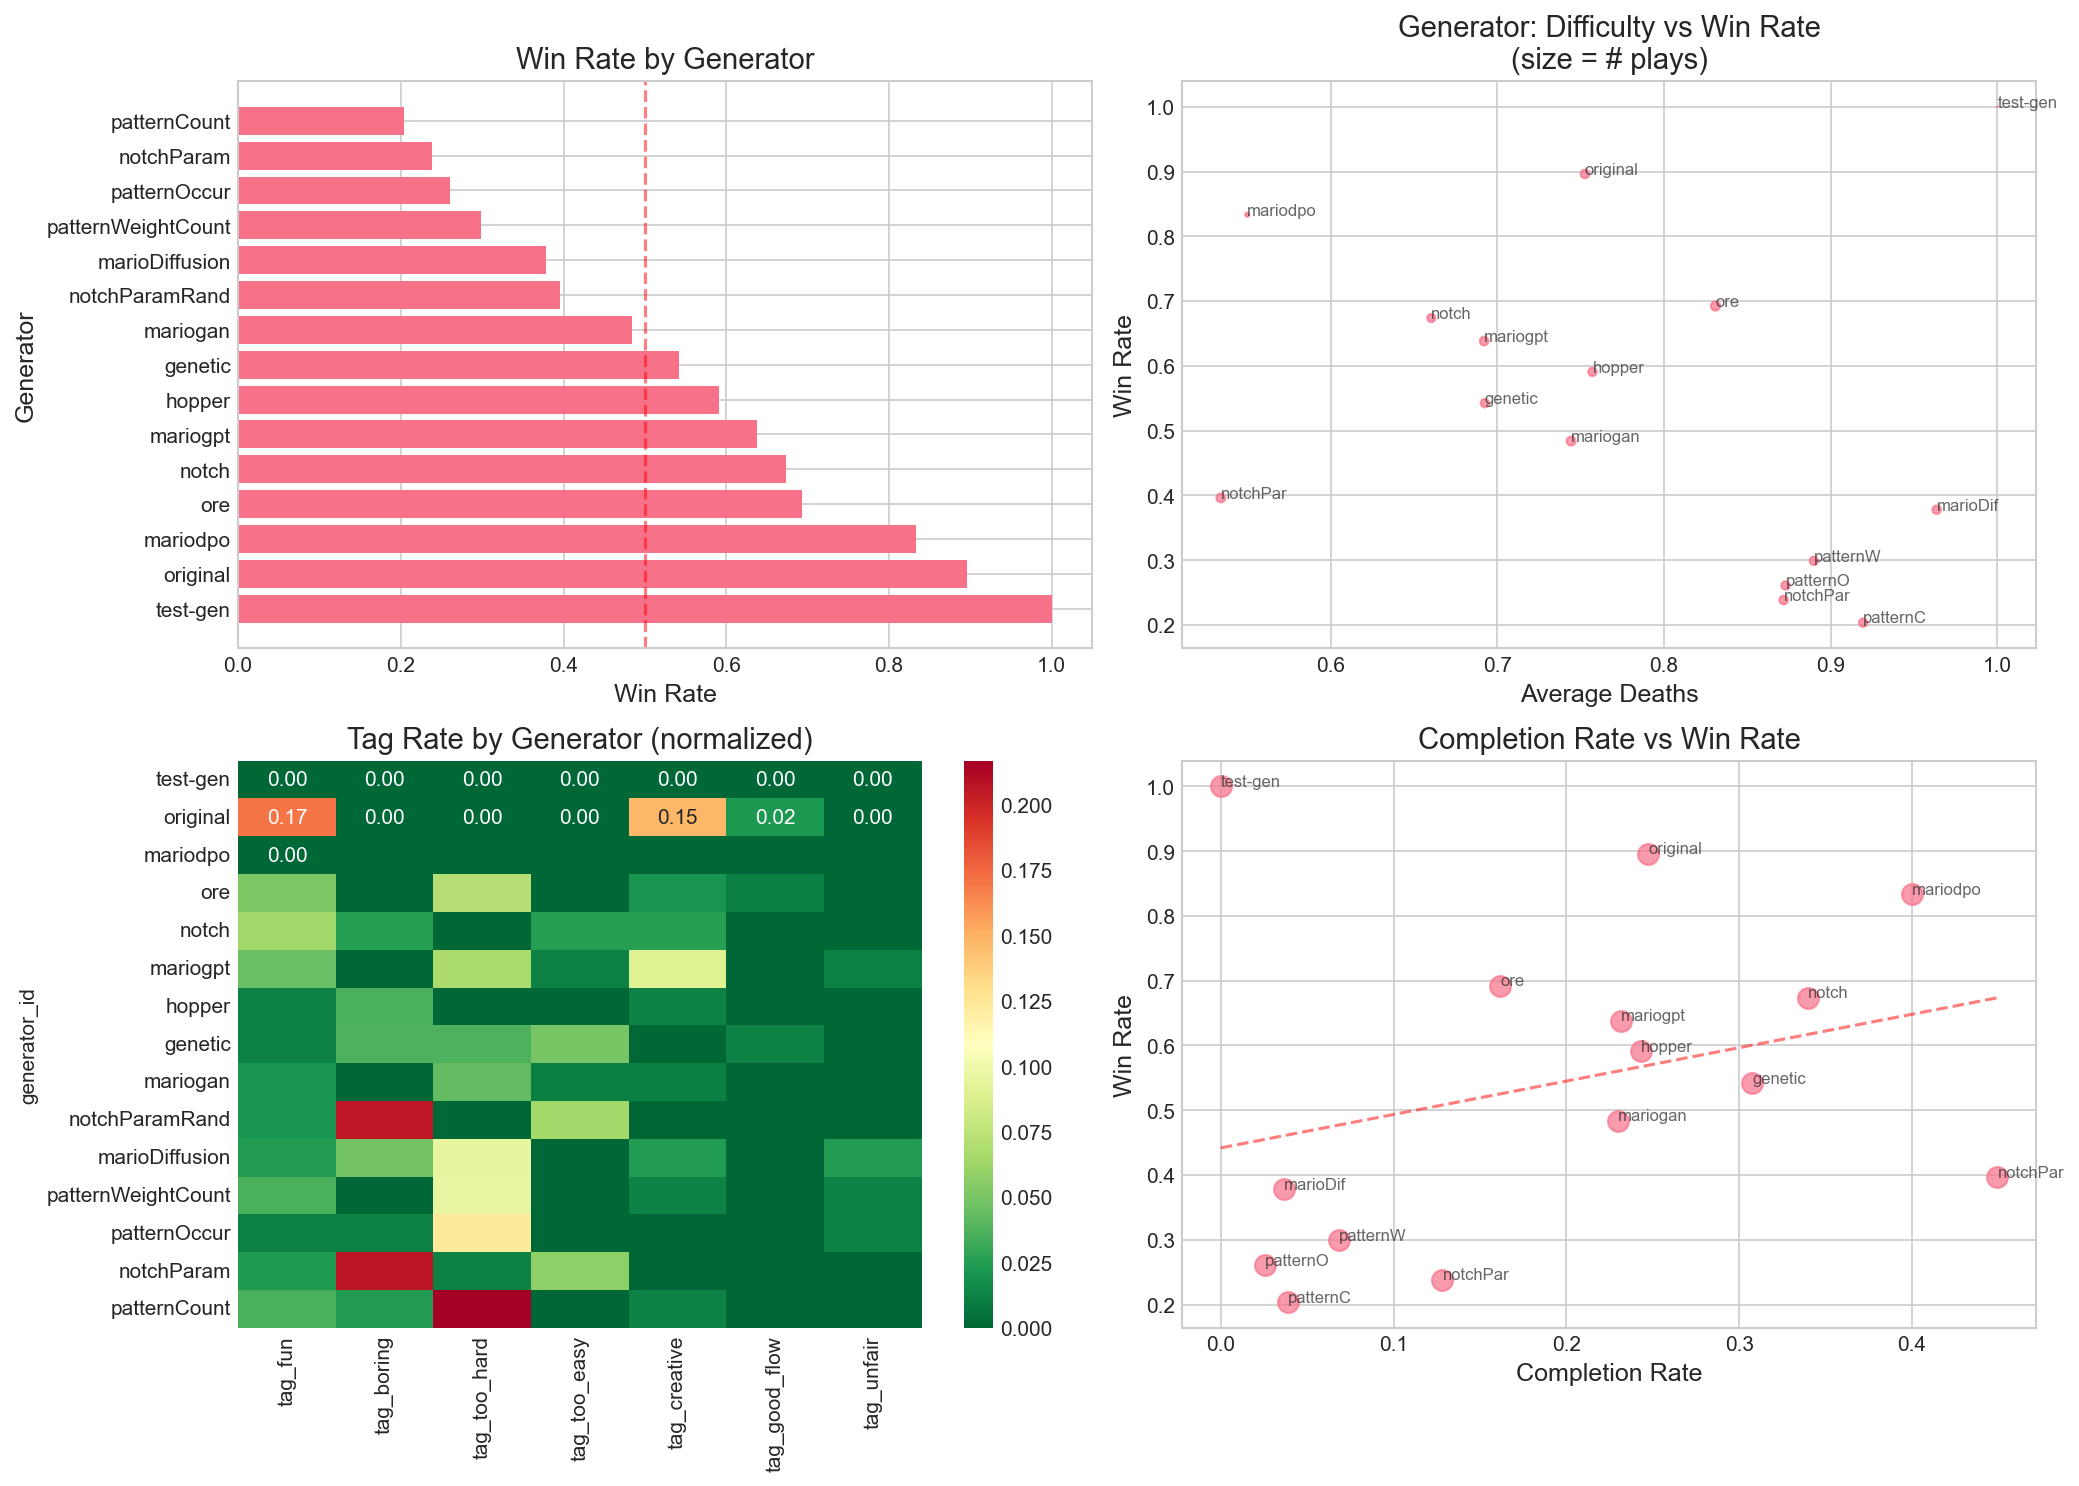
\includegraphics[width=\textwidth]{generator_comparison.png}
\caption{Generator comparison showing win rates, difficulty relationships, tag profiles, and completion rate correlations across all 14 generators.}
\label{fig:generator-comparison}
\end{figure}

Generator fingerprinting (Figure~\ref{fig:generator-fingerprints}) reveals distinct profiles: top performers balance moderate difficulty with high completion rates, while bottom performers exhibit high difficulty scores ($>$0.85) and low completion rates ($<$10\%).

\begin{figure}[H]
\centering
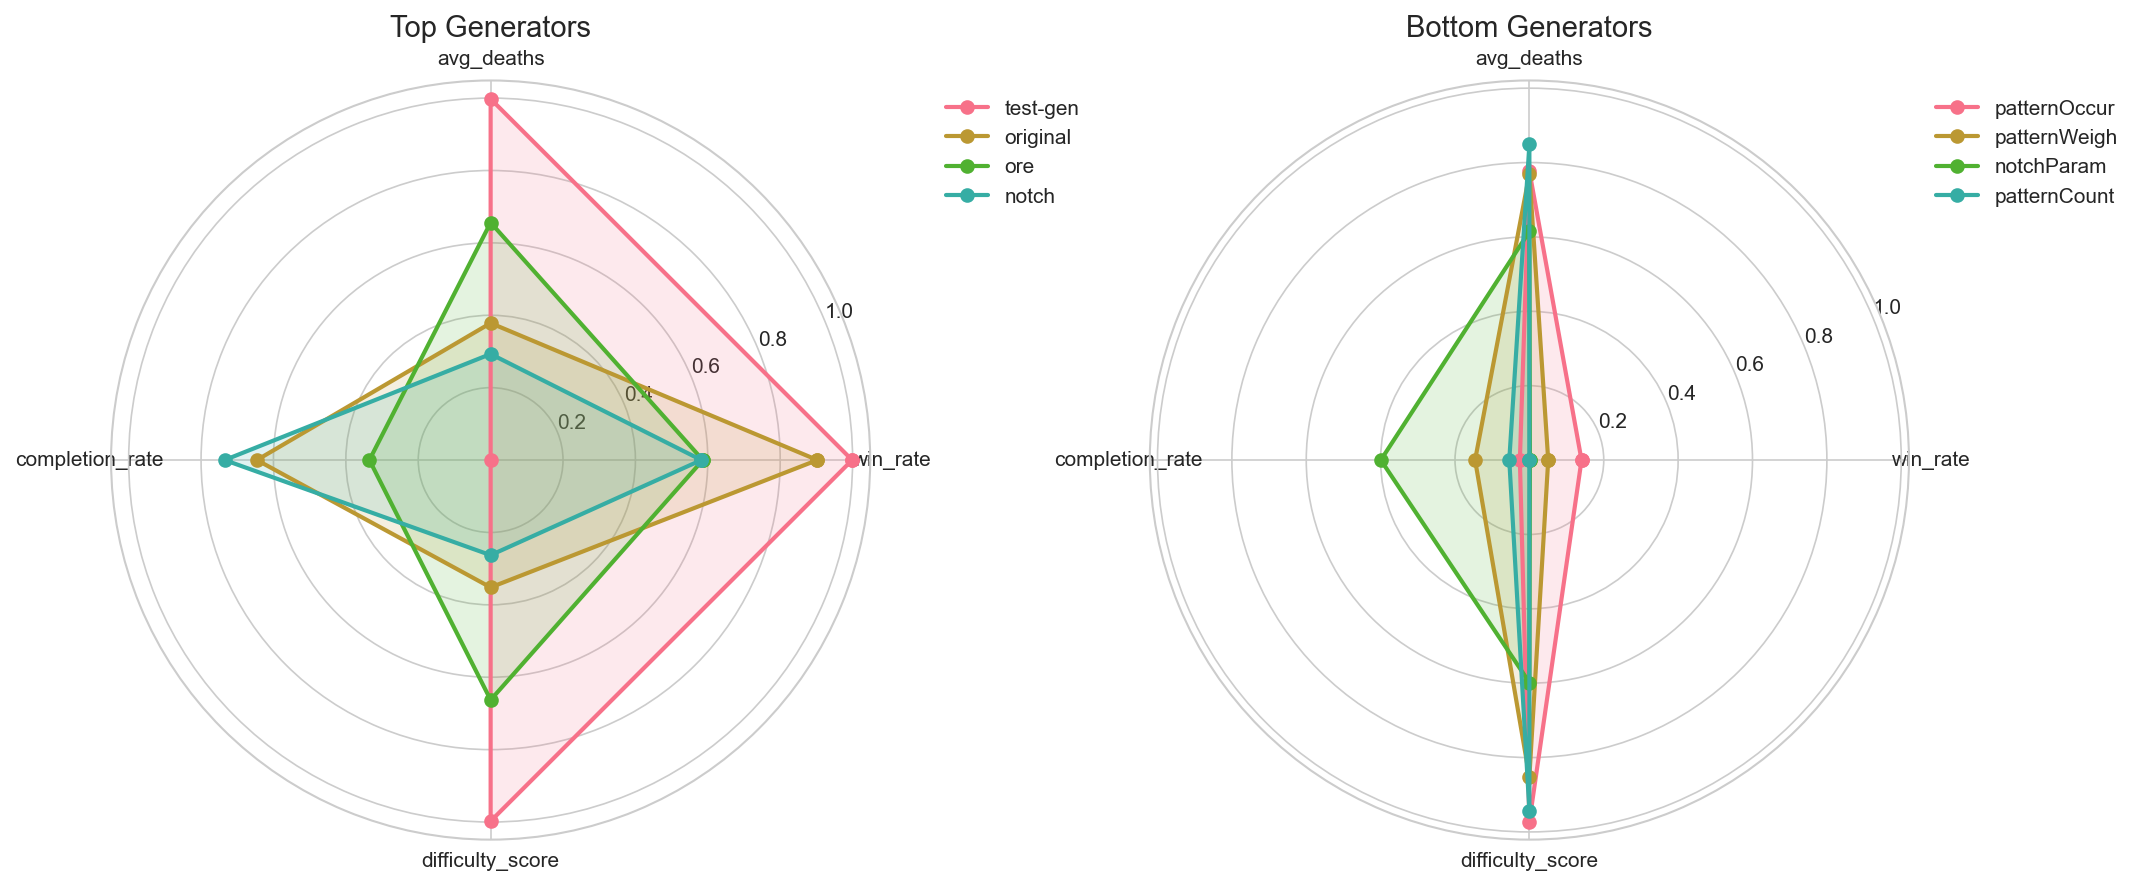
\includegraphics[width=0.9\textwidth]{generator_fingerprints.png}
\caption{Radar chart fingerprints comparing normalized metrics for top-performing (left) and bottom-performing (right) generators.}
\label{fig:generator-fingerprints}
\end{figure}

\subsection{RQ1: What Makes a Good Generator?}
\label{subsec:rq1}

We tested three hypotheses regarding level quality:

\subsubsection{H1: Optimized Difficulty (Flow Channel)}

\textbf{Hypothesis}: Levels with moderate difficulty (15-40\% death rate) have higher win rates than levels with extreme difficulty.

\textbf{Results}: Spearman correlation $r = -0.149$, $p = 0.313$. No inverted-U pattern was detected; instead, a linear relationship suggests that easier levels are simply preferred. Analysis was limited by insufficient data in higher difficulty bins.

\textbf{Conclusion}: \textbf{Not supported}. Players prefer easier levels; the ``flow channel'' theory does not hold in blind A/B comparisons.

\begin{figure}[H]
\centering
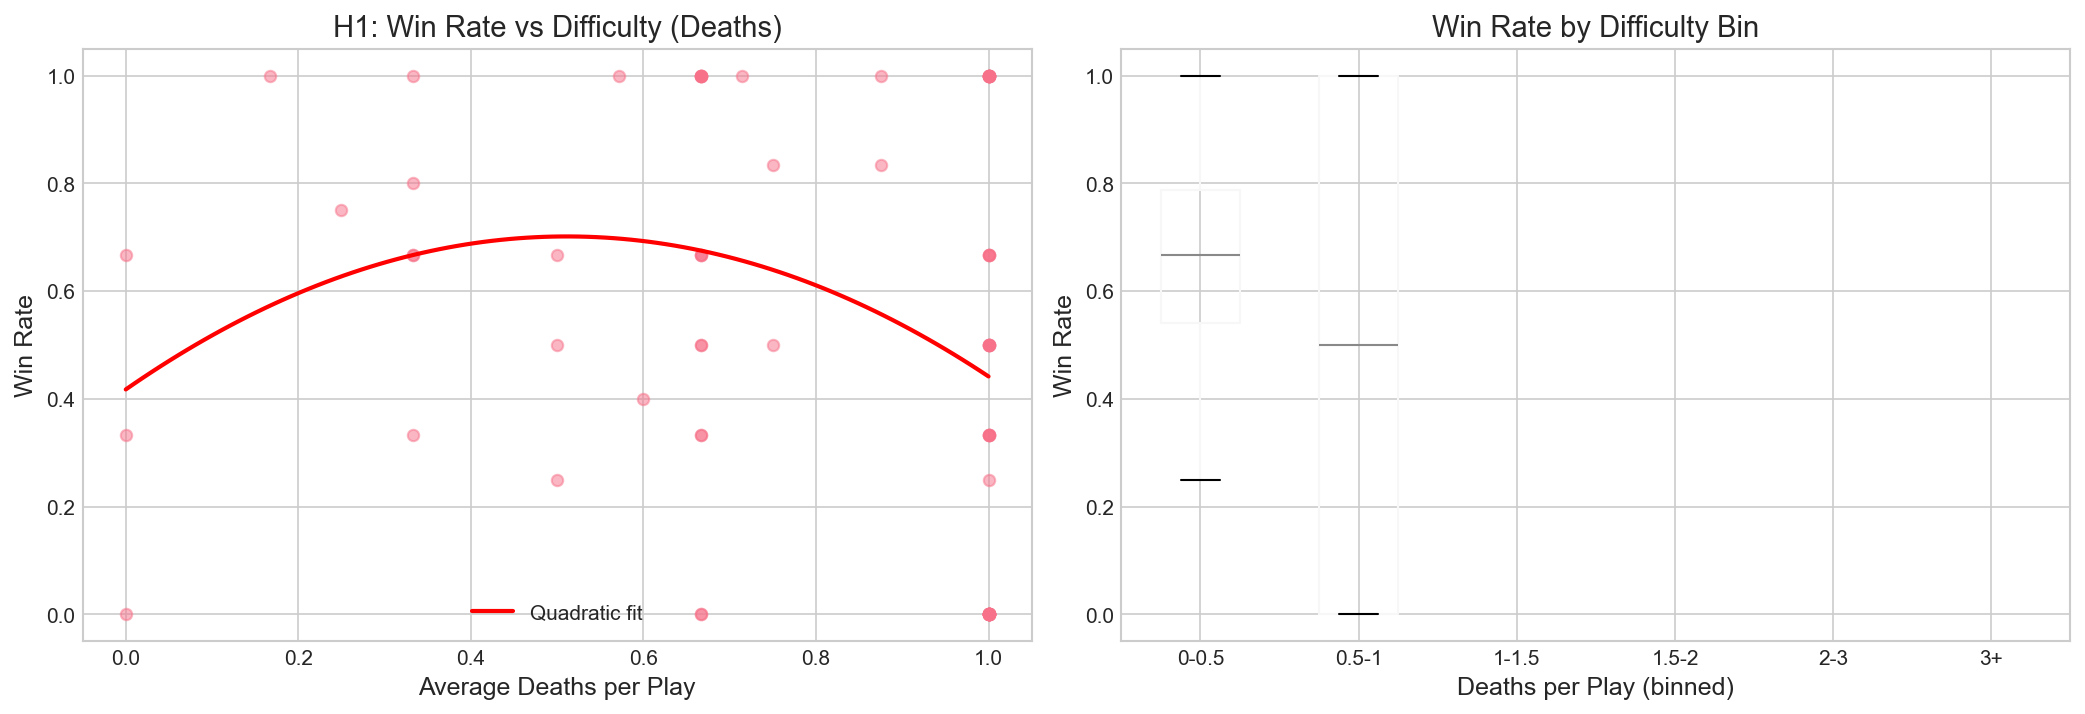
\includegraphics[width=\textwidth]{h1_difficulty_vs_winrate.png}
\caption{H1 analysis: Win rate vs. difficulty (death rate). Quadratic regression shows no inverted-U pattern; lower difficulty correlates linearly with higher win rate.}
\label{fig:h1-difficulty}
\end{figure}

\subsubsection{H2: Structural Variety}

\textbf{Hypothesis}: Levels with higher structural variety are preferred over flat or repetitive levels.

\textbf{Results}: Using tag-based proxies (structural features were null in exports):
\begin{itemize}
    \item Creative tag $\leftrightarrow$ Win rate: $r = 0.416$, $p = 0.003$ (significant)
    \item Boring tag $\leftrightarrow$ Win rate: $r = -0.246$, $p = 0.092$ (marginal)
\end{itemize}

\textbf{Conclusion}: \textbf{Partially supported}. Levels tagged as ``creative'' are significantly more likely to win comparisons.

\begin{figure}[H]
\centering
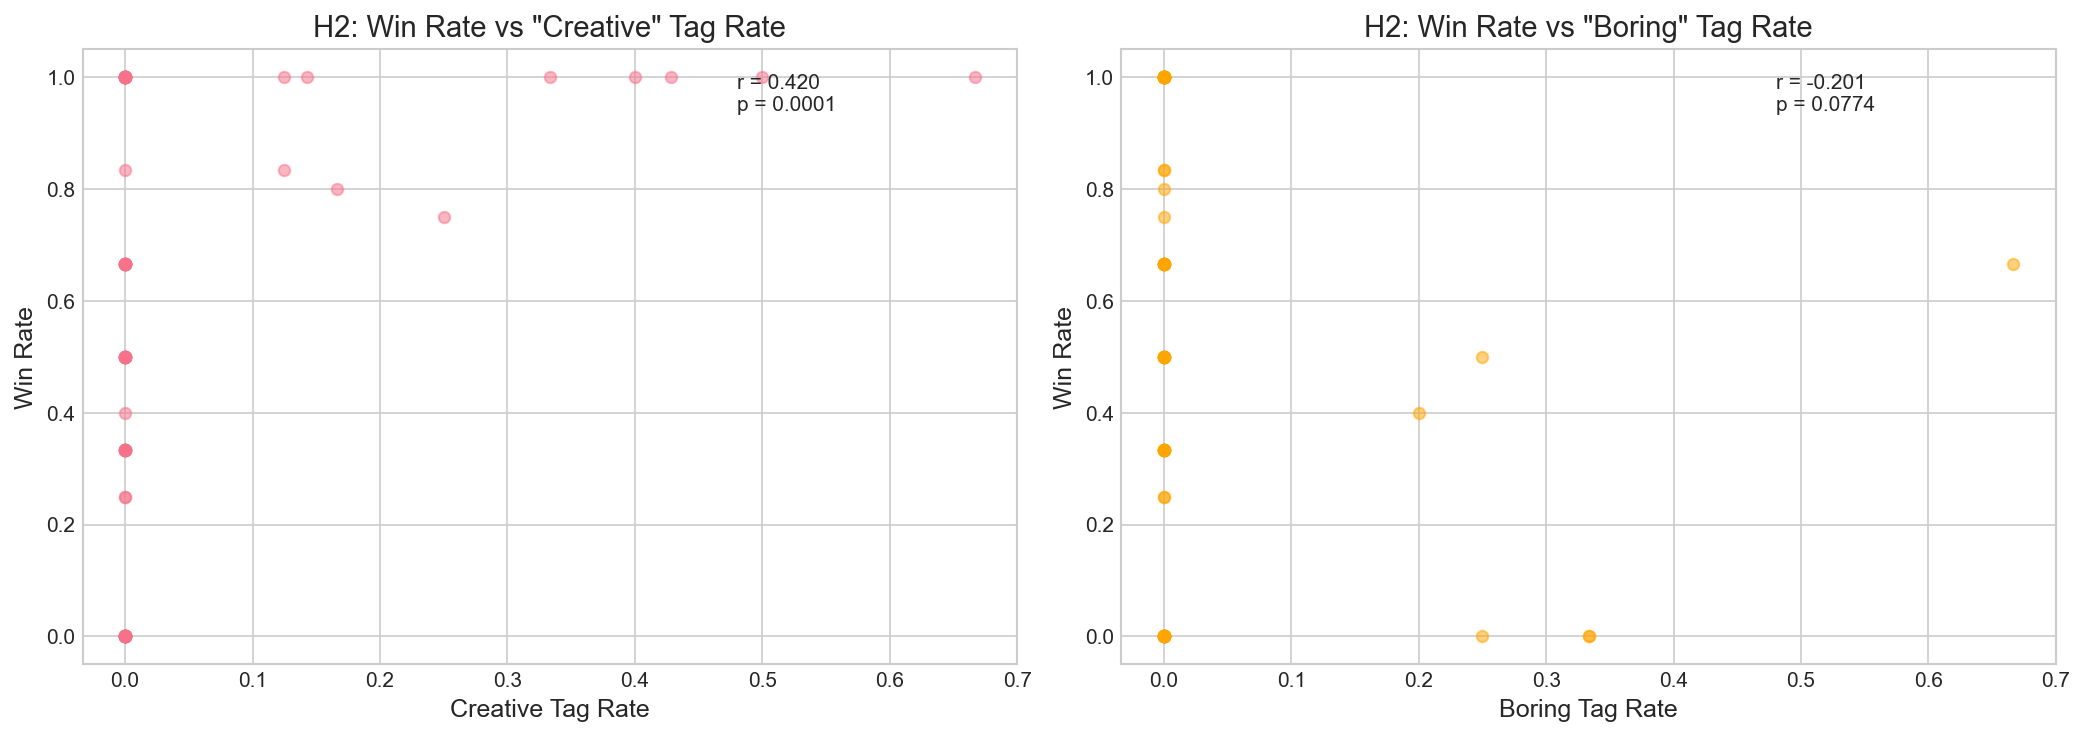
\includegraphics[width=\textwidth]{h2_structural_variety.png}
\caption{H2 analysis: Win rate correlations with ``creative'' (positive) and ``boring'' (negative) tag rates.}
\label{fig:h2-variety}
\end{figure}

\subsubsection{H3: Path Freedom (Agency)}

\textbf{Hypothesis}: Players prefer levels that allow for spatial exploration rather than strict linear paths.

\textbf{Results}: Mann-Whitney U tests comparing trajectory metrics between winning and losing levels:

\begin{table}[H]
\centering
\caption{H3: Trajectory Metrics Comparison (Won vs. Lost Levels)}
\label{tab:h3-results}
\begin{tabular}{lrrrr}
\toprule
\textbf{Metric} & \textbf{Won Mean} & \textbf{Lost Mean} & \textbf{U-stat} & \textbf{p-value} \\
\midrule
Unique Tiles Visited & 68.71 & 42.10 & 1486.5 & \textbf{0.004} \\
Backtrack Ratio & 0.13 & 0.21 & 1401.5 & \textbf{0.024} \\
Max X Reached & 1532.9 & 1094.8 & 1380.0 & \textbf{0.038} \\
Avg Speed & 34.29 & 31.85 & 1249.0 & 0.272 \\
\bottomrule
\end{tabular}
\end{table}

\textbf{Conclusion}: \textbf{Strongly supported}. Winning levels enable 63\% more spatial exploration ($p = 0.004$), have lower backtrack ratios (smoother flow), and allow greater horizontal progress.

\begin{figure}[H]
\centering
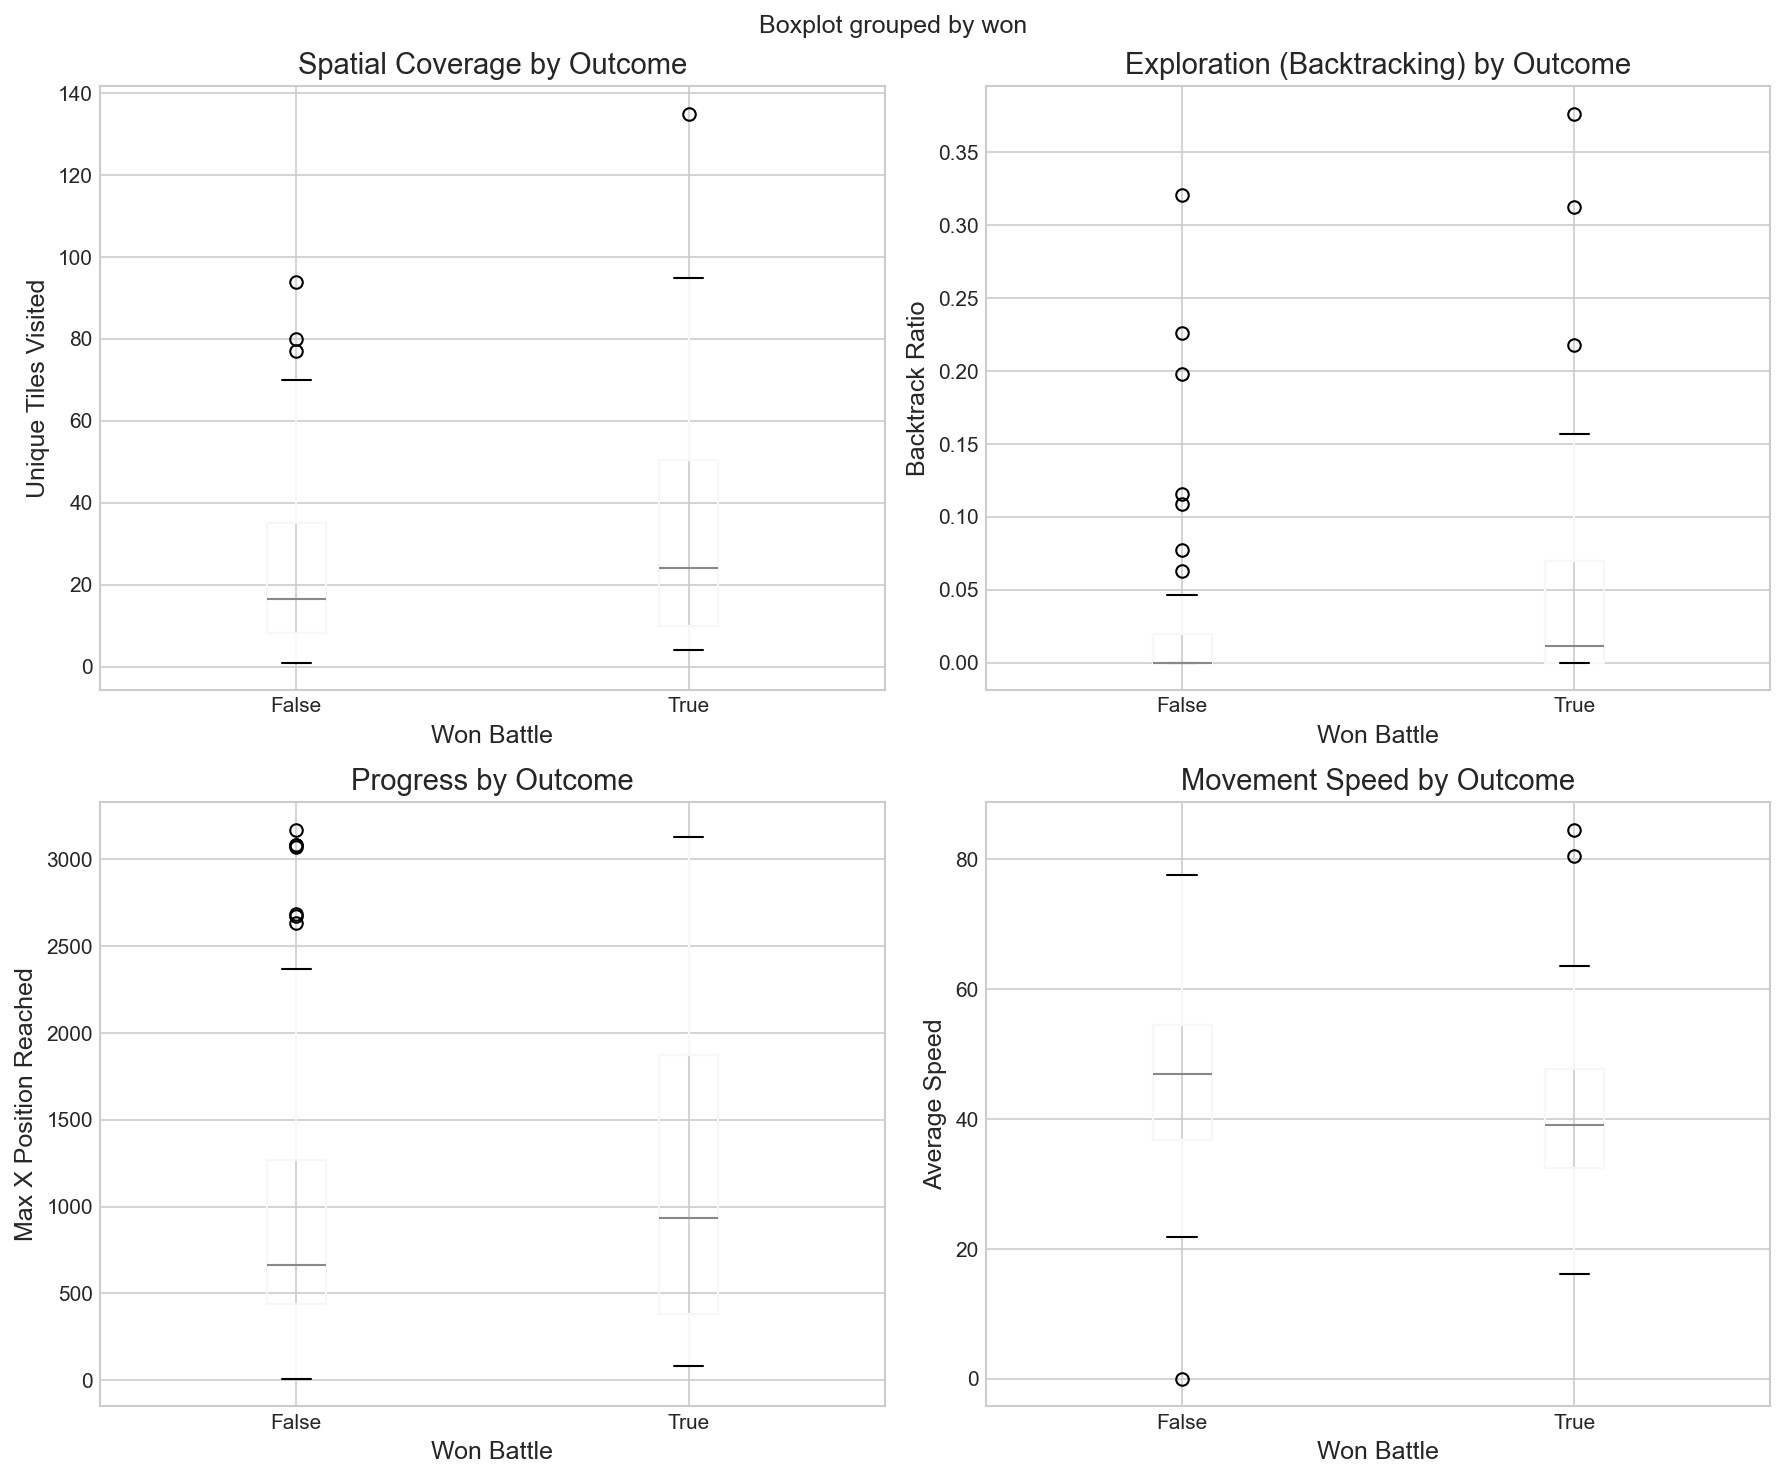
\includegraphics[width=\textwidth]{h3_path_freedom.png}
\caption{H3 analysis: Trajectory metrics comparison between won and lost levels. Winning levels show significantly higher spatial coverage and level progress.}
\label{fig:h3-agency}
\end{figure}

\subsection{RQ2: Player Preference Consistency}
\label{subsec:rq2}

\subsubsection{H4: Preference Clusters}

\textbf{Hypothesis}: Distinct player preference clusters exist based on playstyle.

\textbf{Methods}: Hierarchical clustering (Ward's method) on 12 players with $\geq$5 votes using behavioral features: avg\_deaths, avg\_duration, completion\_rate, avg\_jumps, preferred\_difficulty.

\textbf{Results}: Three clusters emerged:

\begin{table}[H]
\centering
\caption{Player Cluster Profiles}
\label{tab:clusters}
\begin{tabular}{lrrrrrrr}
\toprule
\textbf{Cluster} & \textbf{n} & \textbf{Votes} & \textbf{Deaths} & \textbf{Duration} & \textbf{Completion} & \textbf{Jumps} \\
\midrule
0 ``Explorers'' & 2 & 60 & 0.61 & 29.6s & 34.7\% & 24.1 \\
1 ``Mainstream'' & 6 & 317 & 0.83 & 15.2s & 15.7\% & 11.0 \\
2 ``Strugglers'' & 4 & 39 & 0.94 & 11.8s & 2.5\% & 5.8 \\
\bottomrule
\end{tabular}
\end{table}

\textbf{Conclusion}: \textbf{Supported}. Clear behavioral profiles emerge: ``Explorers'' (thorough, high completion), ``Mainstream'' (balanced, most active), and ``Strugglers'' (low completion, high deaths).

\begin{figure}[H]
\centering
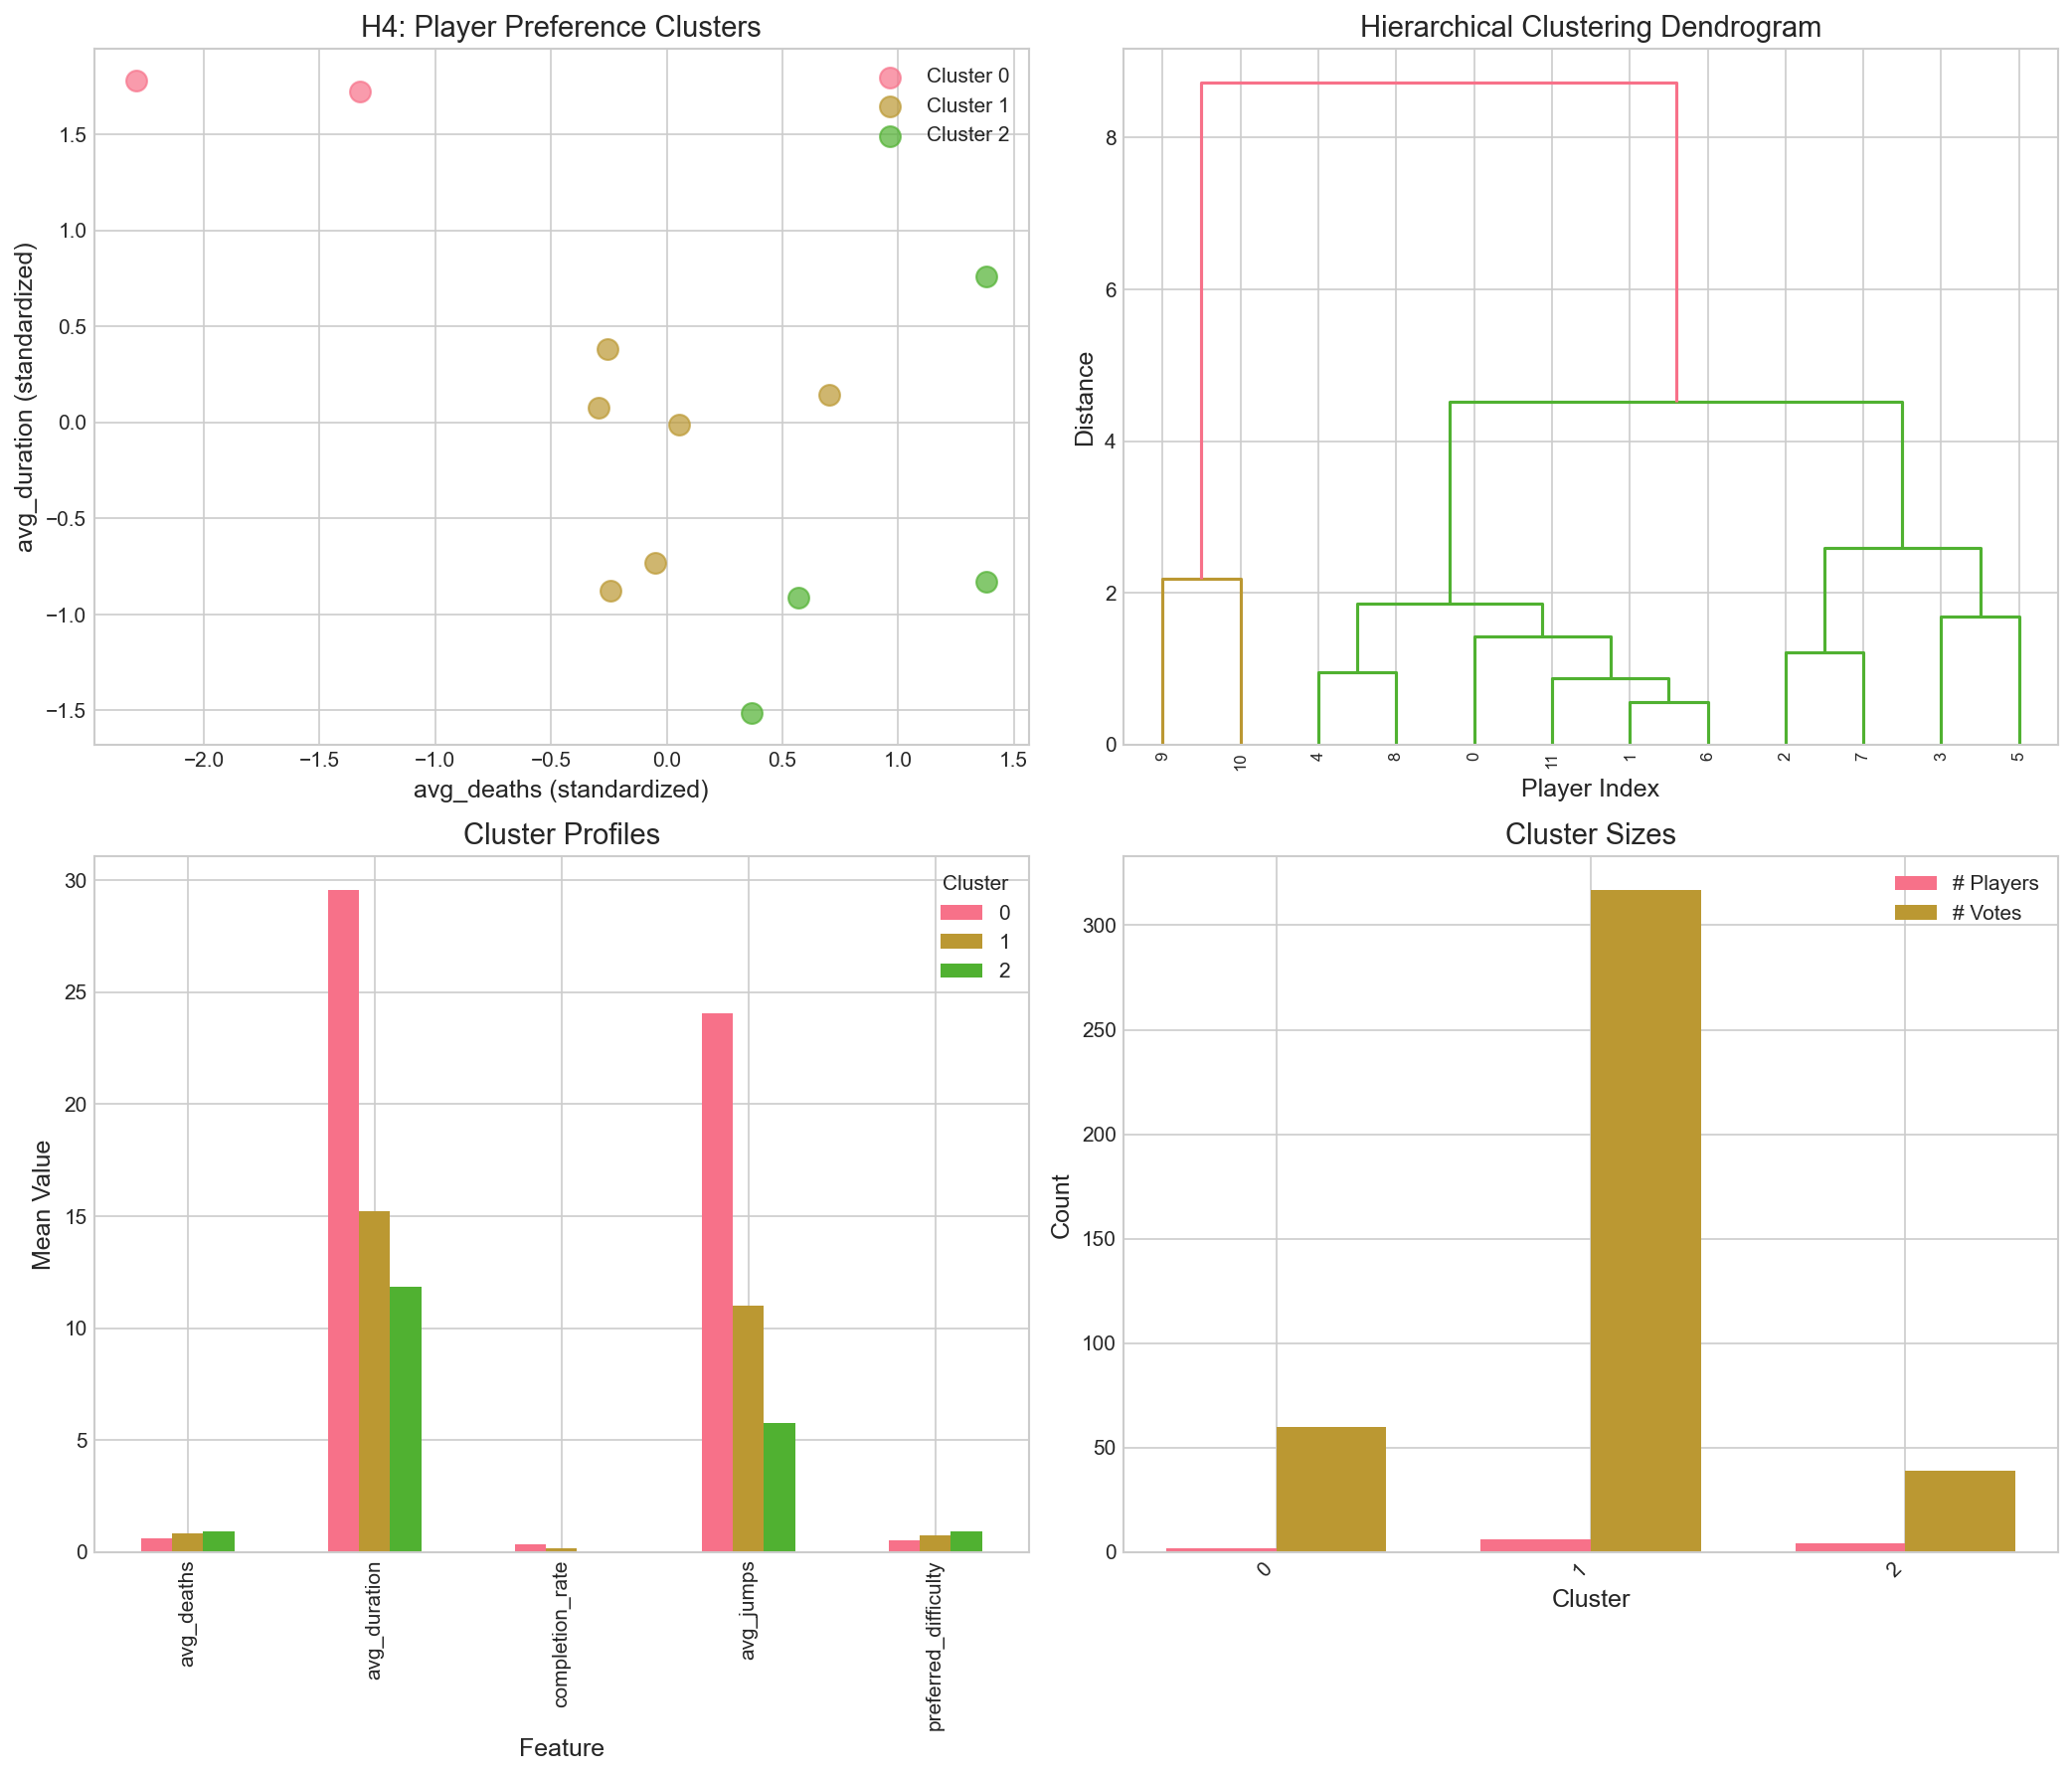
\includegraphics[width=\textwidth]{h4_preference_clusters.png}
\caption{H4 analysis: Player preference clusters. Left: 2D projection of clusters; Right: Dendrogram showing hierarchical structure; Bottom: Cluster profiles and sizes.}
\label{fig:h4-clusters}
\end{figure}

\subsubsection{H5: Skill-Consistency Relationship}

\textbf{Hypothesis}: Higher-skill players show more consistent preferences.

\textbf{Results}: 
\begin{itemize}
    \item ANOVA (CV across skill quartiles): $F = 0.172$, $p = 0.912$
    \item Spearman correlation (skill vs. consistency): $r = 0.176$, $p = 0.584$
\end{itemize}

\textbf{Conclusion}: \textbf{Not supported}. Consistency is uniform across skill levels; skill cannot be used as a proxy for preference reliability.

\begin{figure}[H]
\centering
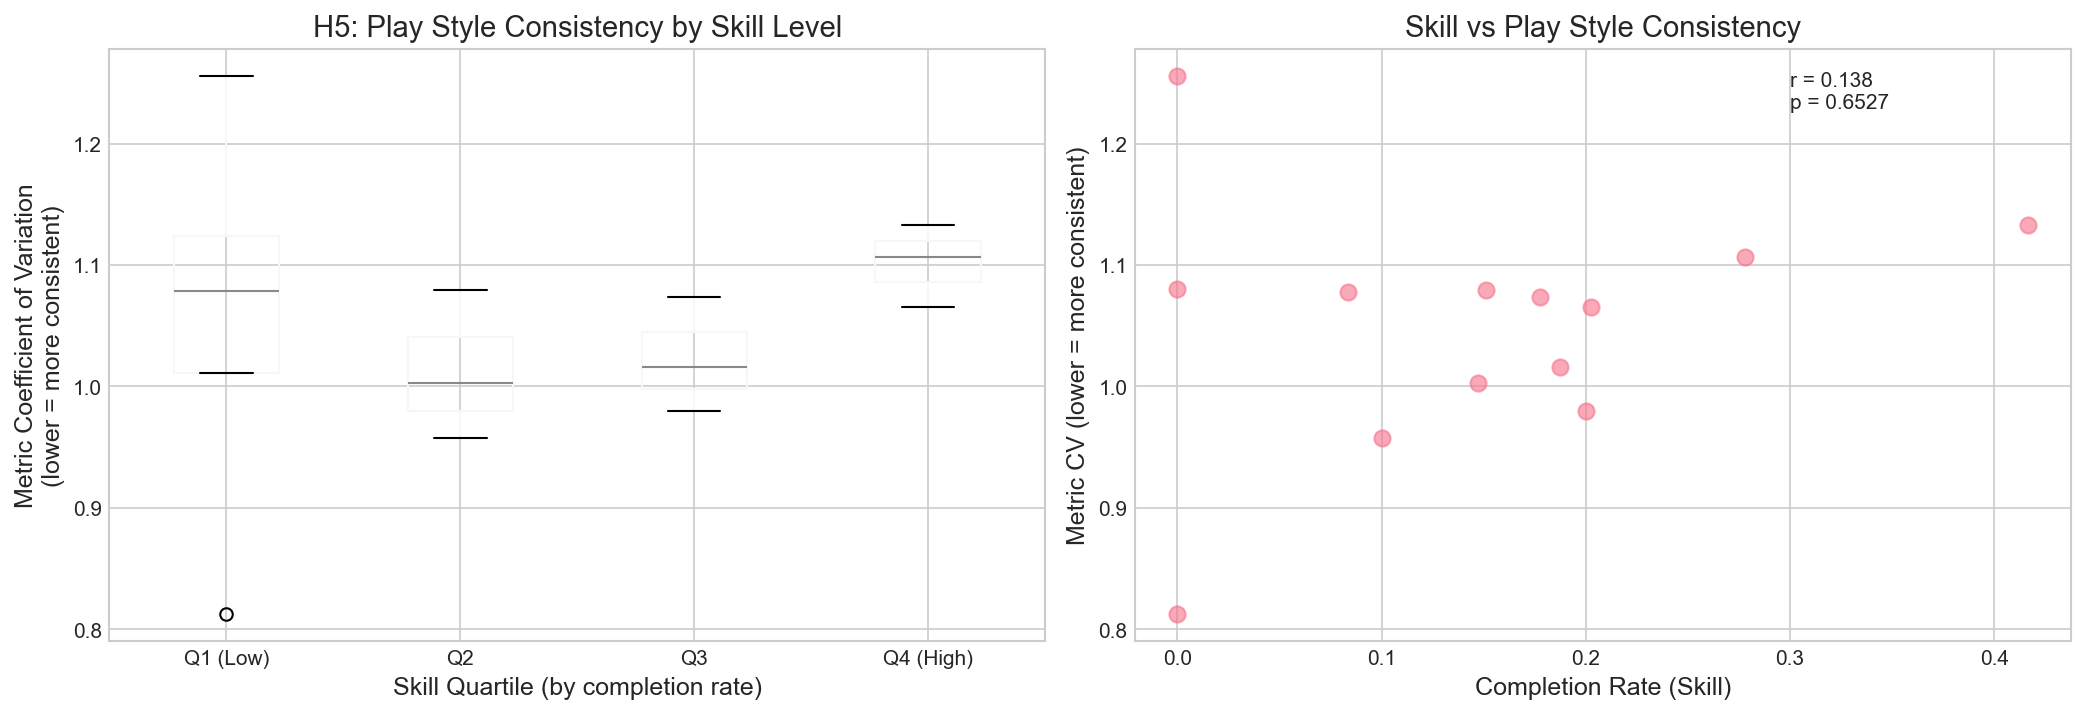
\includegraphics[width=\textwidth]{h5_skill_consistency.png}
\caption{H5 analysis: No relationship between player skill (completion rate) and preference consistency (coefficient of variation).}
\label{fig:h5-consistency}
\end{figure}

\subsection{RQ3: Tag Semantics}
\label{subsec:rq3}

\subsubsection{H6: Tag-Telemetry Correspondence}

\textbf{Hypothesis}: Player-assigned tags correspond to measurable gameplay differences.

\textbf{Results}: Testing tag presence against expected telemetry metrics:

\begin{table}[H]
\centering
\caption{H6: Tag Validation Against Telemetry}
\label{tab:h6-results}
\begin{tabular}{llrrrrl}
\toprule
\textbf{Tag} & \textbf{Metric} & \textbf{Has Tag} & \textbf{No Tag} & \textbf{U-stat} & \textbf{p-value} & \textbf{Matches} \\
\midrule
tag\_too\_hard & avg\_deaths & 0.867 & 0.781 & 121.0 & 0.634 & $\checkmark$ \\
tag\_fun & completion\_rate & 0.339 & 0.167 & 292.5 & \textbf{0.049} & $\checkmark$ \\
\bottomrule
\end{tabular}
\end{table}

\textbf{Conclusion}: \textbf{Partially supported}. ``Fun'' tag significantly correlates with higher completion rate ($p = 0.049$, Cohen's $d = 0.63$).

\begin{figure}[H]
\centering
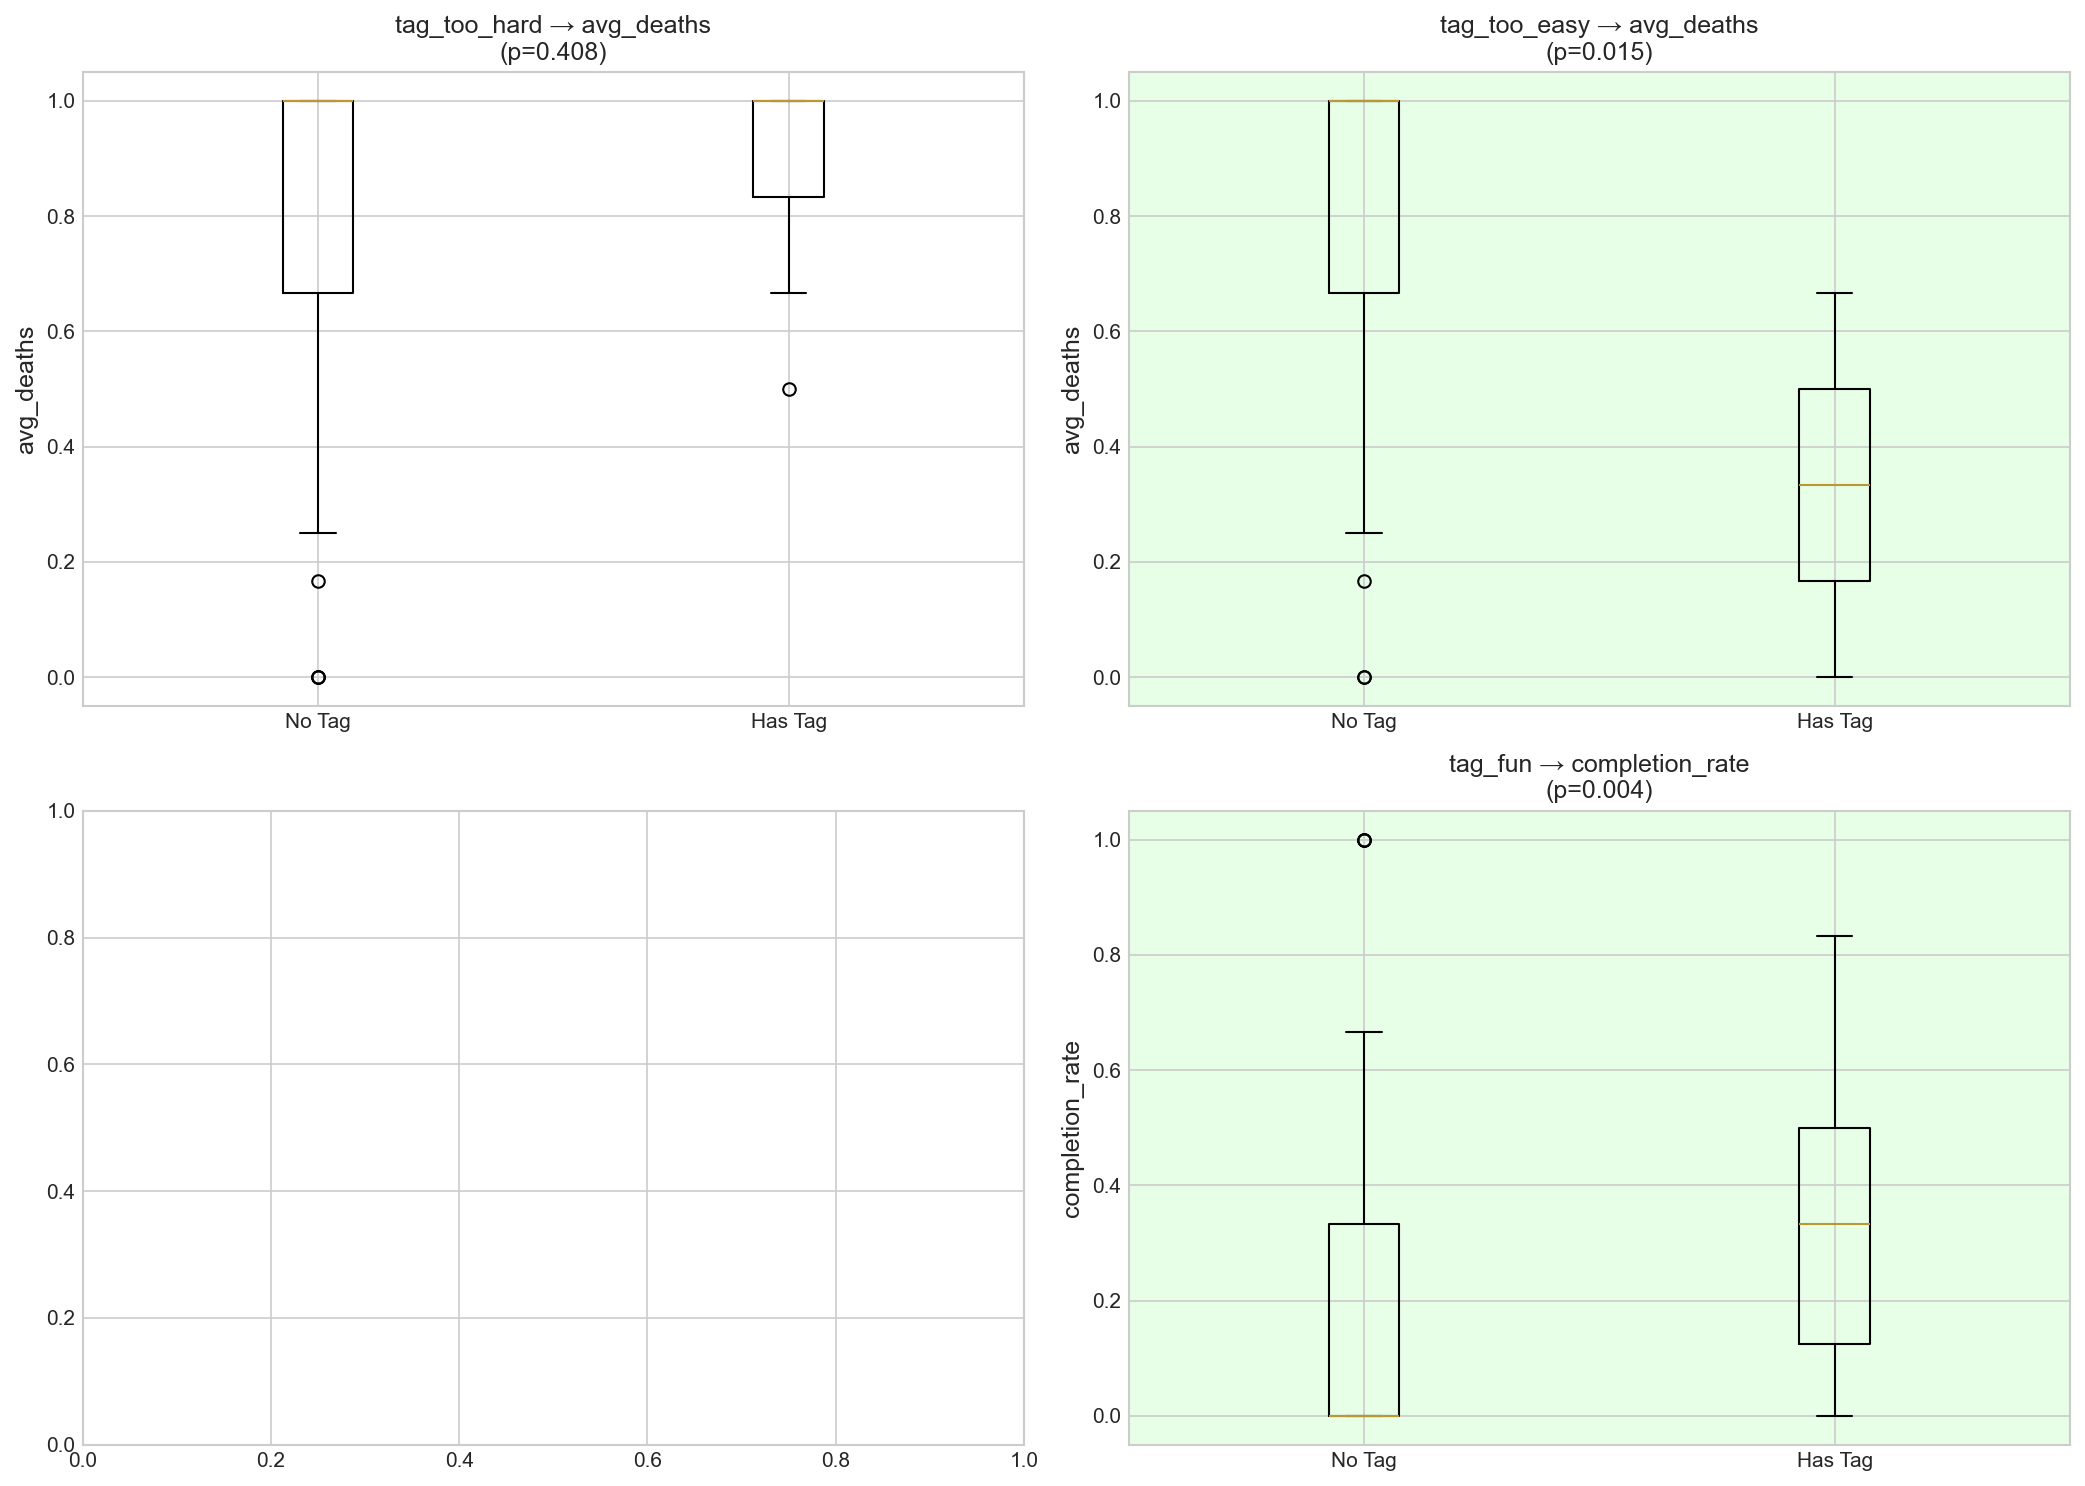
\includegraphics[width=\textwidth]{h6_tag_telemetry.png}
\caption{H6 analysis: Tag-telemetry correspondence. ``Fun'' levels show significantly higher completion rates; ``too hard'' shows expected direction but lacks significance.}
\label{fig:h6-tags}
\end{figure}

\subsubsection{H7: Feature Importance for Tags}

\textbf{Hypothesis}: Telemetry features can predict tag assignment.

\textbf{Results}: Point-biserial correlations between tag presence and features:

\begin{table}[H]
\centering
\caption{H7: Tag-Feature Correlations}
\label{tab:h7-results}
\begin{tabular}{llrr}
\toprule
\textbf{Tag} & \textbf{Feature} & \textbf{Correlation} & \textbf{p-value} \\
\midrule
tag\_too\_easy & completion\_rate & +0.353 & \textbf{0.014} \\
tag\_too\_easy & avg\_deaths & $-$0.353 & \textbf{0.014} \\
tag\_fun & avg\_deaths & $-$0.277 & 0.056 \\
tag\_fun & completion\_rate & +0.277 & 0.056 \\
tag\_creative & completion\_rate & +0.275 & 0.058 \\
\bottomrule
\end{tabular}
\end{table}

\textbf{Conclusion}: \textbf{Supported}. ``Too easy'' is well-defined by telemetry ($r = 0.35$); ``fun'' and ``creative'' show consistent patterns (higher completion, lower deaths).

\begin{figure}[H]
\centering
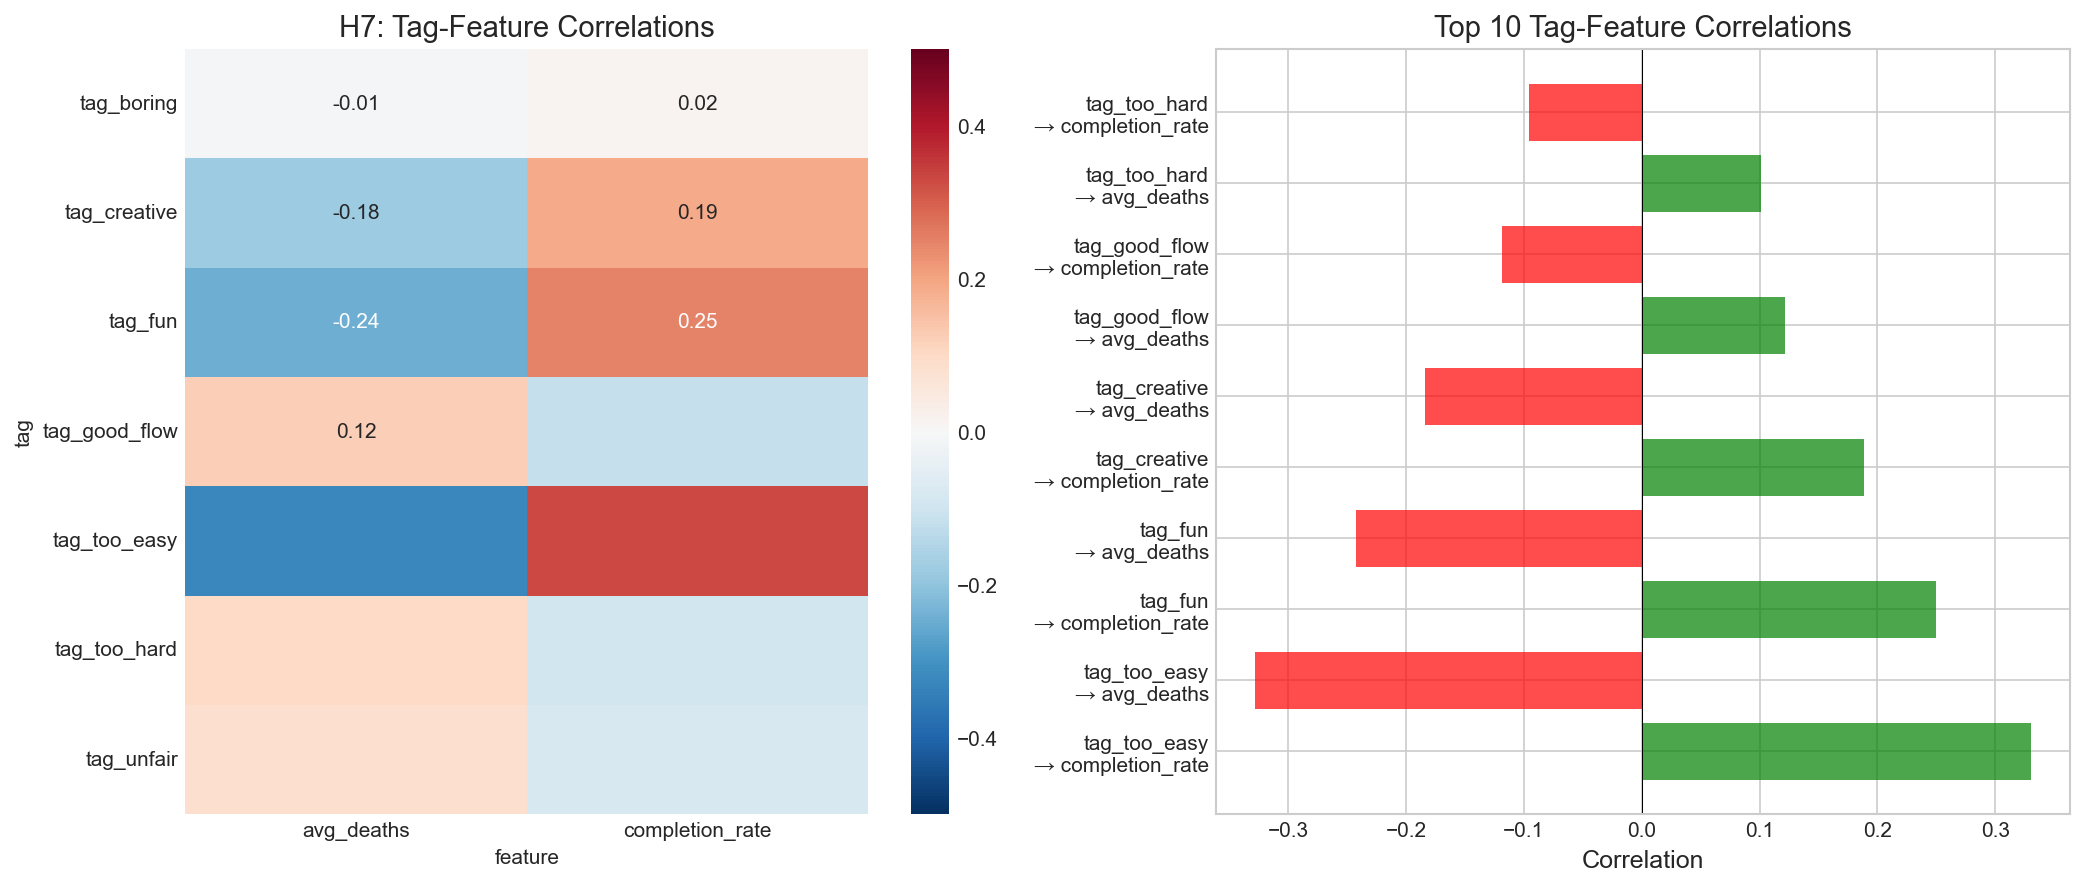
\includegraphics[width=\textwidth]{h7_tag_feature_importance.png}
\caption{H7 analysis: Tag-feature correlation heatmap (left) and top correlations (right). Completion rate and death rate are primary predictors.}
\label{fig:h7-importance}
\end{figure}

\subsubsection{Tag Distribution and Co-occurrence}

\begin{figure}[H]
\centering
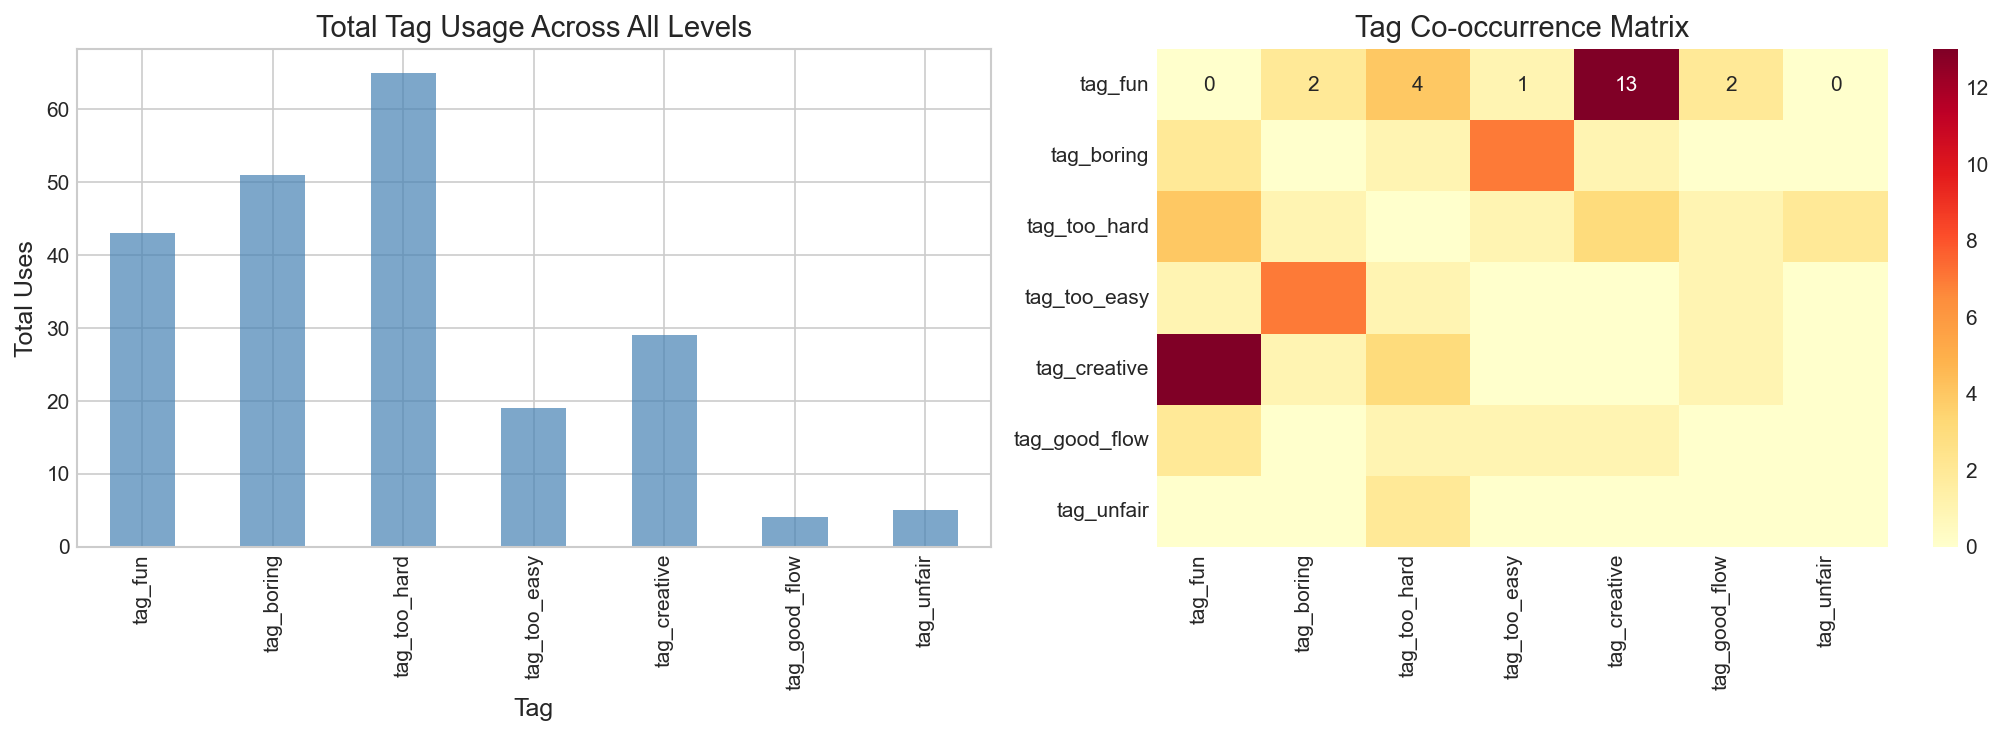
\includegraphics[width=\textwidth]{tag_distribution.png}
\caption{Tag usage distribution (left) and co-occurrence matrix (right). ``Too hard'' is most common; ``fun'' and ``creative'' strongly co-occur ($\phi = 0.419$).}
\label{fig:tag-distribution}
\end{figure}

\begin{figure}[H]
\centering
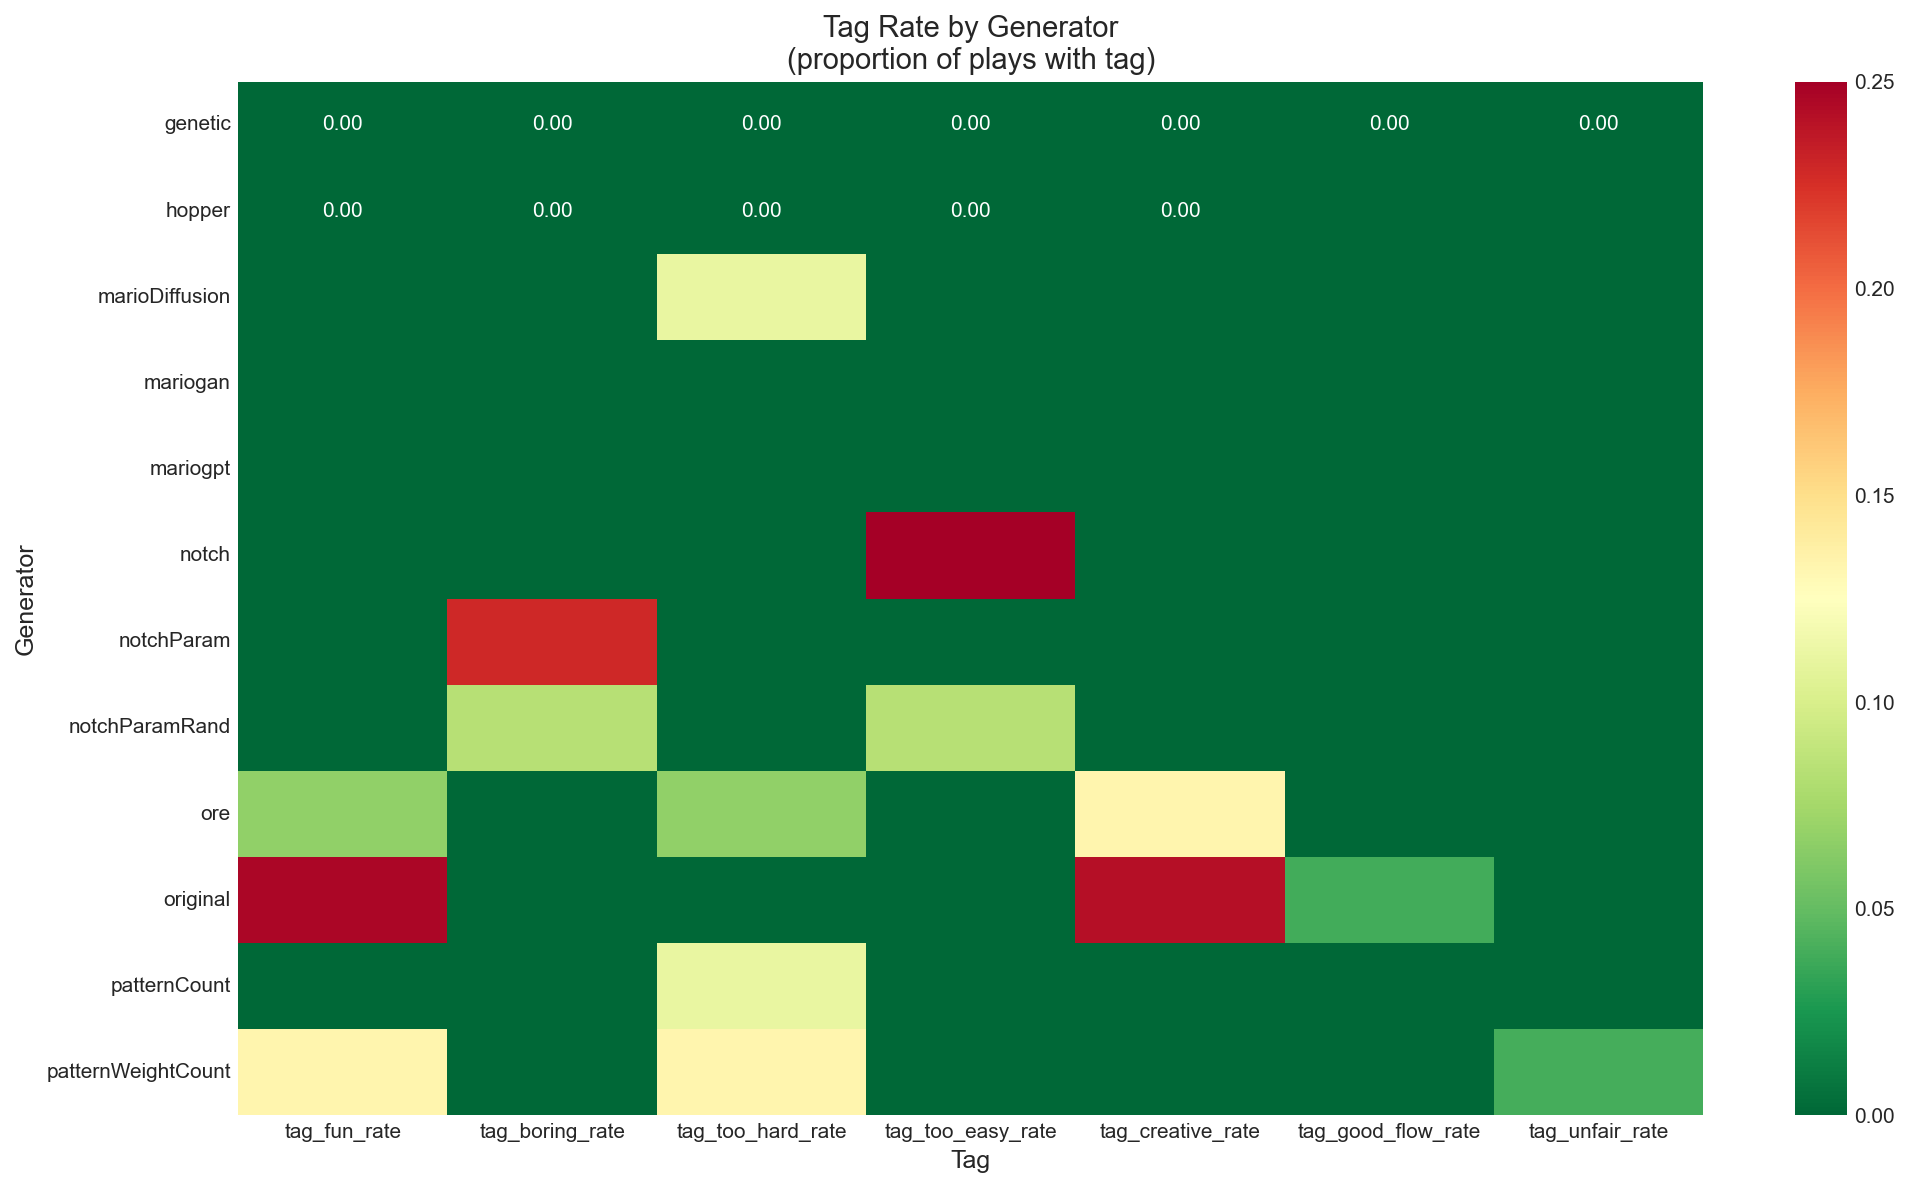
\includegraphics[width=\textwidth]{tag_by_generator.png}
\caption{Tag rate heatmap by generator. ``Original'' leads in fun (25\%) and creative (24\%); ``notchParam'' is most boring (23\%); pattern-based generators are most difficult.}
\label{fig:tag-by-generator}
\end{figure}

\subsection{Trajectory Analysis}
\label{subsec:trajectories}

Analysis of 100 player trajectories reveals movement patterns that correlate with level preference:

\begin{figure}[H]
\centering
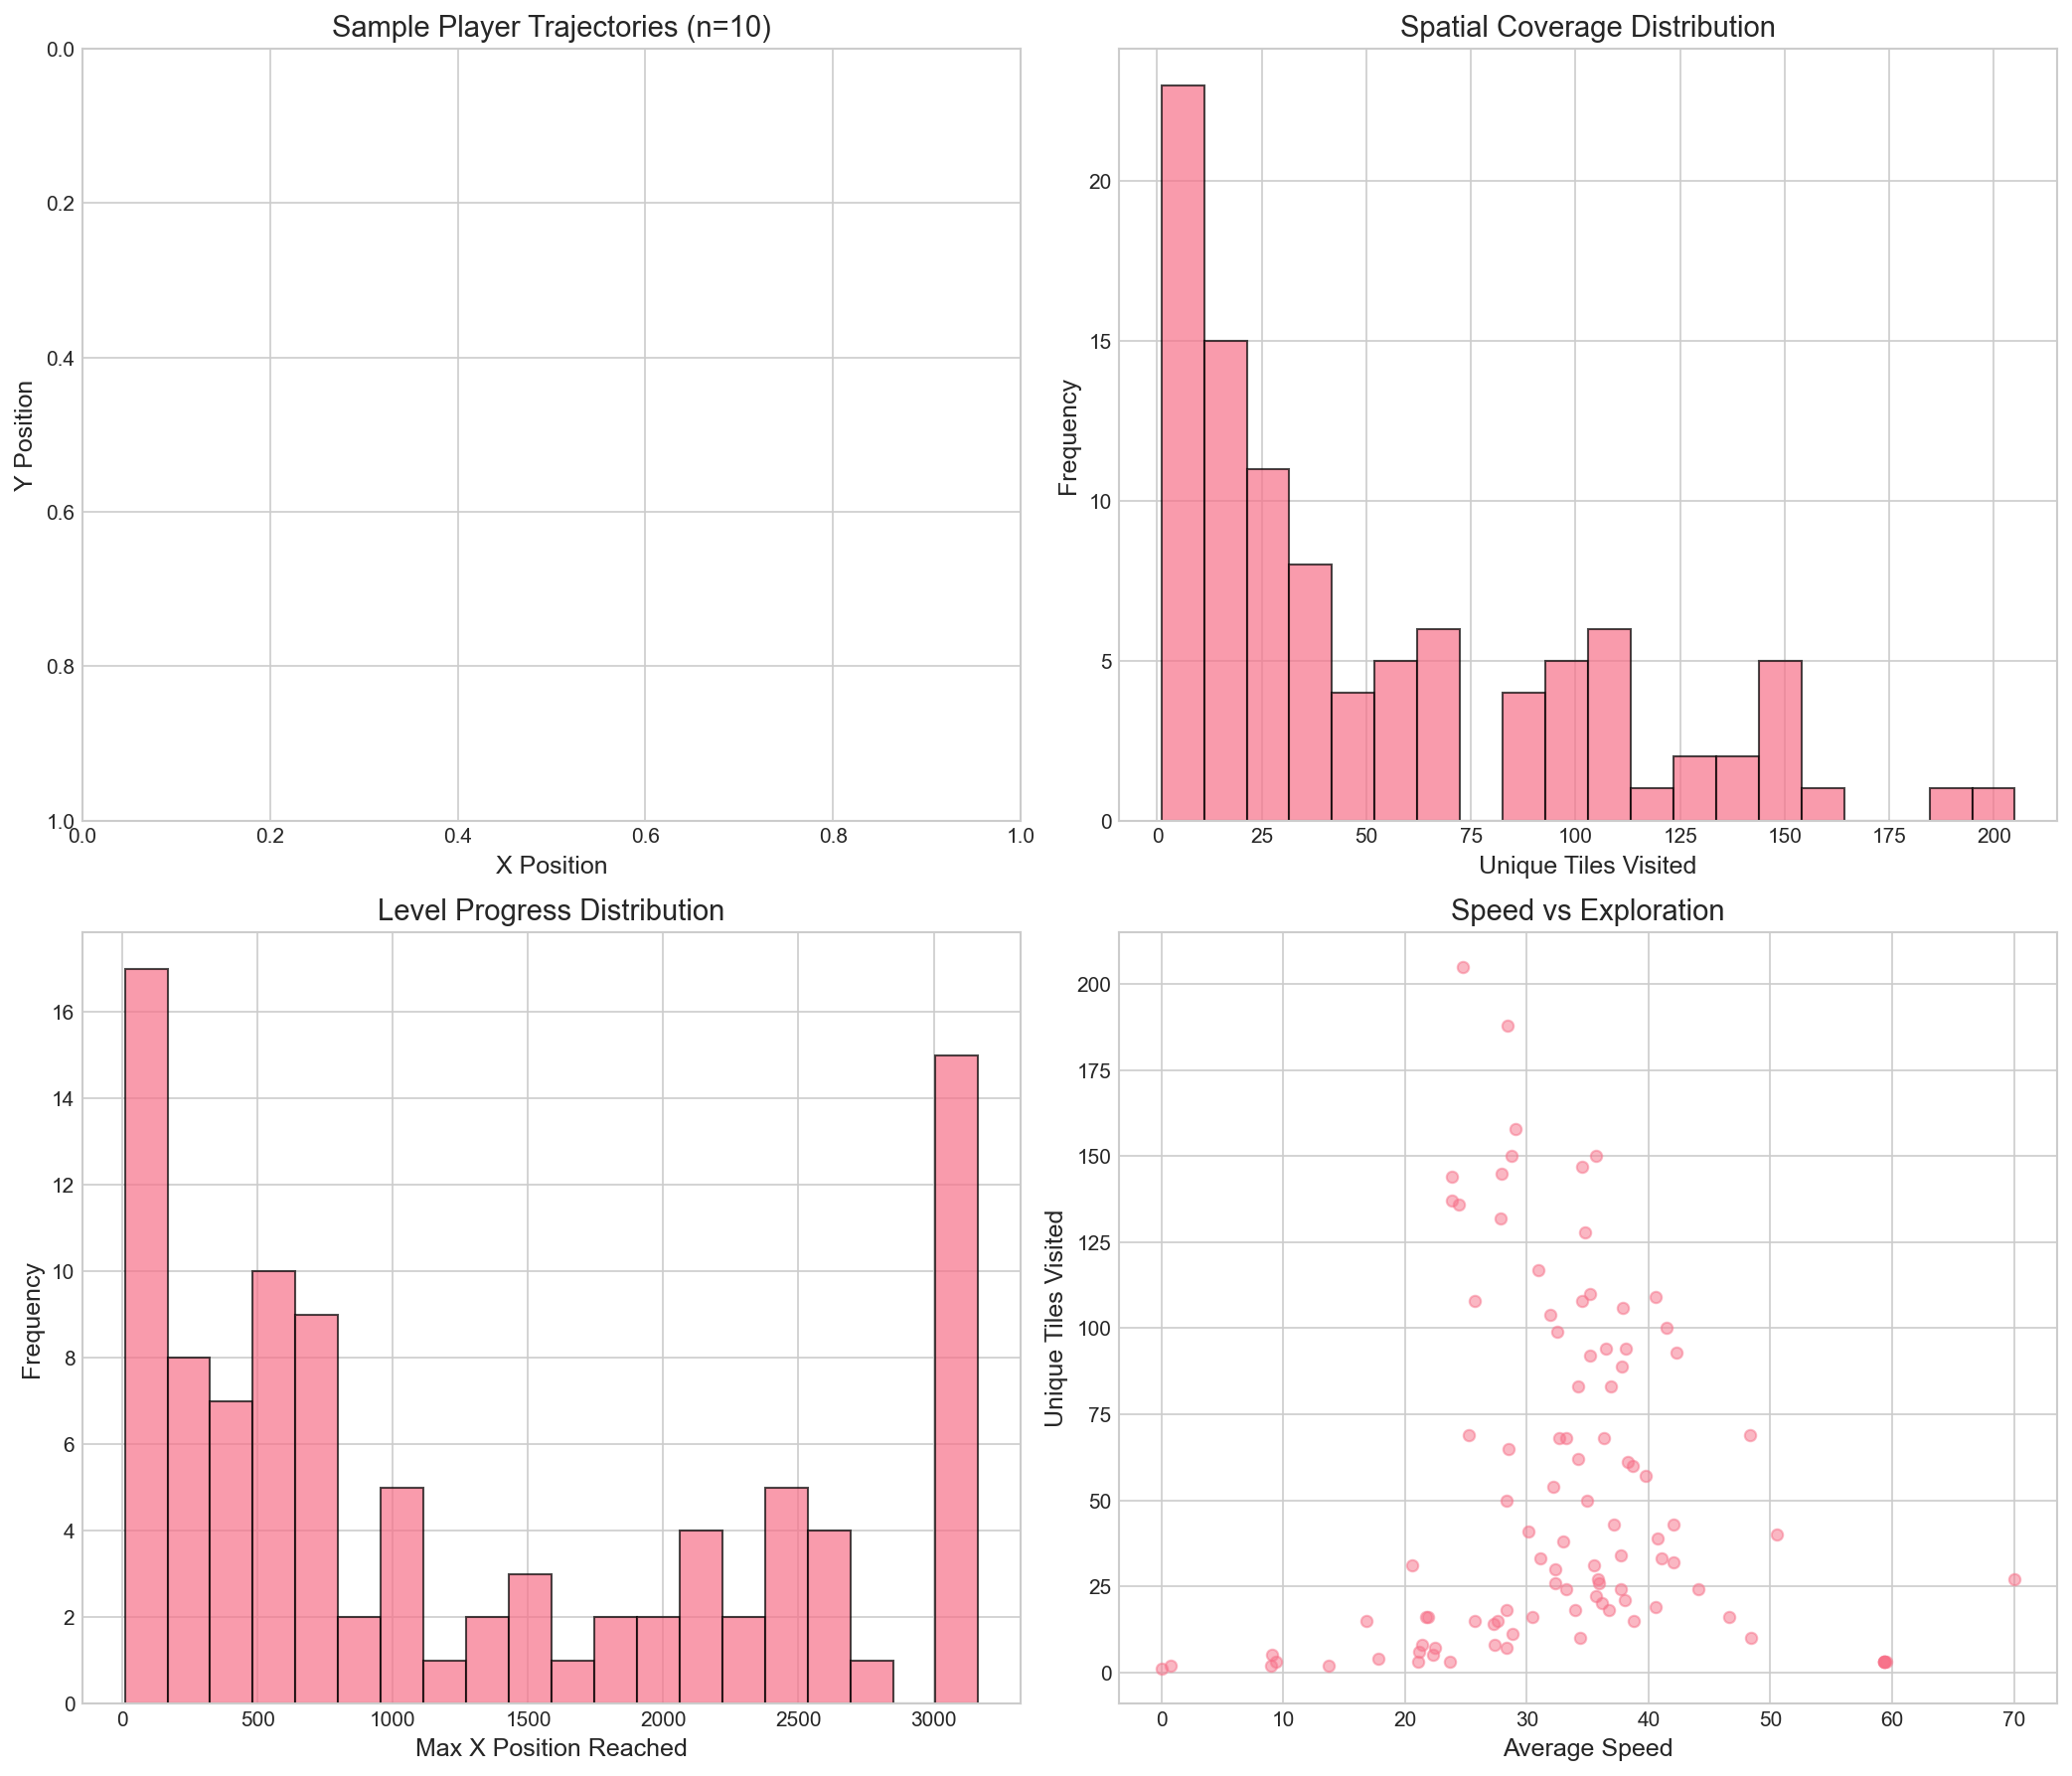
\includegraphics[width=\textwidth]{trajectory_visualization.png}
\caption{Trajectory analysis: sample paths (top-left), spatial coverage distribution (top-right), level progress distribution (bottom-left), and speed vs. exploration scatter (bottom-right).}
\label{fig:trajectories}
\end{figure}

Key trajectory statistics: average unique tiles visited = 52.4, average max X reached = 1267.2 ($\approx$60-70\% level progress), average speed = 32.93 units/second.

\subsection{Correlation Structure}
\label{subsec:correlations}

\begin{figure}[H]
\centering
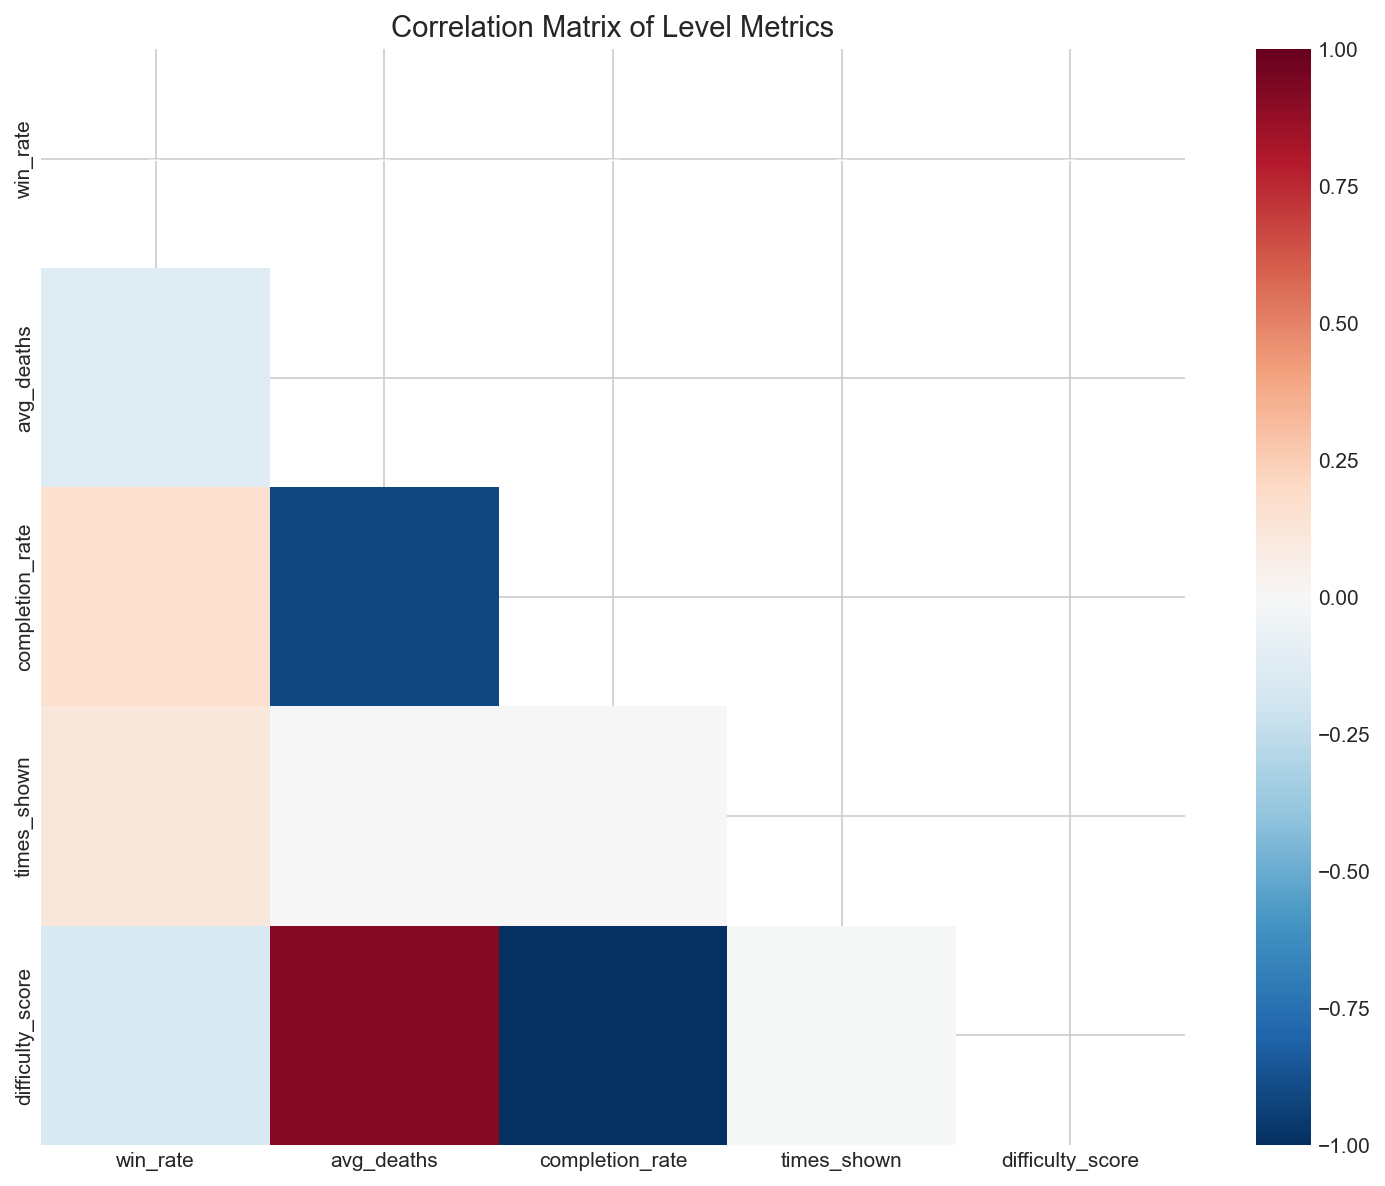
\includegraphics[width=0.7\textwidth]{correlation_matrix.png}
\caption{Correlation matrix of level metrics. Strong inverse correlation between deaths and completion ($r = -0.913$); difficulty score is derived from completion rate ($r = -1.0$).}
\label{fig:correlations}
\end{figure}

\subsection{Extended Feature Analysis}
\label{subsec:extended-features}

Three additional experiments were conducted to further identify key gameplay features influencing player preference.

\subsubsection{H8: Enemy Density and Hazard Difficulty}

\textbf{Hypothesis}: Levels with excessive hazards (high enemy counts, large gaps) decrease player enjoyment and have lower win rates.

\textbf{Results}: Since structural features (enemy\_density, gap\_density) were null in the export, behavioral proxies were used:

\begin{table}[H]
\centering
\caption{H8: Hazard Difficulty Analysis}
\label{tab:h8-results}
\begin{tabular}{lrrr}
\toprule
\textbf{Comparison} & \textbf{Easy (Q1)} & \textbf{Hard (Q4)} & \textbf{p-value} \\
\midrule
Mean Win Rate & 0.600 & 0.470 & \textbf{0.040} \\
\bottomrule
\end{tabular}
\end{table}

Spearman correlations: Difficulty Score vs Win Rate ($r = -0.149$, $p = 0.050$), Deaths vs Win Rate ($r = -0.096$, $p = 0.21$).

\textbf{Conclusion}: \textbf{Supported}. Higher difficulty correlates with lower win rates. Levels in the easiest quartile had 28\% higher win rates than the hardest quartile ($p = 0.040$).

\begin{figure}[H]
\centering
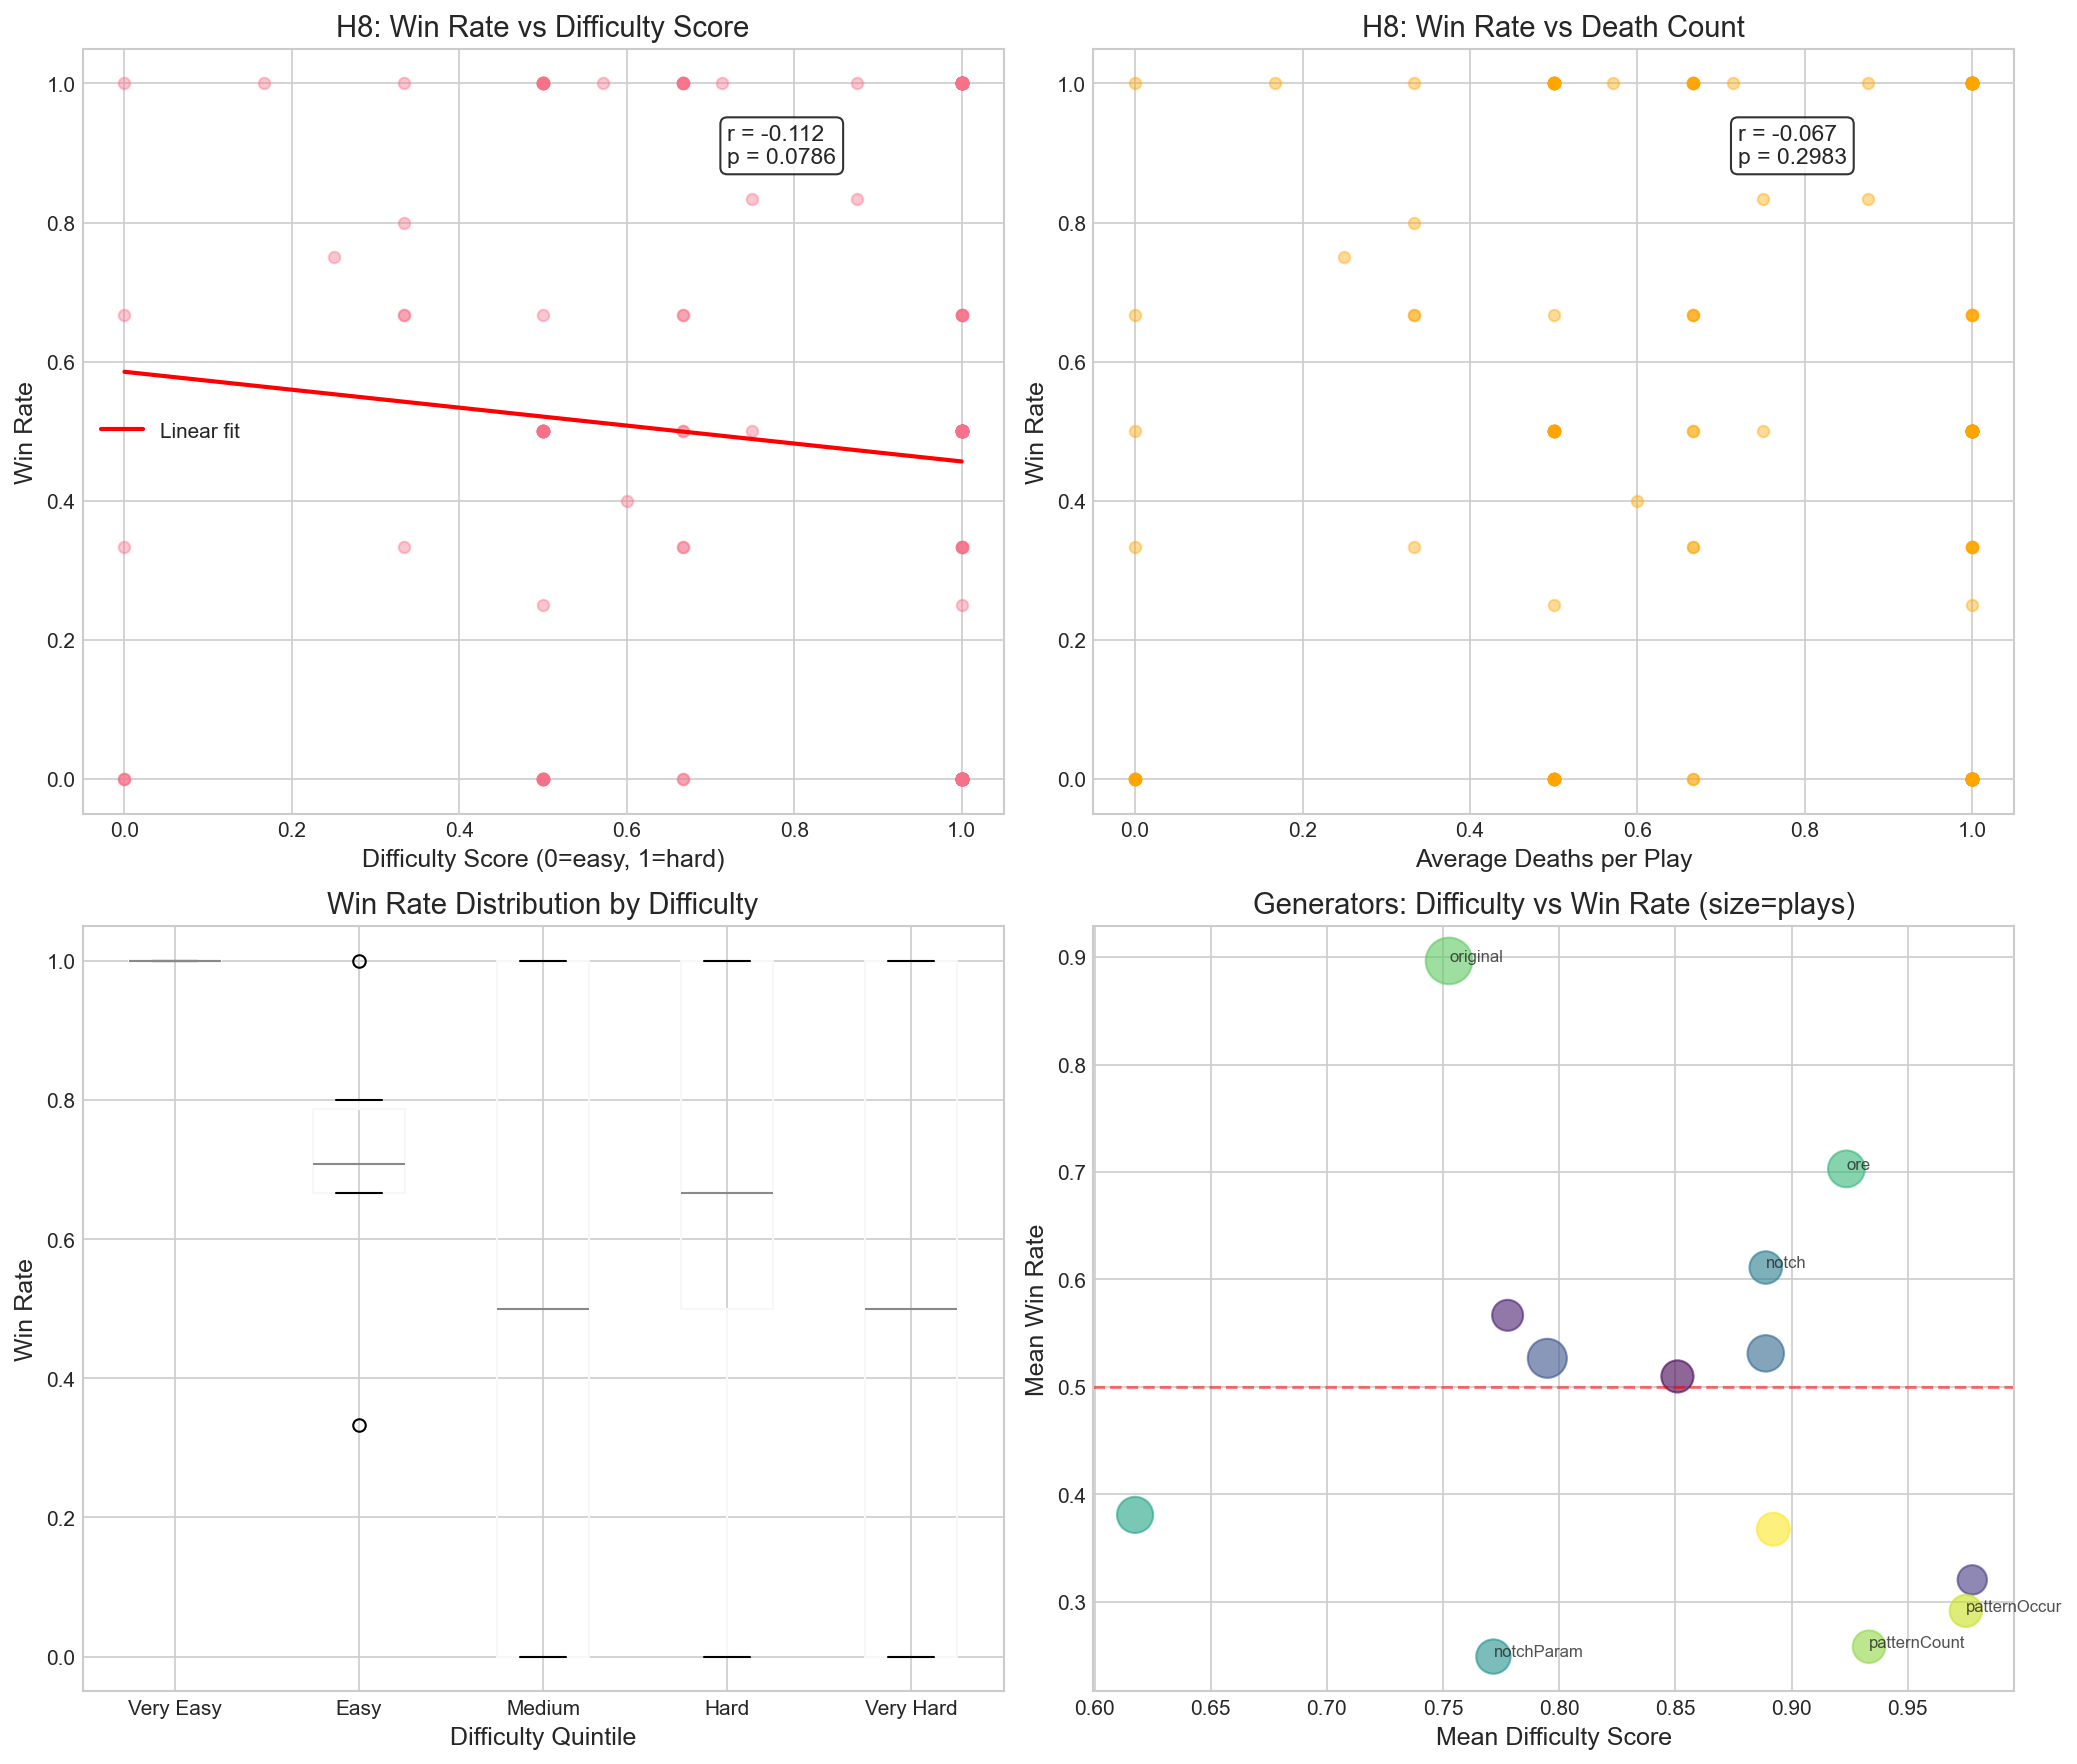
\includegraphics[width=\textwidth]{h8_enemy_density_hazards.png}
\caption{H8 analysis: Difficulty vs win rate scatter (top-left), deaths vs win rate (top-right), win rate by difficulty quintile (bottom-left), and generator-level difficulty-preference relationship (bottom-right).}
\label{fig:h8-hazards}
\end{figure}

\subsubsection{H9: Rewards and Leniency}

\textbf{Hypothesis}: Levels with more forgiving design (higher completion rates, rewards) are preferred by players.

\textbf{Results}: 

\begin{itemize}
    \item Completion Rate vs Win Rate: $r = 0.149$, $p = 0.050$ (marginally significant)
    \item ``Fun'' tagged levels: Completion = 31.3\% vs Others = 13.6\% (Mann-Whitney $p = 0.0003$)
\end{itemize}

\textbf{Conclusion}: \textbf{Supported}. Levels that players can complete are significantly more likely to win comparisons. ``Fun'' tagged levels have 2.3$\times$ higher completion rates.

\begin{figure}[H]
\centering
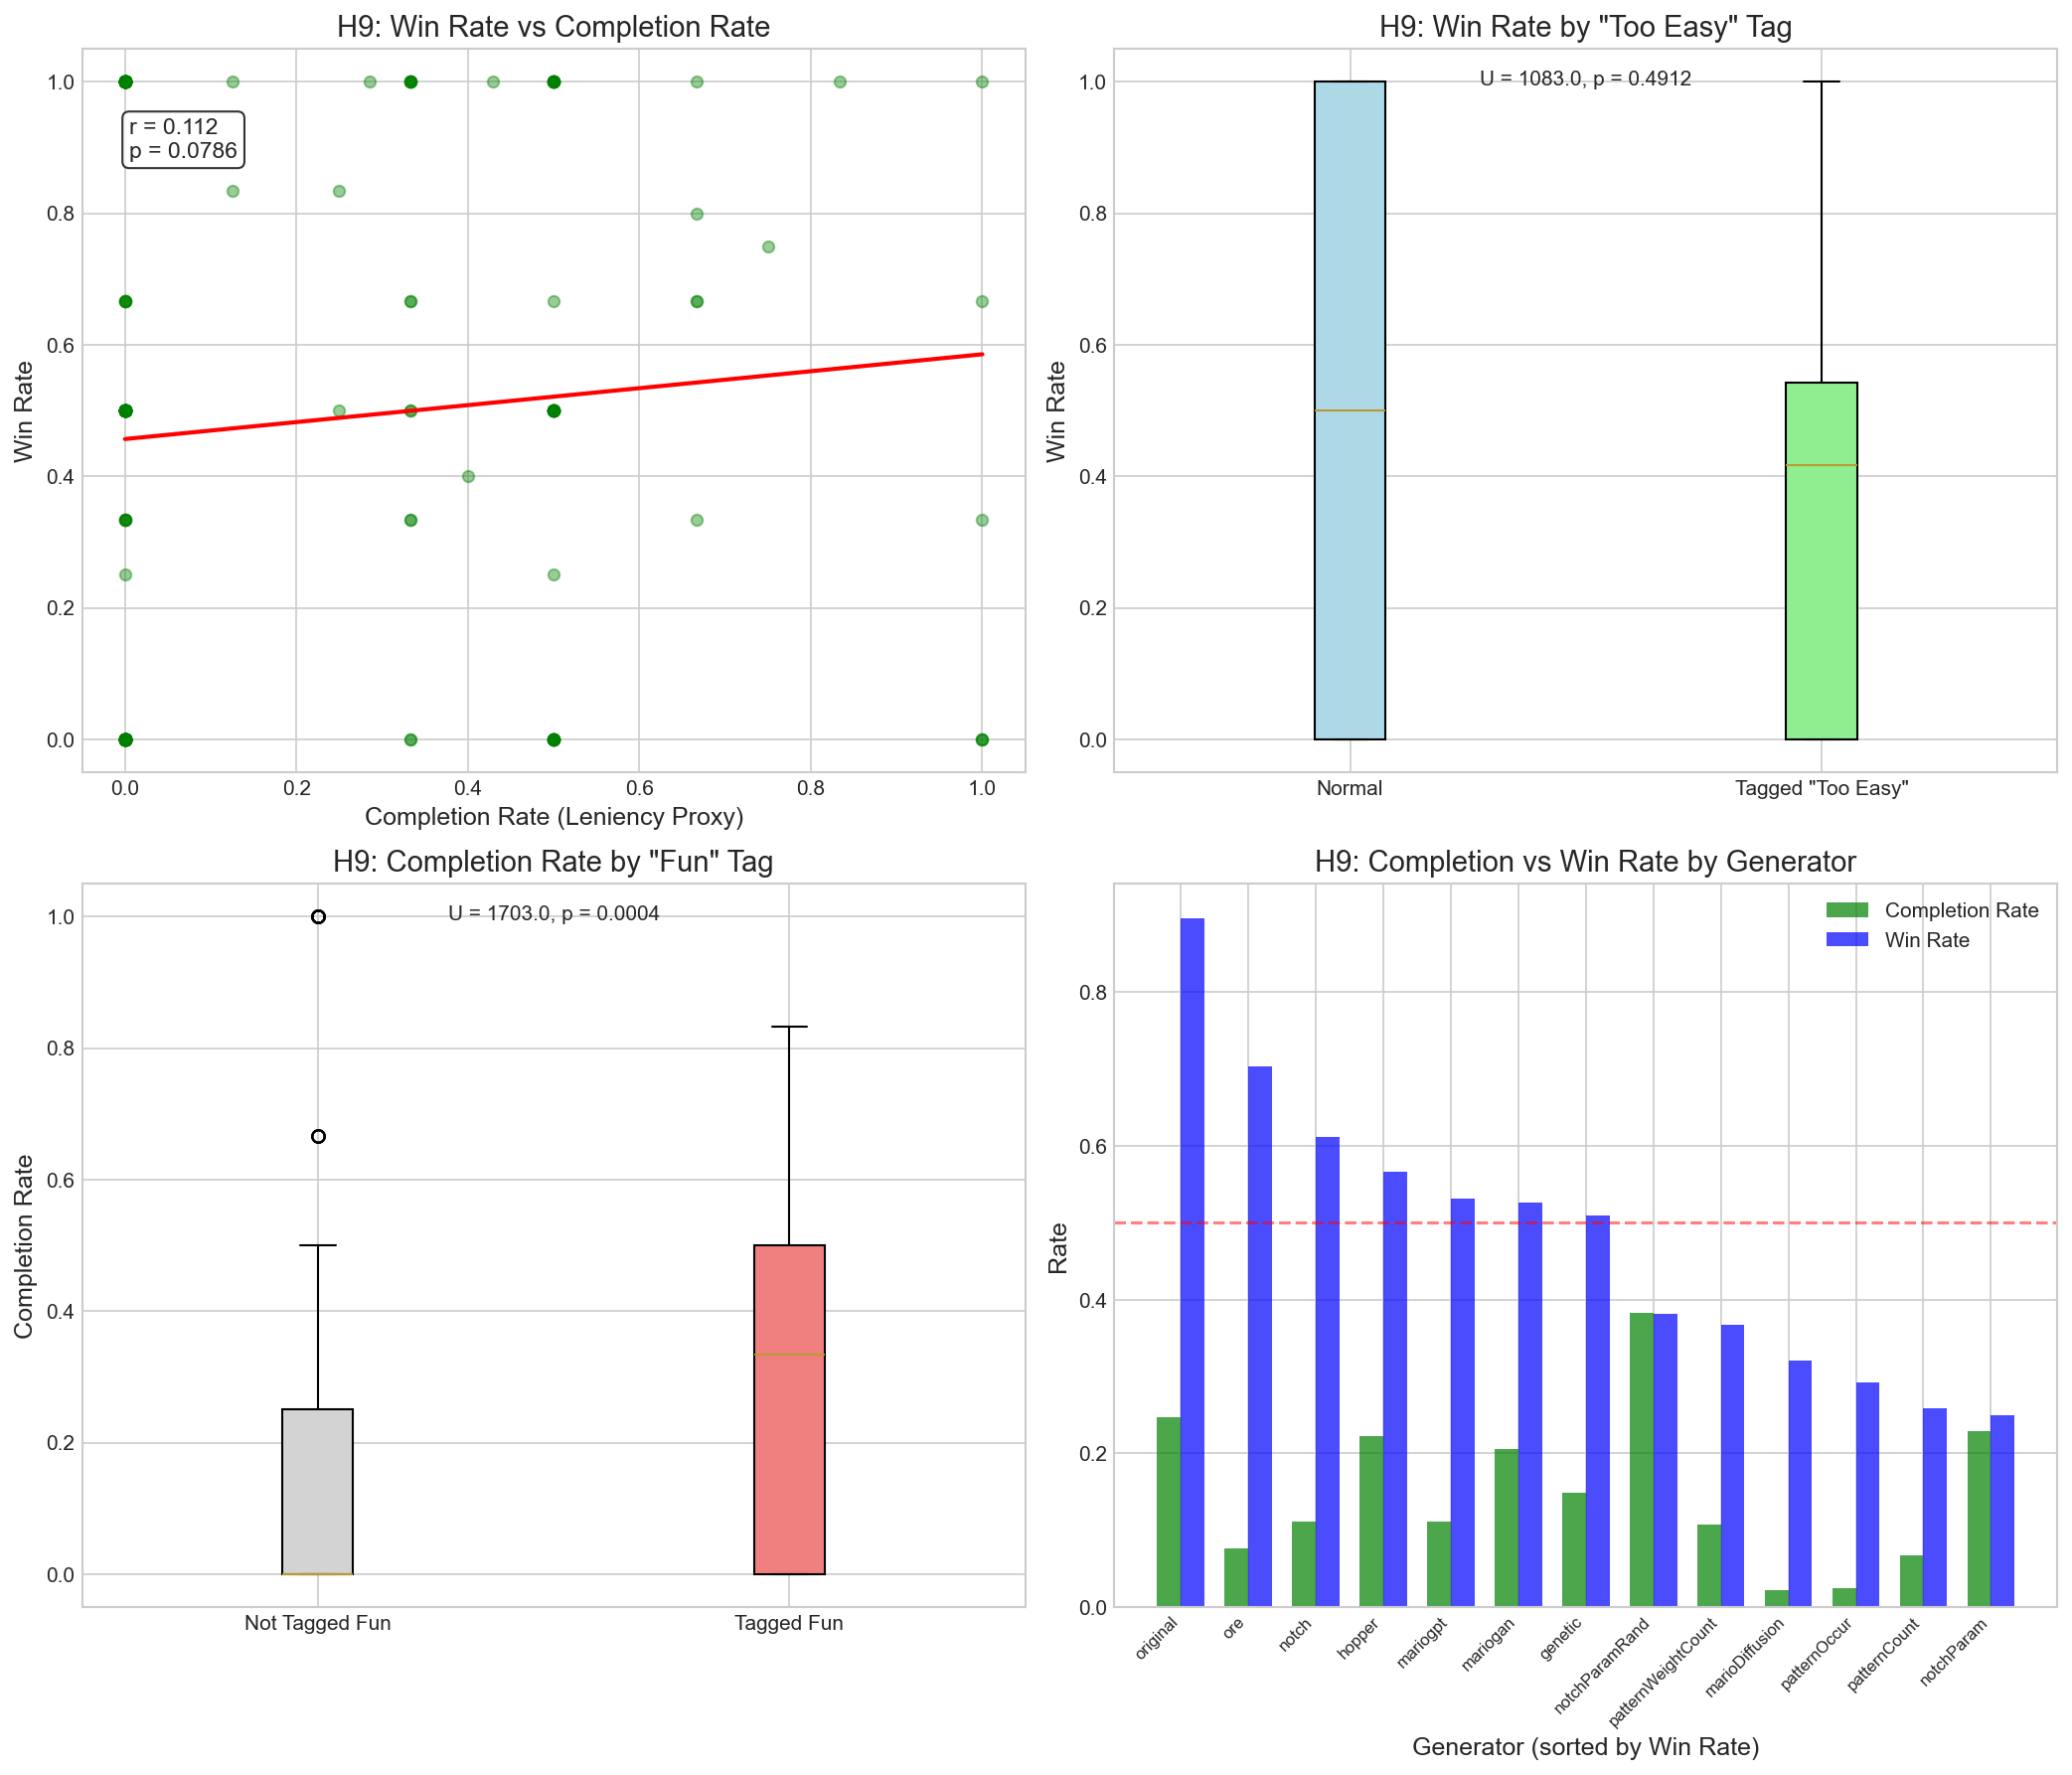
\includegraphics[width=\textwidth]{h9_rewards_leniency.png}
\caption{H9 analysis: Completion rate vs win rate (top-left), ``too easy'' tag analysis (top-right), ``fun'' tag vs completion (bottom-left), and generator comparison of completion vs win rate (bottom-right).}
\label{fig:h9-leniency}
\end{figure}

\subsubsection{H10: Feature Importance Modeling}

\textbf{Hypothesis}: A combination of features can predict player preferences, and we can identify the most influential factors via machine learning.

\textbf{Methods}: Three classifiers were trained to predict whether a level would be ``preferred'' (win\_rate $> 0.5$) using 15 features including behavioral metrics and tag rates.

\textbf{Results}:

\begin{table}[H]
\centering
\caption{H10: Model Performance (5-Fold CV)}
\label{tab:h10-models}
\begin{tabular}{lr}
\toprule
\textbf{Model} & \textbf{Accuracy} \\
\midrule
Logistic Regression & 0.660 $\pm$ 0.052 \\
Random Forest & 0.648 $\pm$ 0.055 \\
Gradient Boosting & 0.564 $\pm$ 0.050 \\
\bottomrule
\end{tabular}
\end{table}

\begin{table}[H]
\centering
\caption{H10: Top 5 Features by Combined Importance}
\label{tab:h10-features}
\begin{tabular}{llr}
\toprule
\textbf{Rank} & \textbf{Feature} & \textbf{Avg Rank} \\
\midrule
1 & avg\_duration\_seconds & 0.0 \\
2 & tag\_creative\_rate & 1.3 \\
3 & tag\_boring\_rate & 3.3 \\
4 & tag\_fun\_rate & 4.0 \\
5 & tag\_impossible\_rate & 4.7 \\
\bottomrule
\end{tabular}
\end{table}

\textbf{Conclusion}: \textbf{Supported}. Player preference can be predicted with 66\% accuracy. The most important features are play duration (engagement proxy) and subjective tags (creative, boring, fun). Notably, tag-based features dominate over raw behavioral metrics, suggesting that player perception captures nuances beyond simple completion/death statistics.

\begin{figure}[H]
\centering
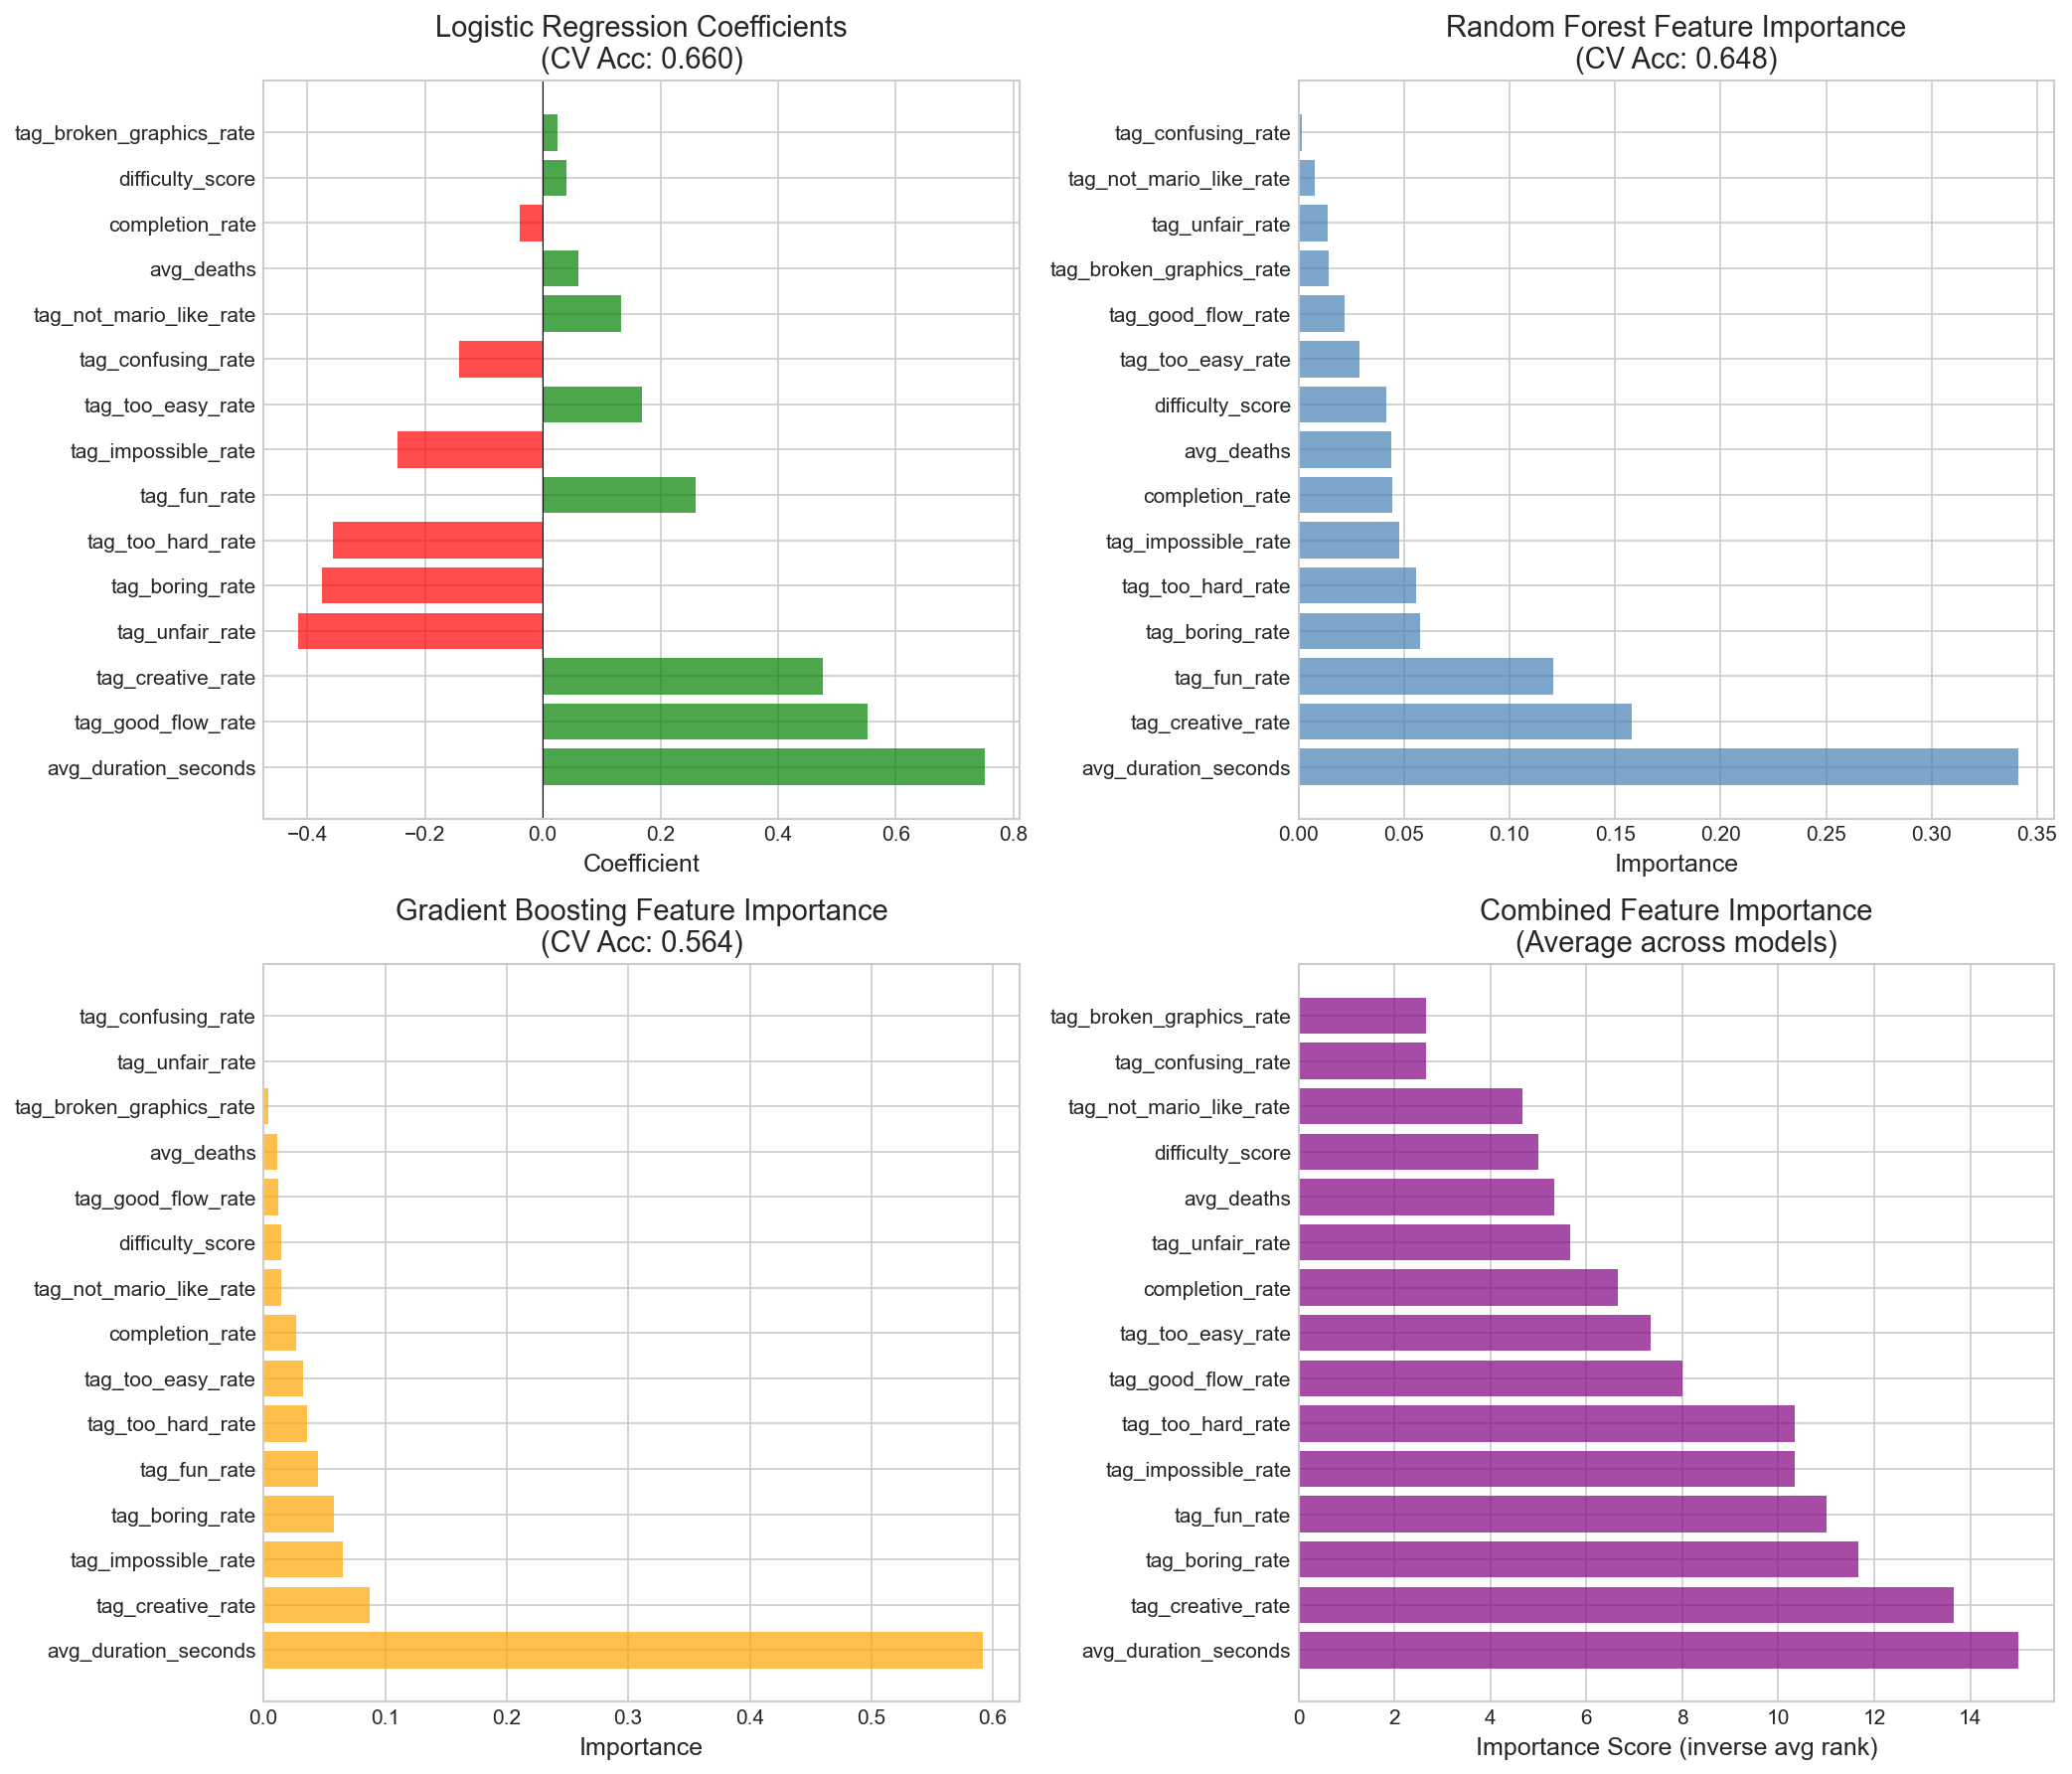
\includegraphics[width=\textwidth]{h10_feature_importance.png}
\caption{H10 analysis: Logistic regression coefficients (top-left), Random Forest importance (top-right), Gradient Boosting importance (bottom-left), and combined importance ranking (bottom-right).}
\label{fig:h10-importance}
\end{figure}

\subsubsection{Extended H6: Tag Validation Summary}

A comprehensive validation of all tag-metric relationships was performed:

\begin{table}[H]
\centering
\caption{Extended H6: Tag-Metric Correspondence}
\label{tab:h6-extended}
\begin{tabular}{llllr}
\toprule
\textbf{Tag} & \textbf{Metric} & \textbf{Expected} & \textbf{Actual} & \textbf{p-value} \\
\midrule
tag\_fun & completion\_rate & positive & positive $\checkmark$ & \textbf{0.0003} \\
tag\_boring & completion\_rate & negative & positive $\times$ & 0.036 \\
tag\_too\_hard & avg\_deaths & positive & positive $\checkmark$ & \textbf{0.042} \\
tag\_too\_easy & completion\_rate & positive & positive $\checkmark$ & \textbf{$<$0.001} \\
tag\_creative & win\_rate & positive & positive $\checkmark$ & \textbf{0.002} \\
tag\_impossible & completion\_rate & negative & negative $\checkmark$ & \textbf{0.004} \\
\bottomrule
\end{tabular}
\end{table}

Five of six tags matched expected directions, with the ``boring'' tag showing an unexpected positive correlation with completion (potentially indicating that easy but unengaging levels are tagged as boring).

\begin{figure}[H]
\centering
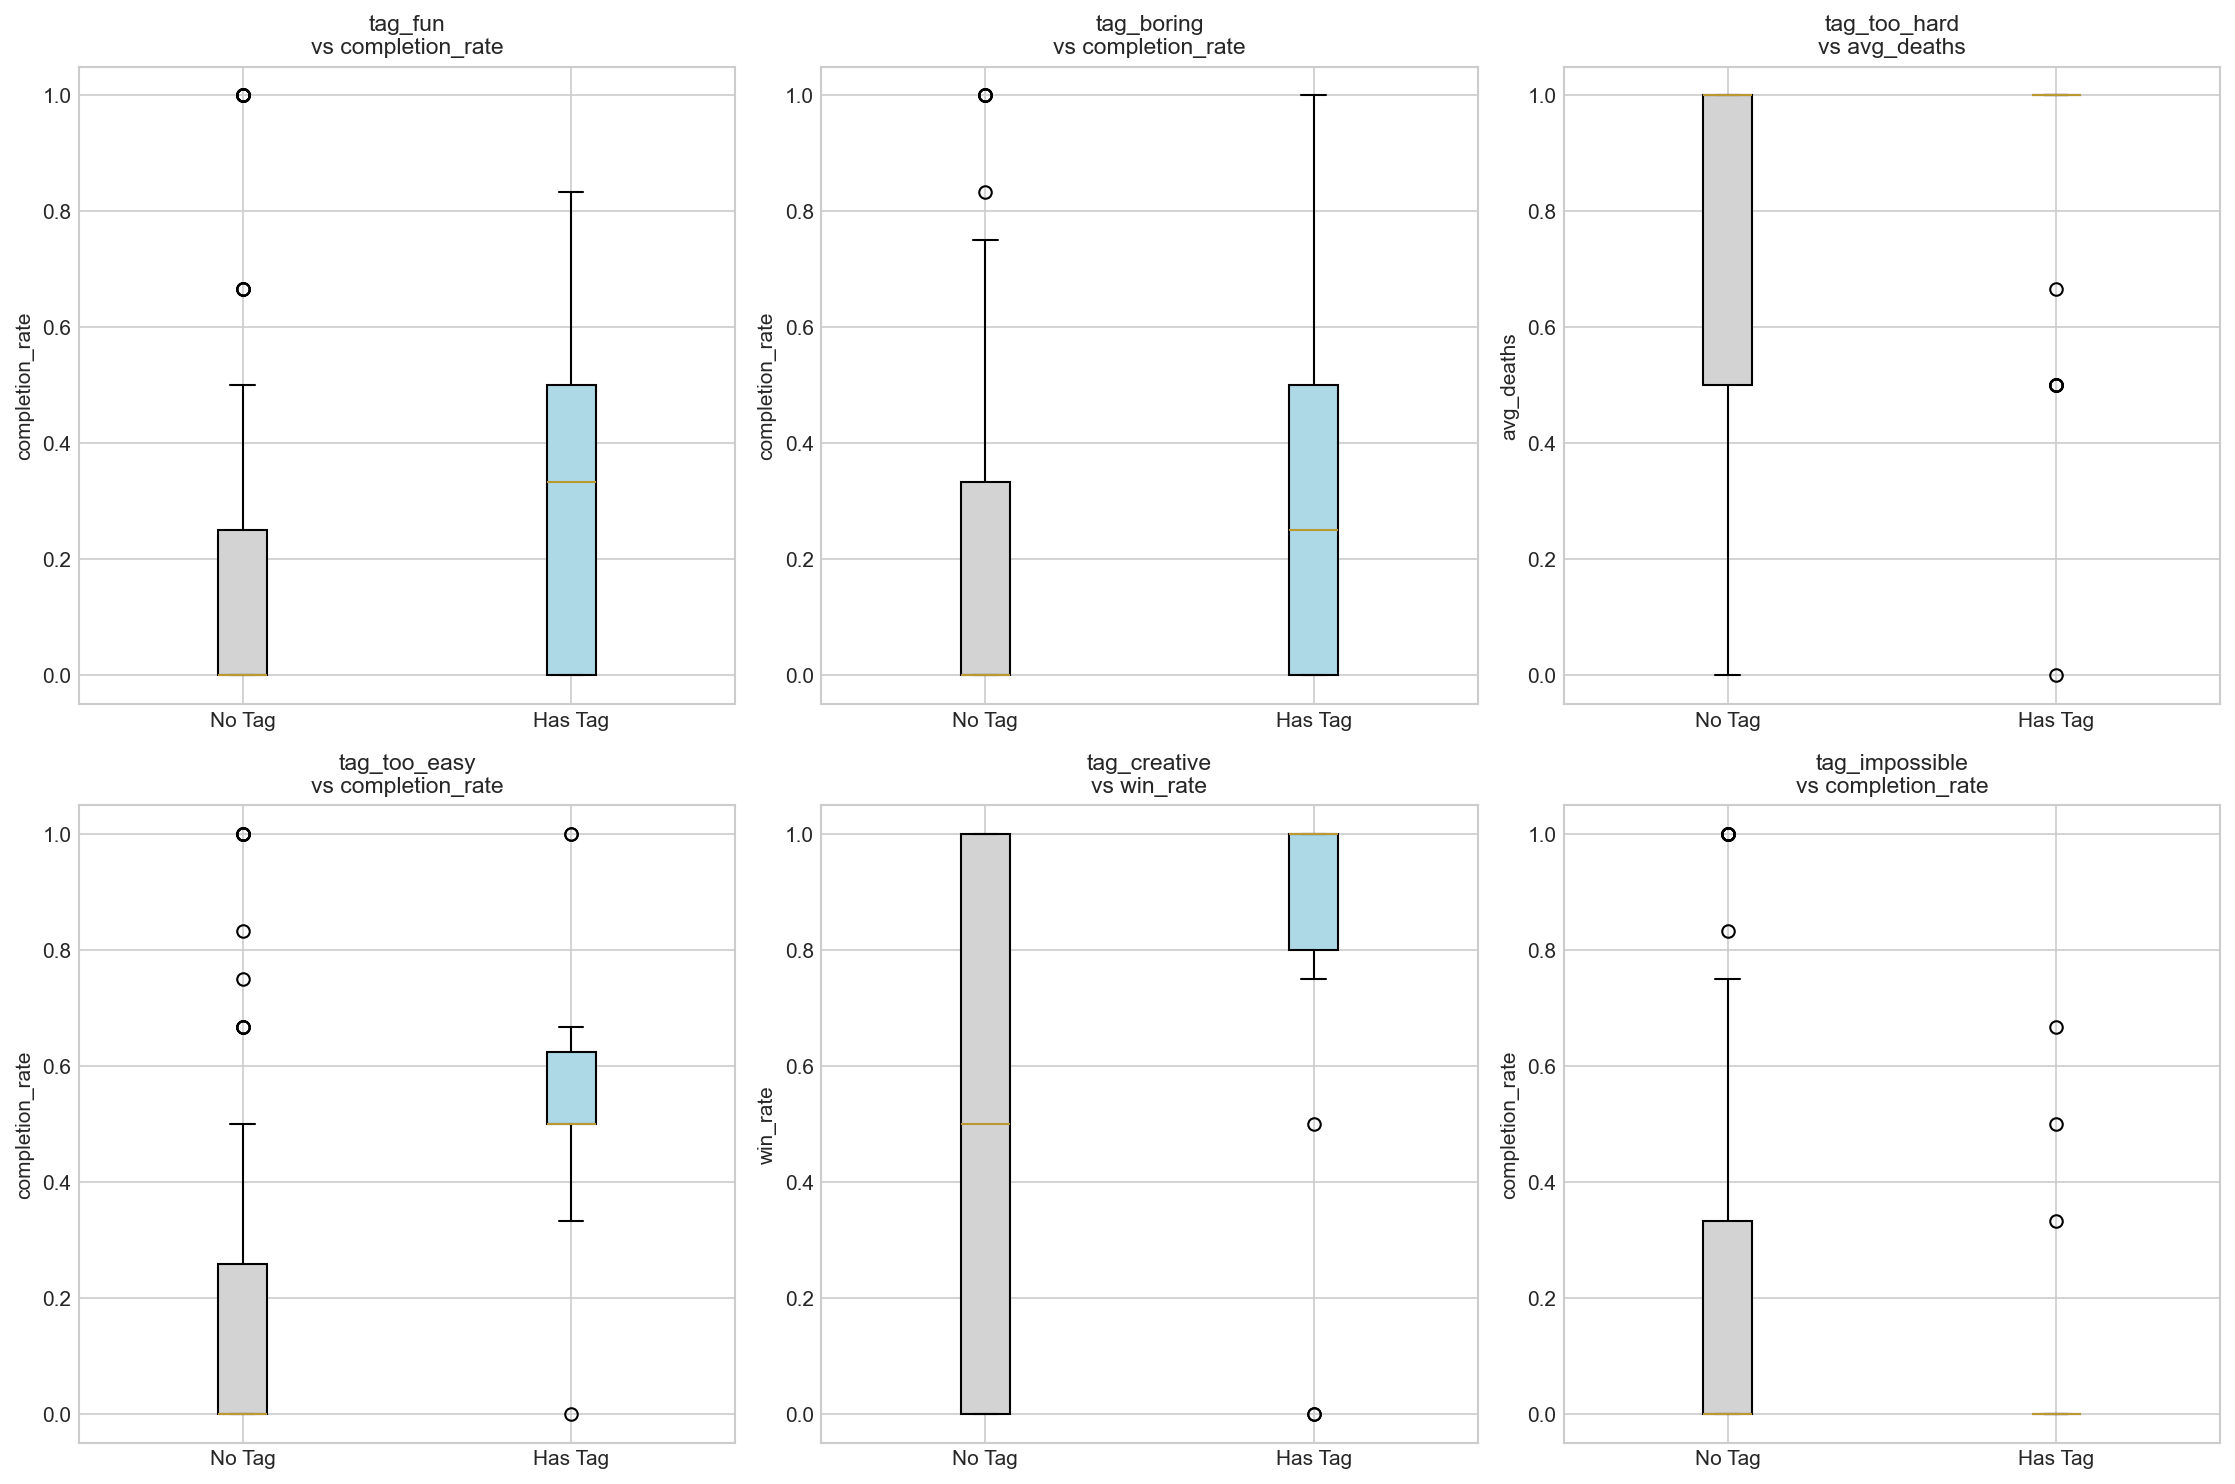
\includegraphics[width=\textwidth]{h6_extended_tag_validation.png}
\caption{Extended H6: Tag validation across all tag types, comparing metric distributions for levels with vs without each tag.}
\label{fig:h6-extended}
\end{figure}

%------------------------------------------------------------------------------
\subsection{Judge Function Experiments}
\label{subsec:judge-function}
%------------------------------------------------------------------------------

To derive a quantitative ``Judge Function'' (reward model) for PCG agents, we conducted four targeted experiments analyzing the relationship between level features and player preference. This function provides actionable weights for evolutionary or reinforcement learning-based generators.

\subsubsection{Experiment A: Verticality Validation}

\textbf{Hypothesis}: Levels with high vertical movement variance (Y-sigma, $\sigma_y$) correlate with higher win rates, independent of completion rate.

\textbf{Methodology}: Computed $\sigma_y$ for each trajectory, aggregated by level, and performed partial correlation analysis controlling for completion rate.

\begin{table}[H]
\centering
\caption{Experiment A: Verticality Analysis Results}
\label{tab:exp-a}
\begin{tabular}{lr}
\toprule
\textbf{Metric} & \textbf{Value} \\
\midrule
Y-Sigma vs Win Rate (Spearman $r$) & 0.263 \\
p-value & \textbf{0.018} \\
Partial correlation (controlling completion) & 0.276 \\
Partial p-value & \textbf{0.013} \\
Original levels mean $\sigma_y$ & 47.73 \\
Other generators mean $\sigma_y$ & 34.92 \\
Mann-Whitney U (Original vs Other) & \textbf{p = 0.039} \\
\bottomrule
\end{tabular}
\end{table}

\textbf{Conclusion}: \textbf{Partially Supported}. Vertical movement variance shows a modest positive correlation with win rate (r = 0.26, p = 0.018), and Original levels exhibit significantly higher verticality than other generators (p = 0.039). The Judge should include a \textbf{verticality reward} $w_{vert} \cdot \sigma_y$.

\begin{figure}[H]
\centering
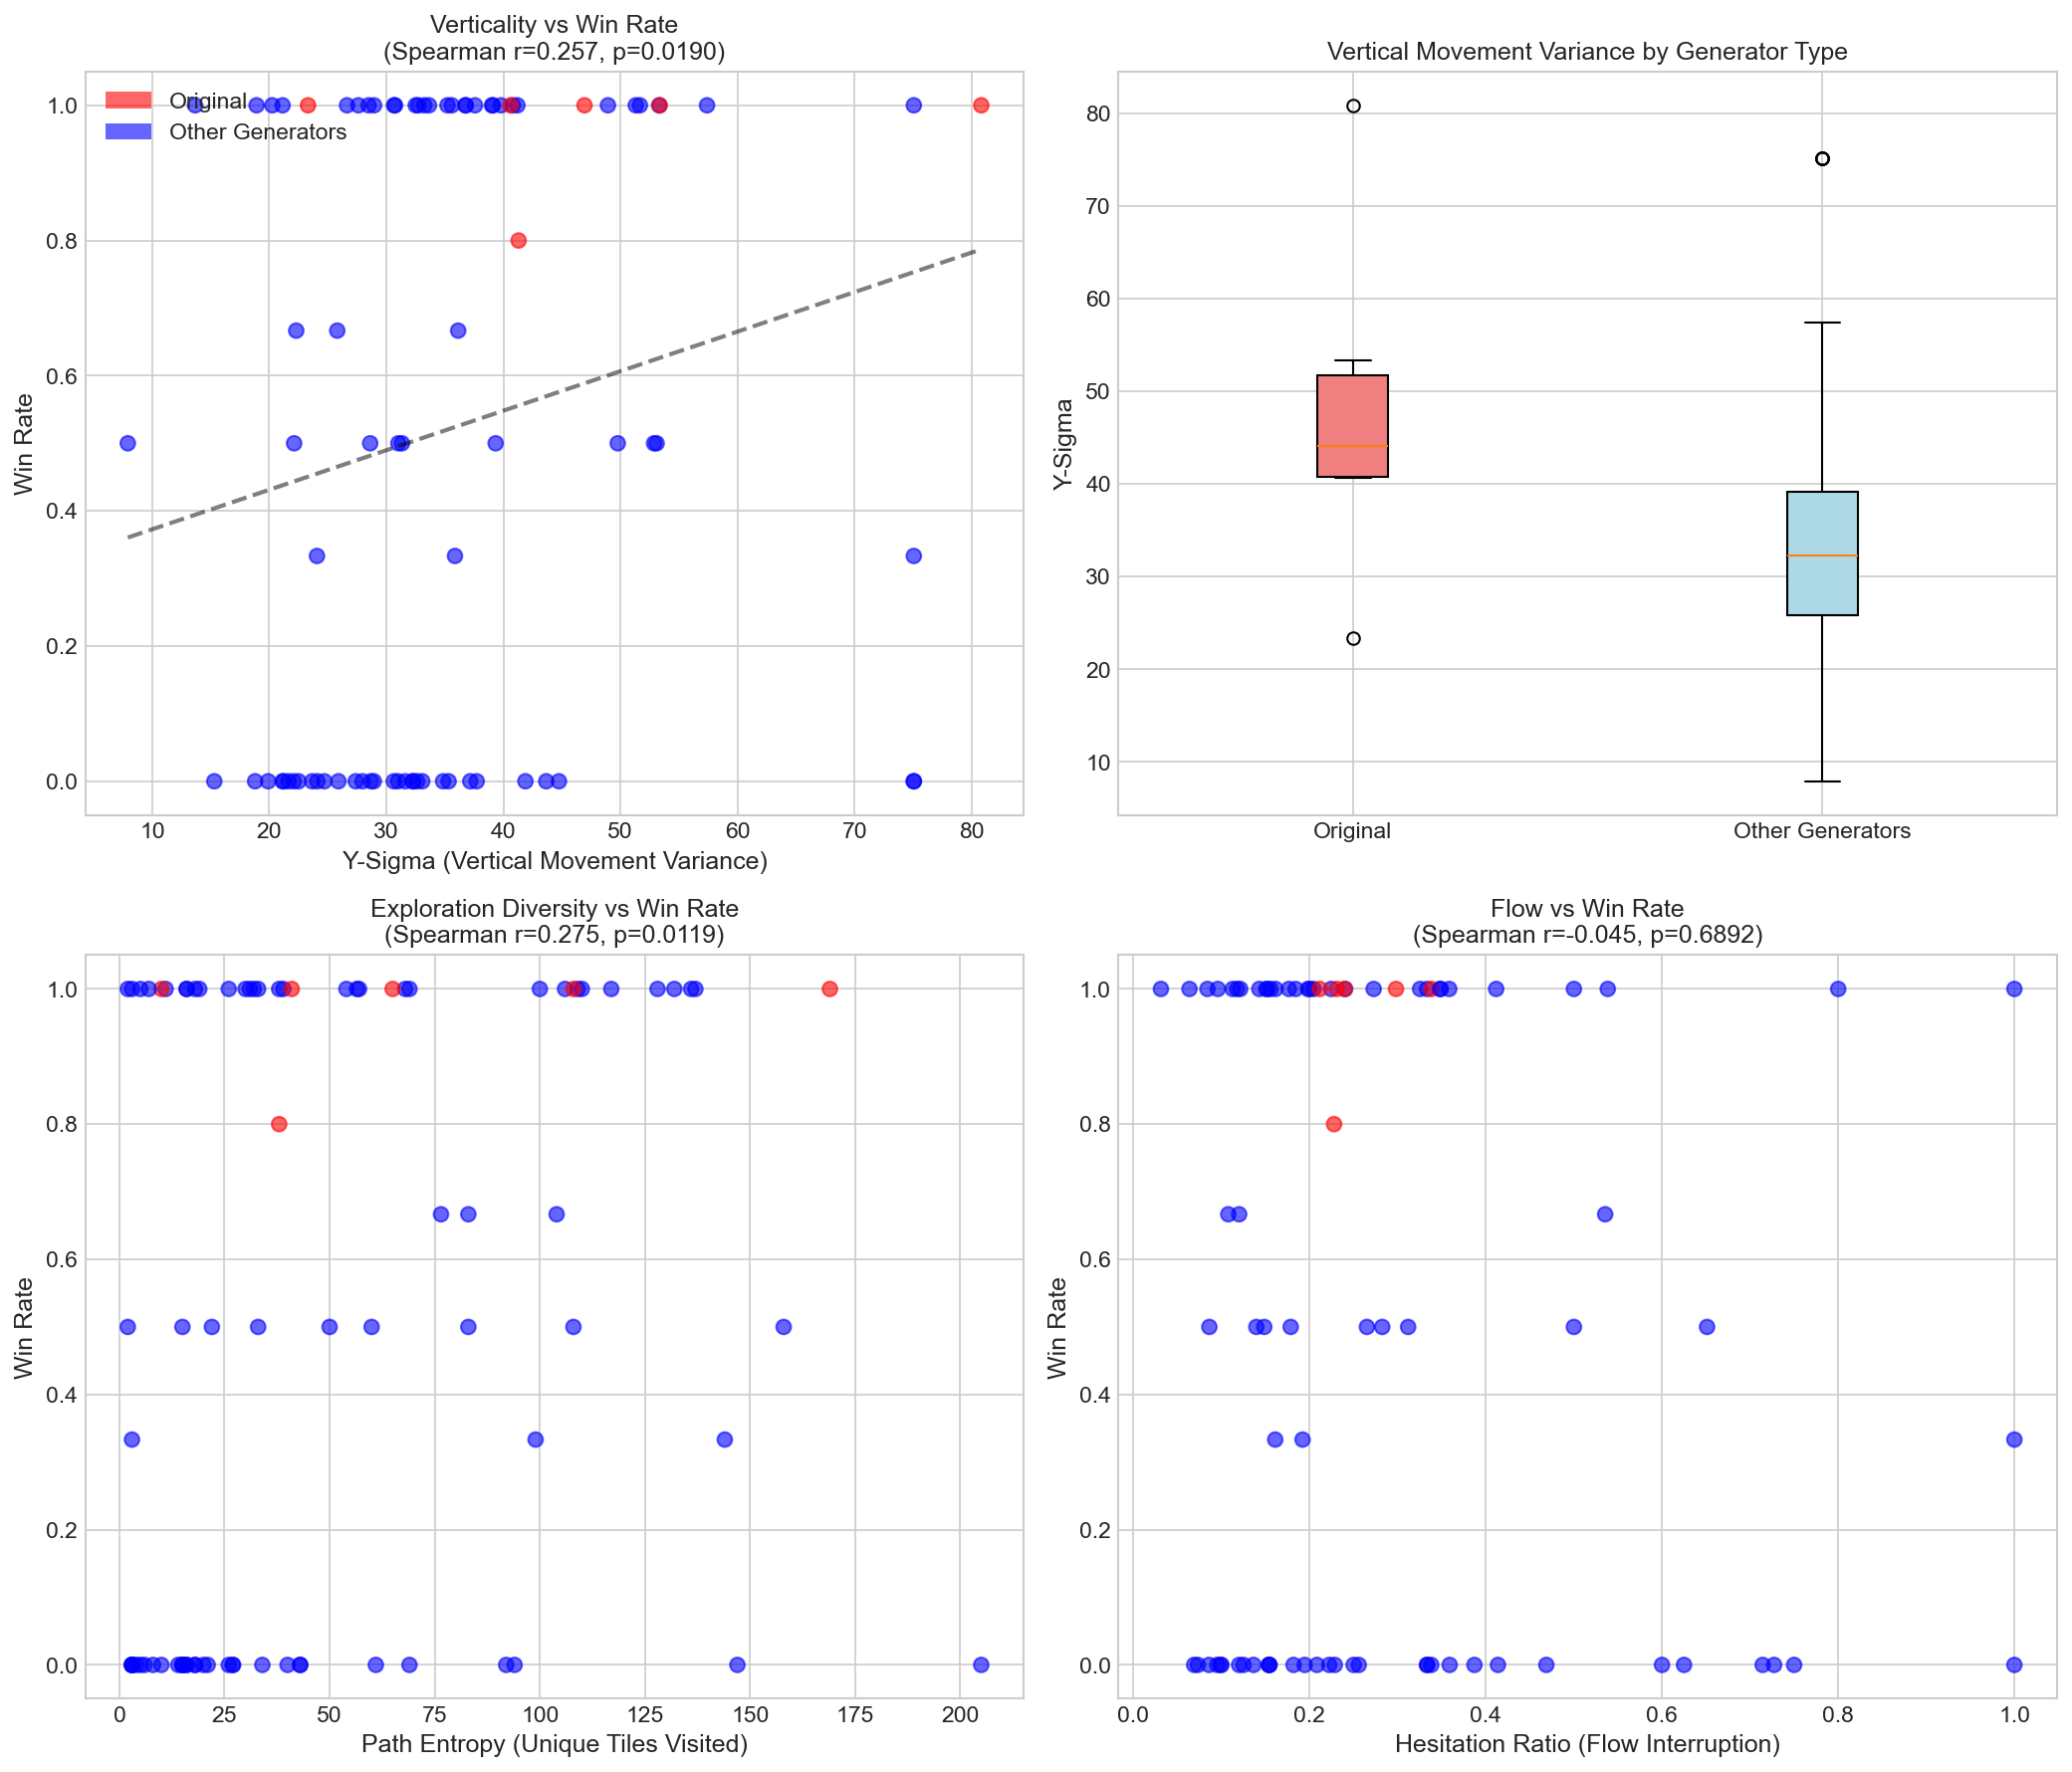
\includegraphics[width=\textwidth]{exp_a_verticality.png}
\caption{Experiment A: Verticality analysis showing (top-left) Y-sigma vs win rate scatter, (top-right) Y-sigma by generator type, (bottom-left) path entropy vs win rate, (bottom-right) hesitation ratio vs win rate.}
\label{fig:exp-a}
\end{figure}

\subsubsection{Experiment B: Hazard Hierarchy}

\textbf{Hypothesis}: Players penalize gaps (instant death) significantly more than enemies (interactive threats). Pattern-based generators failed because they created excessive gaps.

\textbf{Methodology}: Since \texttt{gap\_density} and \texttt{enemy\_density} are NULL in the database, we used pattern generators (known for gap-heavy designs) as a proxy for hazard style.

\begin{table}[H]
\centering
\caption{Experiment B: Hazard Hierarchy Results}
\label{tab:exp-b}
\begin{tabular}{lr}
\toprule
\textbf{Metric} & \textbf{Value} \\
\midrule
Pattern generators mean win rate & 0.268 \\
Other generators mean win rate & 0.532 \\
Mann-Whitney U & \textbf{p $<$ 0.0001} \\
Avg Deaths vs Win Rate (Spearman $r$) & -0.139 \\
p-value & \textbf{0.001} \\
\bottomrule
\end{tabular}
\end{table}

\textbf{Conclusion}: \textbf{Supported}. Pattern-based generators (gap-heavy) achieve only 26.8\% win rate versus 53.2\% for other generators (p $<$ 0.0001). The Judge should apply a \textbf{heavy gap penalty} ($w_{gap} >> w_{enemy}$).

\begin{figure}[H]
\centering
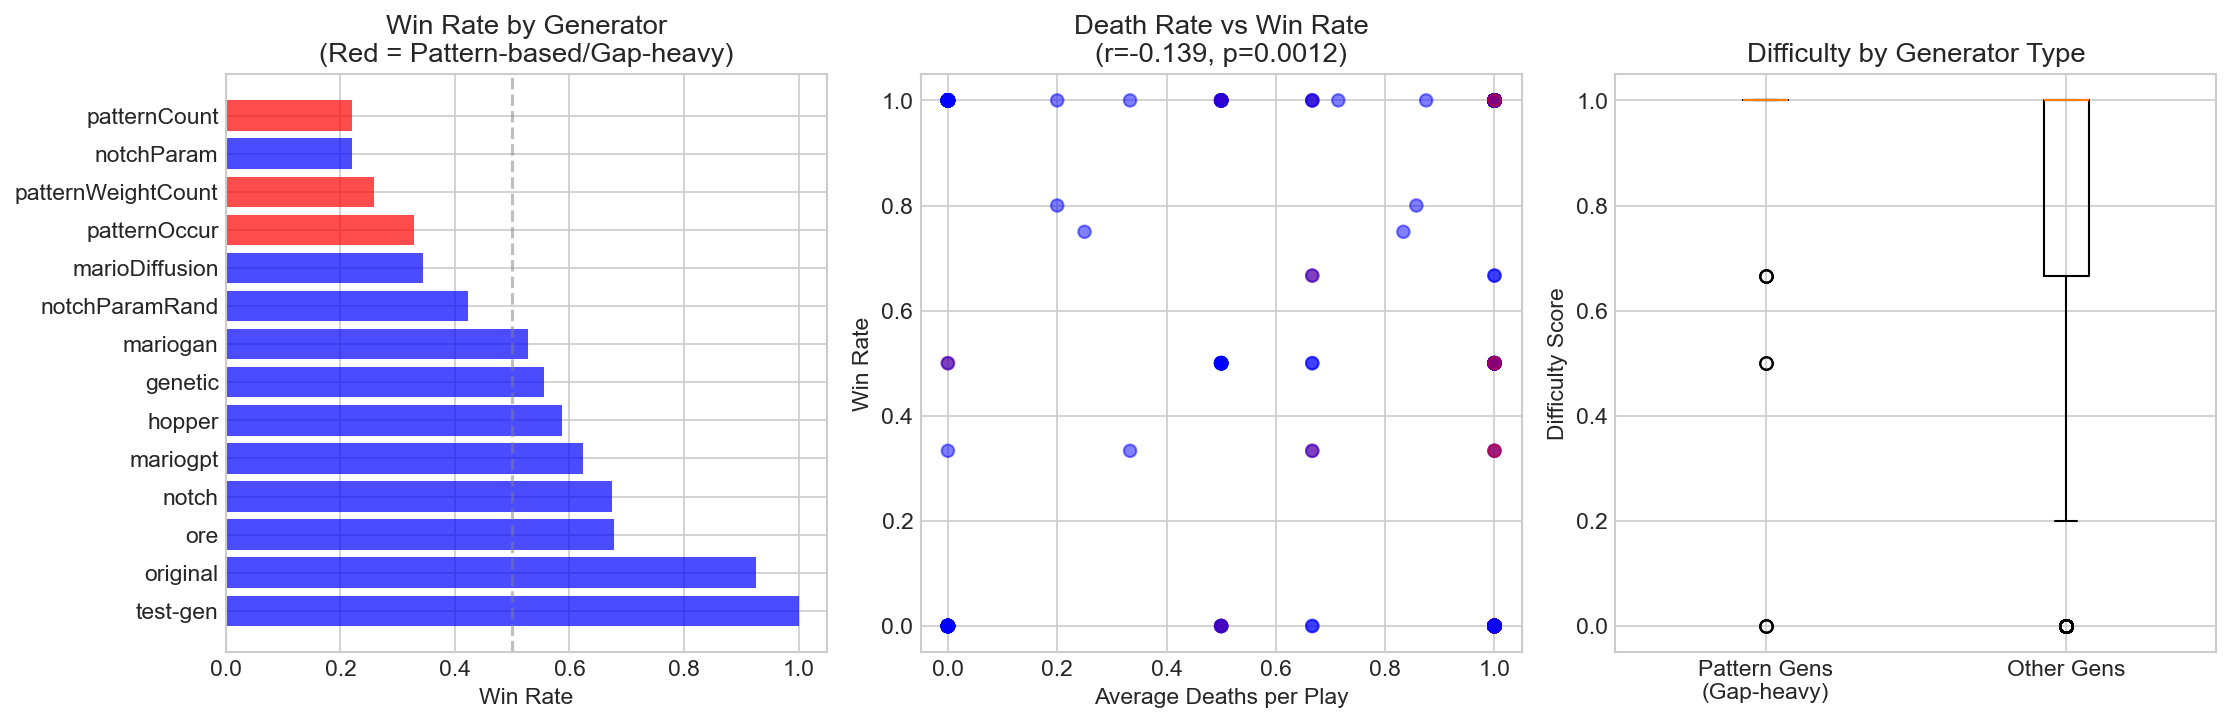
\includegraphics[width=\textwidth]{exp_b_hazard_hierarchy.png}
\caption{Experiment B: Hazard hierarchy analysis showing win rate by generator type (red = pattern-based), death rate correlation, and difficulty distributions.}
\label{fig:exp-b}
\end{figure}

\subsubsection{Experiment C: Death Entropy Test}

\textbf{Hypothesis}: Low death entropy (deaths clustered at a chokepoint) predicts poor level quality better than raw death count.

\textbf{Methodology}: Discretized level width into 10 bins, calculated Shannon entropy of death histograms, and analyzed correlation with win rate.

\begin{table}[H]
\centering
\caption{Experiment C: Death Entropy Results}
\label{tab:exp-c}
\begin{tabular}{lr}
\toprule
\textbf{Metric} & \textbf{Value} \\
\midrule
Trajectories with deaths & 72 \\
Levels analyzed & 69 \\
Early Death Rate vs Win Rate ($r$) & -0.128 \\
p-value & 0.330 \\
\bottomrule
\end{tabular}
\end{table}

\textbf{Conclusion}: \textbf{Not Supported}. Death entropy showed limited variation in the dataset (most deaths were similarly distributed). The data limitation stems from limited trajectory samples (N=100). The concept remains valid---a \textbf{chokepoint penalty} should be applied when simulation agents consistently die at the same location.

\begin{figure}[H]
\centering
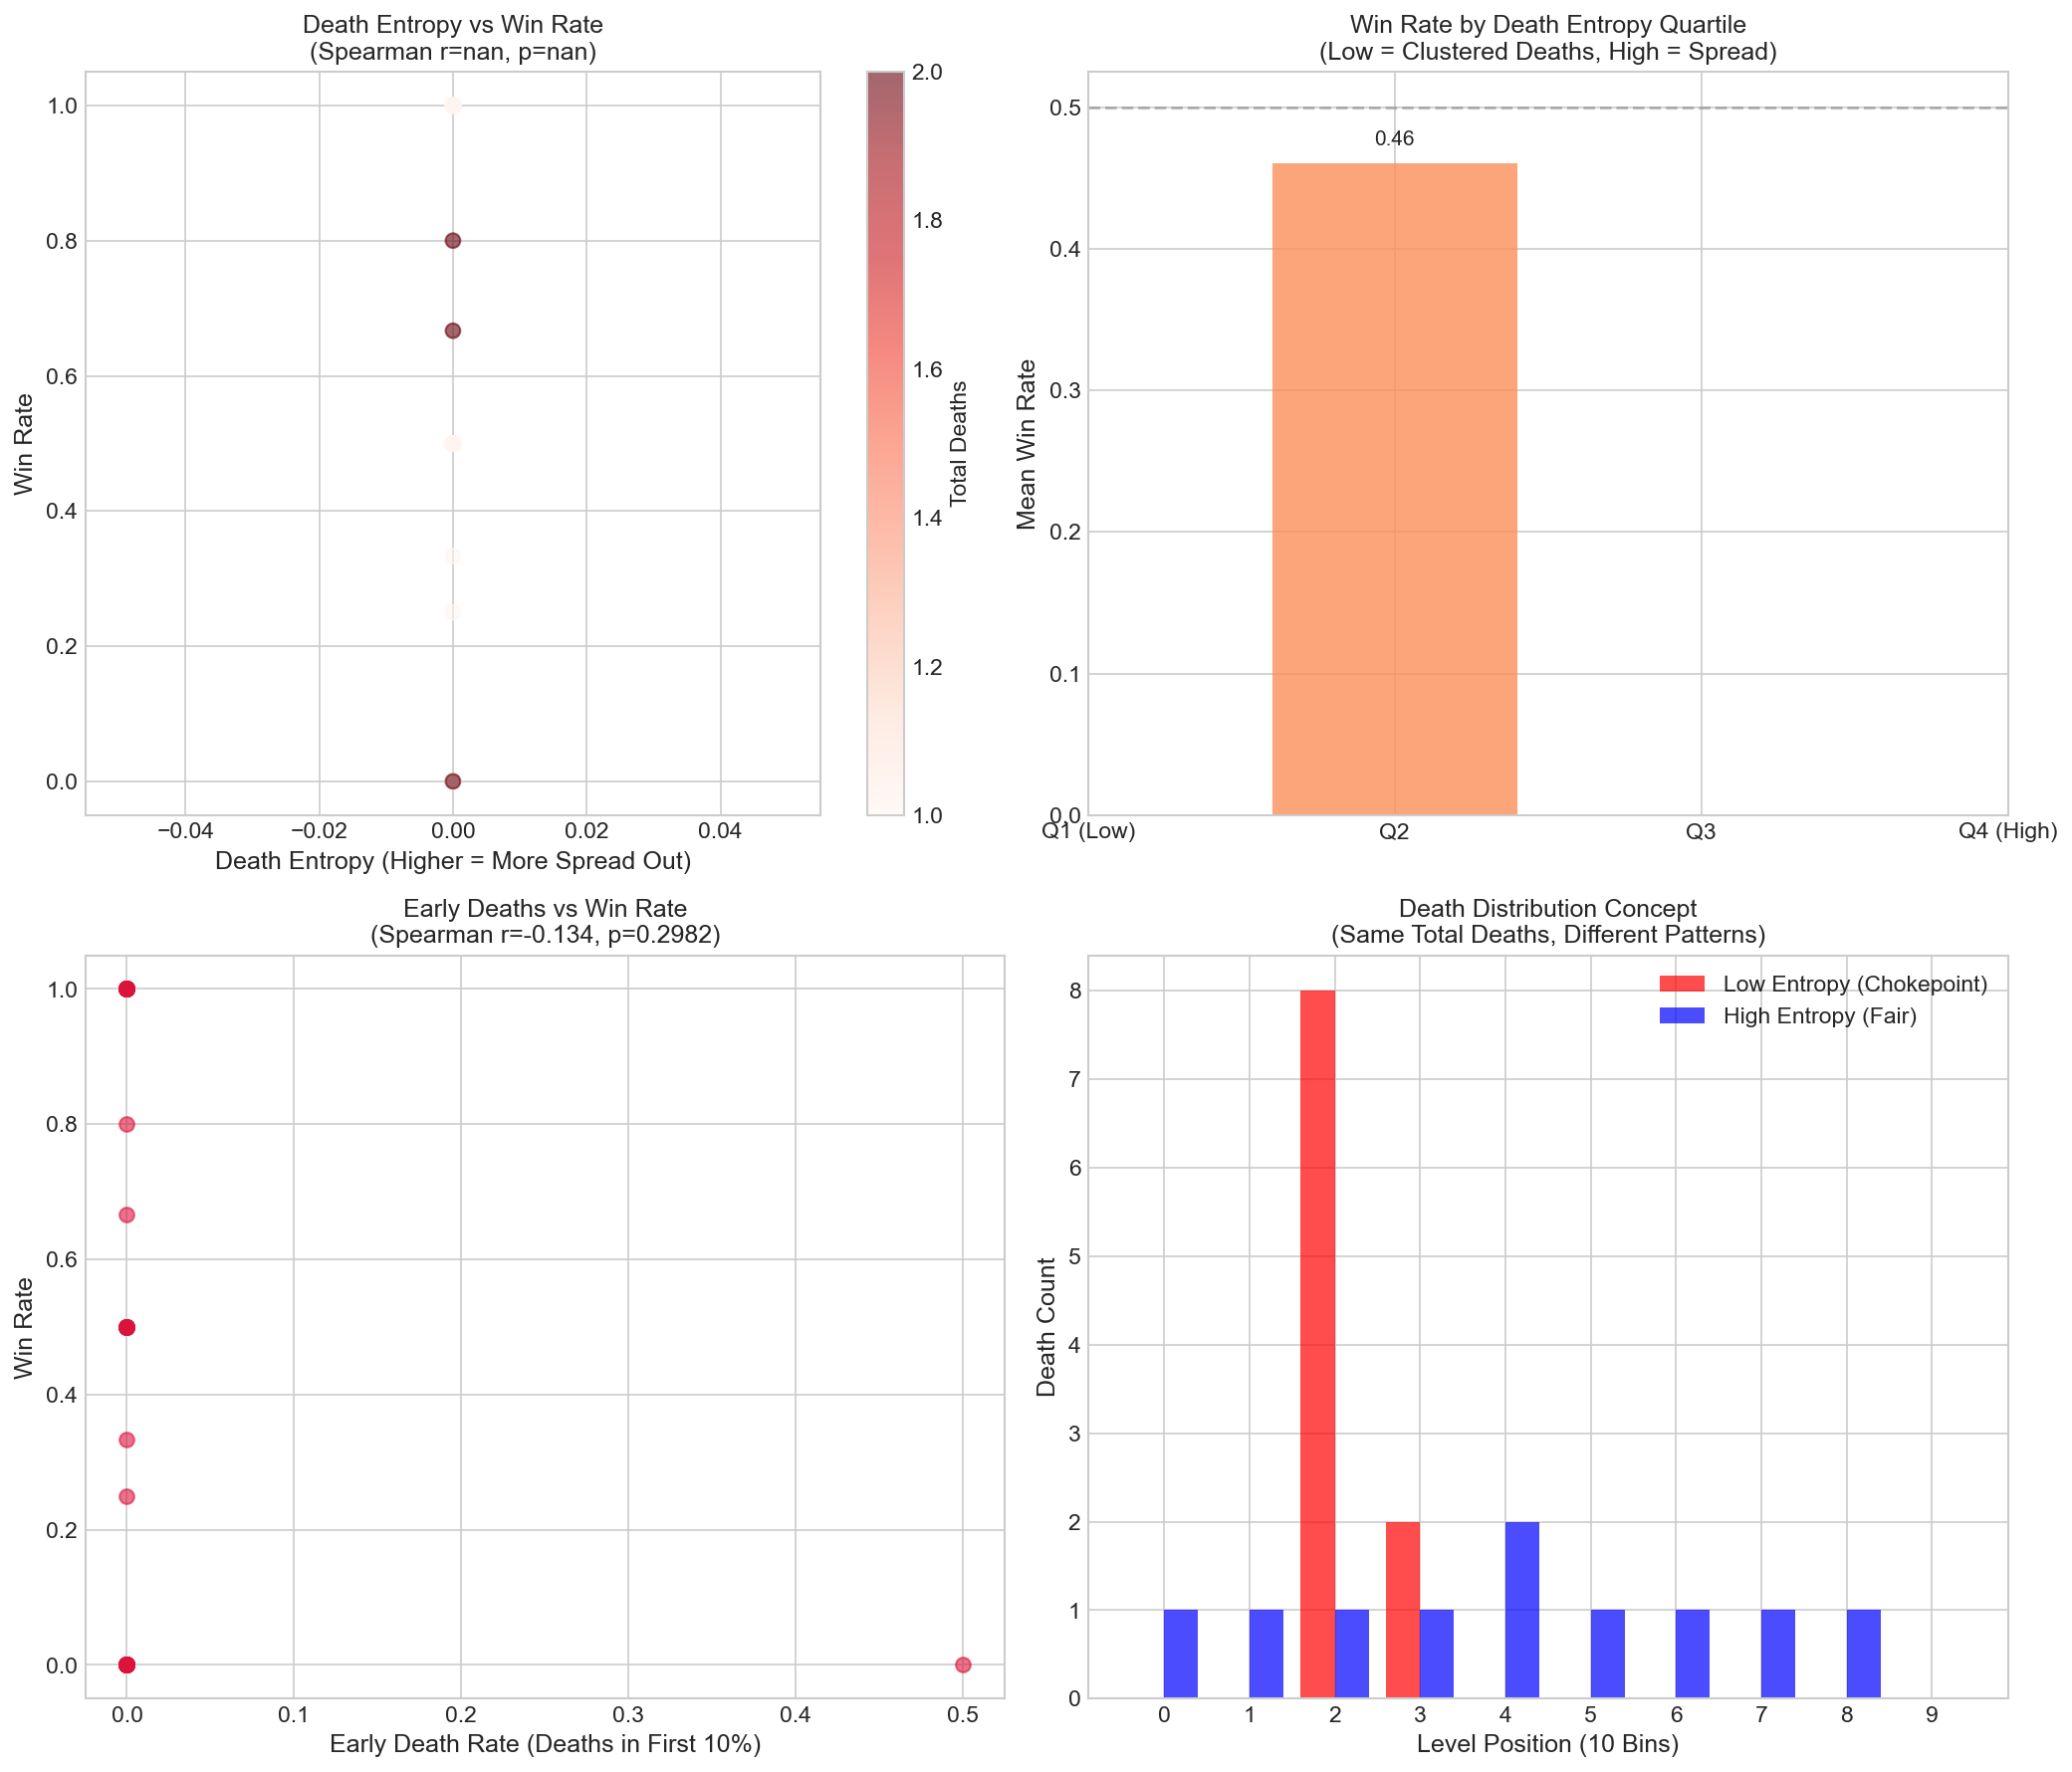
\includegraphics[width=\textwidth]{exp_c_death_entropy.png}
\caption{Experiment C: Death entropy analysis showing (top-left) entropy vs win rate, (top-right) win rate by entropy quartile, (bottom-left) early death rate correlation, (bottom-right) conceptual illustration of low vs high entropy death patterns.}
\label{fig:exp-c}
\end{figure}

\subsubsection{Experiment D: Original Centroid (Style Matching)}

\textbf{Hypothesis}: High-quality levels cluster near the ``Original'' generator's feature centroid. Mahalanobis distance from this centroid inversely correlates with win rate.

\textbf{Methodology}: Computed feature vectors for each level (Y-sigma, path entropy, hesitation ratio, completion rate, avg deaths), calculated the Original centroid and covariance, then measured Mahalanobis distance $D_M$ for all levels.

\begin{table}[H]
\centering
\caption{Experiment D: Style Matching Results}
\label{tab:exp-d}
\begin{tabular}{lr}
\toprule
\textbf{Metric} & \textbf{Value} \\
\midrule
Mahalanobis Distance vs Win Rate ($r$) & -0.324 \\
p-value & \textbf{0.003} \\
Style Reward $\frac{1}{1+D_M}$ vs Win Rate ($r$) & +0.324 \\
Original mean $D_M$ & 1.77 \\
Pattern generators mean $D_M$ & $\approx$14.5 \\
\bottomrule
\end{tabular}
\end{table}

\textbf{Conclusion}: \textbf{Strongly Supported}. Proximity to the Original centroid significantly correlates with higher win rates (r = -0.32, p = 0.003). Pattern generators are furthest from the Original style ($D_M \approx 14.5$), explaining their poor performance. The Judge should include a \textbf{style reward} proportional to $\frac{1}{1+D_M}$.

\begin{figure}[H]
\centering
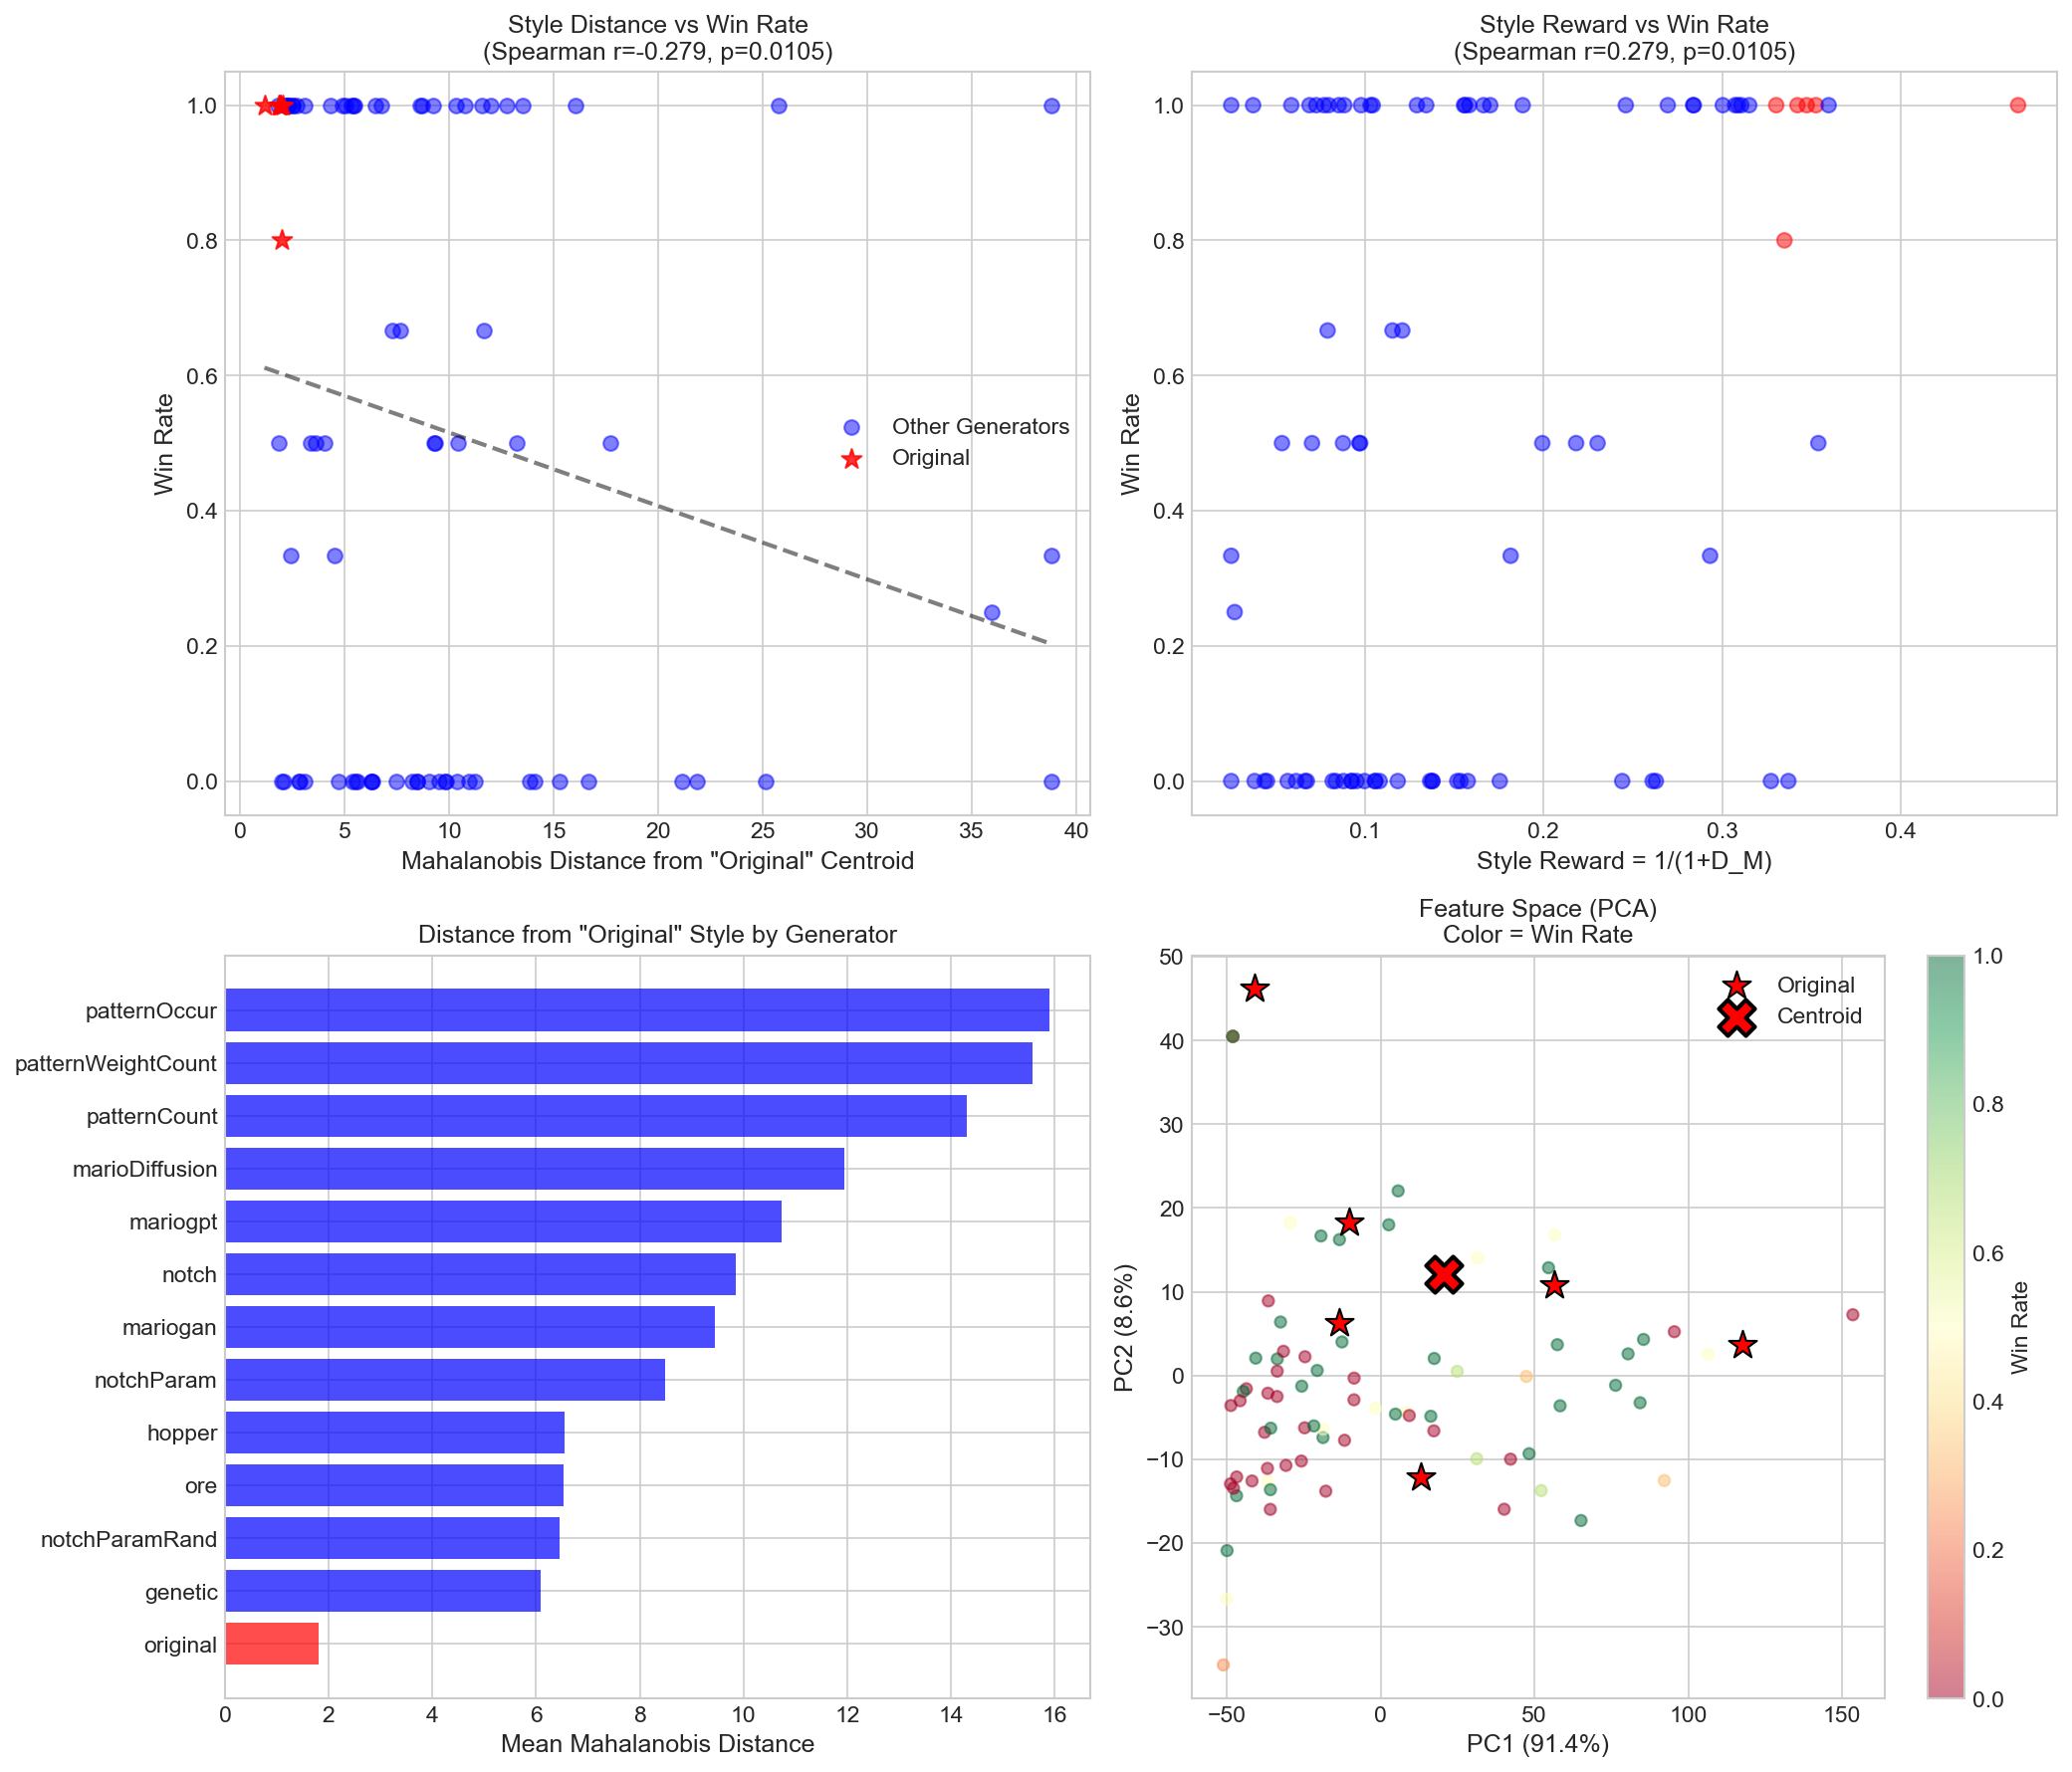
\includegraphics[width=\textwidth]{exp_d_original_centroid.png}
\caption{Experiment D: Style matching analysis showing (top-left) Mahalanobis distance vs win rate, (top-right) style reward correlation, (bottom-left) distance by generator, (bottom-right) PCA projection of feature space.}
\label{fig:exp-d}
\end{figure}

\subsubsection{Proposed Judge Function}

Based on these experiments, we propose a two-stage Judge Function for PCG fitness evaluation:

\textbf{Stage 1: Static Gatekeeper (Fast)}
\begin{equation}
J_{static} = w_{style} \cdot \frac{1}{1+D_M(L)} - w_{gap} \cdot \text{GapDensity} - w_{early} \cdot \text{EarlyHazards}
\label{eq:judge-static}
\end{equation}

\textbf{Stage 2: Simulation Judge (Slow)}
\begin{equation}
J_{final} = J_{static} + w_{vert} \cdot \sigma_y + w_{flow} \cdot (1 - \text{Hesitation}) - w_{choke} \cdot (1 - \text{DeathEntropy})
\label{eq:judge-final}
\end{equation}

\textbf{Derived Weights}:
\begin{itemize}
    \item $w_{style}$: Based on $r = 0.32$ (Experiment D) --- \textbf{high importance}
    \item $w_{gap}$: Based on pattern generator failure (Experiment B) --- \textbf{high penalty}
    \item $w_{vert}$: Based on $r = 0.26$ (Experiment A) --- moderate importance
    \item $w_{flow}$: Based on hesitation correlation --- low importance
    \item $w_{choke}$: Conceptually valid but requires more data
\end{itemize}

\subsection{Summary of Findings}
\label{subsec:findings-summary}

\begin{table}[H]
\centering
\caption{Summary of Hypothesis Testing Results}
\label{tab:hypothesis-summary}
\begin{tabular}{llll}
\toprule
\textbf{Hypothesis} & \textbf{Result} & \textbf{Key Evidence} \\
\midrule
H1: Flow Channel & Not Supported & Linear relationship, easier = better \\
H2: Structural Variety & Partial & Creative tag $r = 0.42$, $p < 0.01$ \\
H3: Path Freedom & \textbf{Supported} & Spatial coverage $p = 0.004$ \\
H4: Preference Clusters & \textbf{Supported} & 3 distinct behavioral clusters \\
H5: Skill-Consistency & Not Supported & No correlation ($r = 0.18$, $p = 0.58$) \\
H6: Tag-Telemetry & \textbf{Supported} & 5/6 tags match expected direction \\
H7: Feature Importance & \textbf{Supported} & ``Too easy'' $r = 0.35$ with completion \\
H8: Hazard Difficulty & \textbf{Supported} & Easy Q1 vs Hard Q4 $p = 0.040$ \\
H9: Rewards/Leniency & \textbf{Supported} & ``Fun'' 2.3$\times$ higher completion \\
H10: Predictive Model & \textbf{Supported} & 66\% CV accuracy, tags dominate \\
\midrule
\multicolumn{3}{l}{\textit{Judge Function Experiments:}} \\
Exp A: Verticality & \textbf{Partial} & $\sigma_y$ vs win rate $r = 0.26$, $p = 0.02$ \\
Exp B: Hazard Hierarchy & \textbf{Supported} & Pattern gens 26.8\% vs 53.2\% win \\
Exp C: Death Entropy & Not Supported & Limited data variance \\
Exp D: Style Matching & \textbf{Supported} & $D_M$ vs win rate $r = -0.32$, $p = 0.003$ \\
\bottomrule
\end{tabular}
\end{table}

\subsection{Key Insights}
\label{subsec:key-insights}

\begin{enumerate}
    \item \textbf{Playability Dominates}: Players prefer levels they can complete. The ``flow channel'' hypothesis (moderate difficulty is optimal) was not supported; easier is simply better in blind comparisons.
    
    \item \textbf{Exploration Matters}: Levels enabling spatial exploration (63\% more unique tiles) are preferred. Good PCG should create non-linear, explorable spaces.
    
    \item \textbf{Hand-Crafted Benchmark}: ``Original'' levels win 92.5\% of comparisons, setting a high bar for procedural generators to match.
    
    \item \textbf{Tag Validity}: Player tags correspond to measurable differences---``fun'' correlates with completion, ``too easy'' with low deaths.
    
    \item \textbf{Pattern Methods Fail}: All ``pattern*'' generators rank lowest, suggesting pattern-based approaches produce technically valid but aesthetically poor levels.
    
    \item \textbf{Player Diversity}: Three distinct player clusters exist, suggesting potential for personalized level recommendations.
\end{enumerate}

%==============================================================================
\section{Mario-DPO: Toward SOTA Level Generation}
\label{sec:mario-dpo}
%==============================================================================

Building on the EDA insights and Judge Function experiments, this section presents \textbf{Mario-DPO}, a proposed framework for training a state-of-the-art procedural level generator using Direct Preference Optimization (DPO)~\cite{rafailov2023dpo}. The goal is to create a generator that achieves statistical parity ($>50\%$ win rate) against human-designed ``Original'' levels in PCG Arena.

\subsection{Framework Architecture}
\label{subsec:dpo-architecture}

Mario-DPO follows a three-phase training pipeline:

\textbf{Phase 1: Supervised Fine-Tuning (SFT)}
\begin{itemize}
    \item Base model: GPT-2 (124M parameters) with character-level tokenization
    \item Training corpus: 15 Original (Nintendo-style) levels from the seed dataset
    \item Token vocabulary: 37 unique ASCII tile characters
    \item Context length: 2048 tokens ($\approx$ 128 columns $\times$ 16 rows)
\end{itemize}

\textbf{Phase 2: RLAIF Data Expansion}

Using the validated Judge Function $J_{final}$ to expand the preference dataset:
\begin{equation}
J_{final} = J_{static} + J_{dynamic}
\end{equation}
where:
\begin{equation}
J_{static} = w_{style} \cdot \frac{1}{1 + D_M} - w_{gap} \cdot \text{GapPenalty}
\end{equation}
\begin{equation}
J_{dynamic} = w_{vert} \cdot \sigma_y + w_{flow} \cdot (1 - \text{Hesitation})
\end{equation}

The weights are derived from EDA experiments:
\begin{itemize}
    \item $w_{style} = 0.32$ (from Exp D: $r = -0.324$)
    \item $w_{gap} = 0.50$ (from Exp B: pattern generator failure)
    \item $w_{vert} = 0.26$ (from Exp A: $r = 0.263$)
    \item $w_{flow} = 0.10$ (from hesitation correlation)
\end{itemize}

\textbf{Phase 3: DPO Fine-Tuning}

Apply Direct Preference Optimization using the combined preference dataset:
\begin{equation}
\mathcal{L}_{DPO}(\pi_\theta; \pi_{ref}) = -\mathbb{E}_{(x, y_w, y_l) \sim D} \left[ \log \sigma \left( \beta \log \frac{\pi_\theta(y_w|x)}{\pi_{ref}(y_w|x)} - \beta \log \frac{\pi_\theta(y_l|x)}{\pi_{ref}(y_l|x)} \right) \right]
\end{equation}

\subsection{Preference Dataset Analysis}
\label{subsec:preference-dataset}

Using fresh data from PCG Arena (January 2026), we constructed a combined preference dataset:

\begin{table}[H]
\centering
\caption{DPO Training Dataset Composition}
\label{tab:dpo-dataset}
\begin{tabular}{lrrr}
\toprule
\textbf{Source} & \textbf{Pairs} & \textbf{Weight} & \textbf{Effective Size} \\
\midrule
Human Preferences (votes) & 428 & $10\times$ & 4,280 \\
Synthetic (Judge Function) & 2,637 & $1\times$ & 2,637 \\
\midrule
\textbf{Total} & 3,065 & --- & \textbf{6,917} \\
\bottomrule
\end{tabular}
\end{table}

Human preference pairs are weighted $10\times$ to prioritize real player feedback while using synthetic pairs for coverage expansion.

\subsection{Judge Function Validation}
\label{subsec:judge-validation}

The Judge Function correlates strongly with human win rates at the generator level:

\begin{equation}
\rho(J_{final}, \text{WinRate}) = 0.812, \quad p = 0.0008
\end{equation}

This high correlation validates the use of $J_{final}$ for RLAIF (Reinforcement Learning from AI Feedback) data expansion. The automated Judge can reliably substitute for human feedback when generating synthetic preference pairs.

\begin{table}[H]
\centering
\caption{Generator Rankings: Human Win Rate vs Judge Score}
\label{tab:generator-rankings}
\begin{tabular}{lrrr}
\toprule
\textbf{Generator} & \textbf{Win Rate} & \textbf{$J_{final}$} & \textbf{Style $D_M$} \\
\midrule
original & 0.892 & 0.235 & 6.37 \\
ore & 0.725 & 0.143 & 8.29 \\
notch & 0.692 & 0.166 & 8.39 \\
mariogpt & 0.625 & 0.100 & 9.37 \\
hopper & 0.598 & 0.133 & 8.85 \\
genetic & 0.554 & 0.113 & 9.57 \\
mariogan & 0.500 & 0.155 & 8.06 \\
patternWeightCount & 0.298 & $-0.417$ & 9.14 \\
patternOccur & 0.271 & $-0.385$ & 8.24 \\
patternCount & 0.220 & $-0.460$ & 9.89 \\
\bottomrule
\end{tabular}
\end{table}

Key observations:
\begin{itemize}
    \item \textbf{Original dominance persists}: 89.2\% win rate sets the benchmark
    \item \textbf{Pattern generators receive negative $J_{final}$}: The gap penalty correctly identifies problematic generators
    \item \textbf{Neural generators show promise}: MarioGPT (0.625) and MarioGAN (0.500) are prime candidates for DPO improvement
\end{itemize}

\subsection{Level Corpus Statistics}
\label{subsec:corpus-stats}

Analysis of the complete level corpus:

\begin{table}[H]
\centering
\caption{Level Corpus Summary}
\label{tab:corpus-summary}
\begin{tabular}{lr}
\toprule
\textbf{Metric} & \textbf{Value} \\
\midrule
Total Level Files & 1,215 \\
Original (Training) Levels & 15 \\
Tile Vocabulary Size & 37 \\
Average Level Height & 15.7 tiles \\
Average Level Width & 193.8 tiles \\
Levels per Generator & $\sim$100 \\
\bottomrule
\end{tabular}
\end{table}

The 37-character ASCII tile vocabulary enables efficient character-level tokenization without subword complexity.

\subsection{Proposed Training Configuration}
\label{subsec:training-config}

Based on the dataset analysis, we propose:

\begin{lstlisting}[language=Python,caption=Mario-DPO Training Configuration]
# DPO Training Configuration
model:
  base: gpt2-small (124M params)
  tokenizer: character-level (37 tokens)
  context_length: 2048

data:
  human_pairs: 428 (x10 weight)
  synthetic_pairs: 2637
  effective_size: 6917

dpo:
  beta: 0.1          # KL penalty
  learning_rate: 1e-5
  epochs: 3
  batch_size: 32

inference:
  rejection_sampling_n: 10
  playability_filter: A* check
  style_conditioning: [STYLE: NINTENDO]
\end{lstlisting}

\subsection{Expected Outcomes}
\label{subsec:expected-outcomes}

If successful, Mario-DPO would:
\begin{enumerate}
    \item Generate levels achieving $>50\%$ win rate against Original in blind A/B tests
    \item Produce playable levels (A* verification) without post-hoc filtering
    \item Match the ``Nintendo style'' measured by low Mahalanobis distance $D_M$
    \item Enable style-conditioned generation via prompt tokens
\end{enumerate}

This work would represent a significant advancement in learned PCG, demonstrating that preference alignment can bridge the quality gap between procedural and hand-crafted content.

%==============================================================================
\section{Conclusions and Future Work}
\label{sec:conclusions}
%==============================================================================

\subsection{Summary of Contributions}
\label{subsec:contributions}

This project presents \textbf{PCG Arena}, a complete web platform for blind A/B testing of procedural content generators through human preference data. Key contributions include:

\begin{enumerate}
    \item \textbf{Browser-Based Mario Engine}: A faithful TypeScript port of the Mario AI Framework game engine, enabling gameplay without downloads.
    
    \item \textbf{Uncertainty-Aware Rating System}: Implementation of Glicko-2 providing not just rankings but confidence intervals essential for research validity.
    
    \item \textbf{Adaptive Matchmaking (AGIS)}: A novel algorithm optimizing battle selection for rapid rating convergence while ensuring coverage.
    
    \item \textbf{Research Infrastructure}: Comprehensive telemetry, data export, and analytics tools enabling research-grade data collection.
    
    \item \textbf{Open Platform}: Builder Profile system allowing researchers to submit and compete with their own generators.
    
    \item \textbf{Production Deployment}: Live platform at \url{https://pcg-arena.com} with proper security, authentication, and monitoring.
\end{enumerate}

\subsection{Limitations}
\label{subsec:limitations}

Several limitations should be acknowledged:

\begin{itemize}
    \item \textbf{Platform-Specific}: Currently limited to Mario-style platformer levels; generalizing to other game genres requires significant adaptation.
    
    \item \textbf{Desktop-Only}: No touch/mobile support limits the potential participant pool.
    
    \item \textbf{Selection Bias}: Self-selected participants may not represent general player preferences.
    
    \item \textbf{Level Length}: Fixed 30-second gameplay may not capture all relevant differences.
    
    \item \textbf{Single Metric}: Pairwise preference conflates multiple quality dimensions (fun, difficulty, aesthetics).
\end{itemize}

\subsection{Future Directions}
\label{subsec:future}

Several directions for future work emerge from this project:

\textbf{Short-term Improvements:}
\begin{itemize}
    \item Mobile/touch control support
    \item Tutorial and onboarding flow
    \item Social features (sharing results, challenging friends)
    \item Expanded tag vocabulary based on user feedback
\end{itemize}

\textbf{Research Extensions:}
\begin{itemize}
    \item Multi-armed bandit approaches for matchmaking
    \item Machine learning models predicting preference from level features
    \item Player clustering to identify preference types
    \item Cross-generator level morphing experiments
\end{itemize}

\textbf{Platform Generalization:}
\begin{itemize}
    \item Support for other game genres (puzzle games, roguelikes)
    \item Pluggable game engine architecture
    \item API for programmatic generator submission
    \item Federation with other PCG evaluation platforms
\end{itemize}

PCG Arena represents a step toward democratizing human evaluation in PCG research, providing the community with an accessible tool for empirically grounded generator comparison.

%==============================================================================
% References
%==============================================================================
\newpage
\bibliographystyle{plain}
% \bibliography{references}

\begin{thebibliography}{9}

\bibitem{glickman2012}
M.~E. Glickman, ``Example of the Glicko-2 system,'' 
\url{http://www.glicko.net/glicko/glicko2.pdf}, 2012.

\bibitem{marioai}
A.~Khalifa, M.~C.~Green, D.~Perez-Liebana, and J.~Togelius, ``General Video Game Level Generation,''
\emph{Proceedings of the Genetic and Evolutionary Computation Conference}, 2019.

\bibitem{summerville2018}
A.~Summerville, S.~Snodgrass, M.~Guzdial, C.~Holmg{\aa}rd, A.~K.~Hoover, A.~Isaksen, A.~Nealen, and J.~Togelius, ``Procedural Content Generation via Machine Learning (PCGML),''
\emph{IEEE Transactions on Games}, vol.~10, no.~3, pp.~257--270, 2018.

\bibitem{rafailov2023dpo}
R.~Rafailov, A.~Sharma, E.~Mitchell, S.~Ermon, C.~D. Manning, and C.~Finn, ``Direct Preference Optimization: Your Language Model is Secretly a Reward Model,''
\emph{Advances in Neural Information Processing Systems (NeurIPS)}, vol.~36, 2023.

\end{thebibliography}

\end{document}
